%!TeX root=MemoriaTFG.tex

\chapter{Fase de experimentación}

Una vez implementado todo el sistema es necesario realizar una serie de pruebas y experimentos para determinar su capacidad real y comprobar que se cumplen los objetivos planteados. En este capítulo se explica el ámbito de la experimentación, que engloba las condiciones de experimentación, el equipo empleado y los tipos de experimentos realizados, la visualización e interpretación de los resultados obtenidos de los experimentos realizados y, por último, el análisis comparativo de los distintos experimentos.

\section{Ámbito de la experimentación}

El objetivo principal de los experimentos es comprobar si el agente llega a \textbf{converger en una solución}, es decir, llega un momento en el que las recompensas obtenidas se estabilizan debido a que el agente es capaz de alcanzar el objetivo en todos los episodios. 

\subsection{Condiciones de experimentación}

Como bien se ha mencionado en el capítulo anterior, el usuario tiene un papel importante a la hora de la ejecución del programa ya que debe especificar parámetros de la ejecución. Sin embargo, también existen elementos que no se le permite controlar. \\


Dichos elementos son la \textit{posición inicial del agente} y la \textit{posición del objetivo}. Se ha planteado de esta manera para:
\begin{enumerate}
    \item Evitar fallos provocados por el usuario al introducir posiciones no válidas. 
    \item Introducir un elemento de aleatoriedad en los diferentes experimentos, ya que en cada experimento siempre habrá una distancia nueva entre el agente y el objetivo. 
\end{enumerate}

\subsection{Equipo empleado}

El hardware empleado para la realización de los experimentos es un ordenador MacBook Pro con un procesador Quad-Core Intel Core i7 y con una memoria de 16GB. Las especificaciones se muestran en la Fig.~\ref{fig:computer_specs}
\begin{figure}
    \centering
    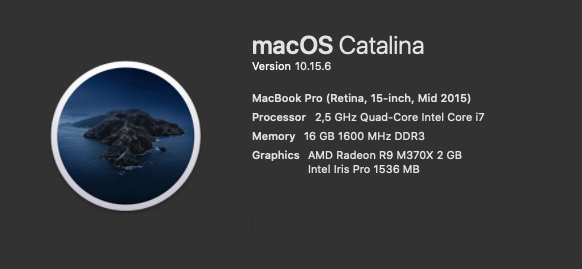
\includegraphics[scale=0.5]{cap5_experimentacion/images/computer_specs.png}
    \caption{Especificaciones del ordenador empleado en la experimentación.}
    \label{fig:computer_specs}
\end{figure}

\subsection{Métricas empleadas y elementos analizados}

El usuario puede guardar resultados obtenidos de los experimentos en estructuras llamadas \textbf{\textit{dataframe}}. \\

Un dataframe es un tipo de estructura que se caracteriza por guardar los datos y organizarlos por columnas y por filas. Cada fila de dicha estructura se corresponde con una iteración del experimento. Los resultados contienen los siguientes campos: 
\begin{enumerate}
    \item \texttt{experimentType}: El tipo de experimento realizado. 
    \item \texttt{modelUsed}: El modelo del agente empleado.
    \item \texttt{episodes}: El total de episodios por iteración.
    \item \texttt{iterations}: El total de iteraciones realizadas. 
    \item \texttt{episode\_results}: Lista de objetos que contiene los resultados de interés de los episodios de cada iteración, en concreto:
    \begin{itemize}
        \item \texttt{episodes}: Número total de episodios por iteración, que se emplea aquí para calcular el error obtenido.
        \item \texttt{steps\_to\_completion}: Lista que contiene el total de pasos realizados en cada episodio para buscar el objetivo. El total de pasos que se pueden realizar pueden estar entre el número óptimo de acciones, que se corresponde a la distancia Manhattan entre el agente y el objetivo, y el número máximo de pasos permitidos para alcanzar el objetivo. Si el número de pasos alcanza el máximo, generalmente significa que no se ha encontrado una solución. 
        \item \texttt{total\_solved}: Número total de episodios en los que se ha encontrado una solución.
        \item \texttt{episode\_reward}: Lista de recompensas para cada episodio.
        \item \texttt{error}: Porcentaje de episodios que han llegado a una solución.
        \item \texttt{distance\_to\_goal}: Distancia entre el agente y el objetivo. 
        \item \texttt{action\_combinations}: Lista que contiene la secuencia de acciones realizadas por episodio para alcanzar el objetivo. Dado que las secuencias se repiten, solamente se guardan aquellas secuencias que han aparecido más de 5 veces en la ejecución. 
    \end{itemize}
    \item \texttt{dimension}: Las dimensiones del entorno. 
    \item \texttt{start\_pos}: La posición inicial del agente.
    \item \texttt{goal\_pos}: La posición del objetivo. 
\end{enumerate}

Las gráficas realizadas con los resultados obtenidos muestra la evolución del total de acciones, de las recompensas recibidas y de la variación de las acciones a lo largo de los episodios realizados. Además, también se muestran las secuencias de acciones más frecuentes que ha aprendido el agente para alcanzar el objetivo, y el número total de veces que dichas secuencias se han aplicado. 

\subsection{Arquitectura de la red neuronal del agente}

A lo largo de la experimentación se ha mantenido estable la arquitectura de la red neuronal del agente. Tal como se ha explicado en el apartado de diseño del agente \ref{diseñoAgente}, la red neuronal consta de 4 capas de 4, 25, 25 y 4 neuronas respectivamente. La red se muestra en la Fig.~\ref{fig:NN4_25_25_4}. \\

No se ha modificado la red en cada experimento porque se ha considerado que si se modifica, la comparación de los resultados no sería válida debido a que no puede determinar qué resultados son mejores si los experimentos no se han llevado a cabo bajo las mismas circunstancias. 

\section{Tipos de experimentos} \label{tiposExperimentos}

Para este trabajo se han implementado 4 tipos de experimentos que puede invocar el usuario:

\begin{enumerate}
    \item \textbf{Estudio de convergencia:} Entorno estático.  Se trata de un experimento estático que \textit{mantiene la misma distancia entre el agente y el objetivo} a lo largo de su ejecución. El objetivo de este experimento es observar si llega un punto en el que el resultado converge en una solución. 
    \item \textbf{Alternando el inicio del agente:} Entorno dinámico. Se realiza el experimento \textit{modificando la posición inicial del agente} con cada iteración de la ejecución. El objetivo de este experimento es observar la adaptación del agente frente al cambio de distancia entre su posición inicial y la del objetivo, y si incluso con un entorno estático consigue encontrar la solución.
    \item \textbf{Alternando la posición del objetivo:} Entorno dinámico. Se realiza el experimento \textit{modificando la posición del objetivo} con cada iteración de la ejecución. El objetivo de este experimento es el mismo que el anterior.
    \item \textbf{Repetir experimento} ya realizando modificando sus condiciones. Entorno dinámico. Este tipo de experimento sólo se puede efectuar con los experimentos de alternación de las posiciones del agente y del objetivo. Dichos experimentos necesariamente deben realizar varias iteraciones ya que se trata de modificar las distancias y ver el comportamiento de la red. Cada iteración, por lo tanto, tiene una distancia concreta. El objetivo de este experimento es ir alternando las distancias de cada iteración y observar si se obtienen resultados distintos al experimento original. 
\end{enumerate}

 
\section{Experimentos realizados}

En todos los episodios, en caso de que no se especifique, se ha empleado un \textit{learning rate} de 0.01, un \textit{exploration rate} de 0.2 y un máximo de pasos que se pueden realizar para alcanzar el objetivo de 60. Se han elegido estos valores tras la realización de varias pruebas iniciales. \\

En la Fig.~\ref{fig:initial} se pueden observar los resultados de un experimento de 1 iteración de 100 episodios y empleando los valores especificados anteriormente. La distancia al objetivo es de 4. Las acciones realizadas (Fig.~\ref{fig:initial_acciones}) se estabilizan en el valor óptimo 4 y no varía mucho su distribución (Fig.~\ref{fig:initial_boxplot}); además, las recompensas con máximas a lo largo de la ejecución (Fig.~\ref{fig:initial_recompensa}) y de los 100 episodios se han resuelto 97 (Fig.~\ref{fig:initial_porcentajeResuelto}). Los resultados obtenidos son muy buenos, por lo que se utilizarán dichos valores en todos los experimentos. \\

\begin{figure}
    \centering
    \begin{subfigure}{.6\textwidth}
        \centering
        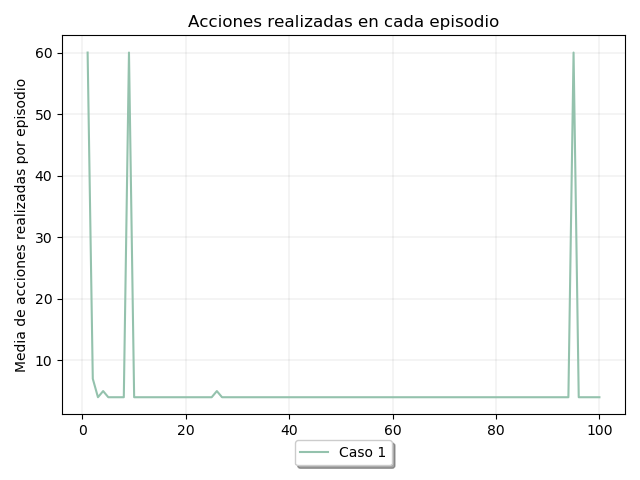
\includegraphics[scale=0.35]{cap5_experimentacion/images/initial_acciones.png}
        \caption{Aplicada 313 veces.}
        \label{fig:initial_acciones}
    \end{subfigure}%      
    \begin{subfigure}{.6\textwidth}
        \centering
        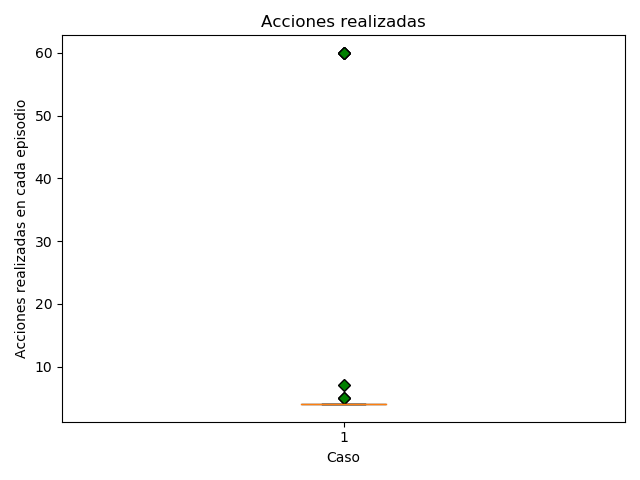
\includegraphics[scale=0.35]{cap5_experimentacion/images/initial_boxplot.png}
        \caption{Aplicada 86 veces.}
        \label{fig:initial_boxplot}
    \end{subfigure}
    \begin{subfigure}{.6\textwidth}
        \centering
        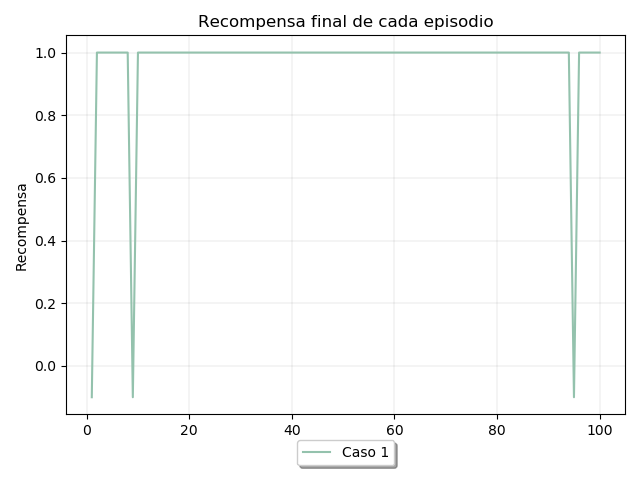
\includegraphics[scale=0.35]{cap5_experimentacion/images/initial_recompensa.png}
        \caption{Aplicada 29 veces.}
        \label{fig:initial_recompensa}
    \end{subfigure}%
    \begin{subfigure}{.6\textwidth}
        \centering
        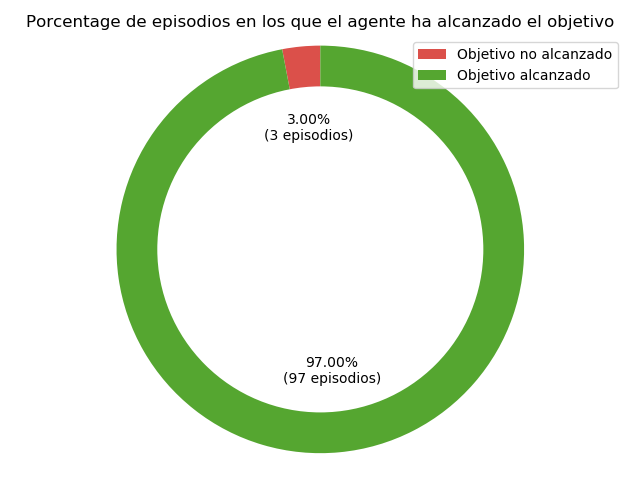
\includegraphics[scale=0.35]{cap5_experimentacion/images/initial_porcentajeResuelto.png}
        \caption{Aplicada 29 veces.}
        \label{fig:initial_porcentajeResuelto}
    \end{subfigure}
    \caption{Experimento de prueba de una iteración de 100 episodios, con \textit{learning rate} de 0.01, \textit{exploration rate} 0.2 y 60 pasos máximos permitidos.}
    \label{fig:initial}
\end{figure}

A continuación se explican los 5 experimentos realizados para determinar la capacidad de la red interna del agente de encontrar una solución para el problema dado. Los distintos experimentos que se han realizado son: 

\begin{enumerate}
    \item \texttt{EPS1}: Estudio de convergencia en un entorno 5x5.
    \item \texttt{EPS2}: Estudio de convergencia con \textit{learning rate} variable.
    \item \texttt{EPS3}: Estudio de convergencia con \textit{exploration rate} variable.
    \item \texttt{CHG\_ORG}: Alternando el inicio del agente en un entorno 5x5.
    \item \texttt{CHG\_GOAL}: Alternando la posición del objetivo en un entorno 5x5.
\end{enumerate}

En todos los experimentos realizados se considera que el \textbf{valor óptimo de acciones} que se pueden realizar para alcanzar el objetivo es equivalente a la distancia Manhattan que hay entre la posición inicial del agente y la posición del objetivo.  

\subsection{EPS1: Estudio de convergencia en un entorno 5x5} \label{EPS1}

Este experimento se ha realizado con 1 iteración de 500 episodios. La posición inicial del agente se ha definido en (0, 0) y la posición del objetivo en (4, 4). La distancia entre el agente y su objetivo es de 8 y se corresponde, además, a la distancia máxima que existe dentro del entorno actual. En la Fig.~\ref{fig:dim5_EPS1} se puede visualizar el entorno del problema con su configuración. \\

\begin{figure}
    \centering
    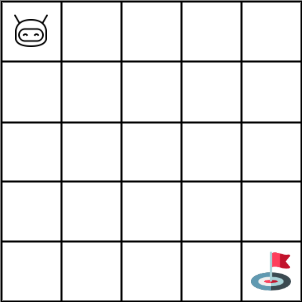
\includegraphics[scale=0.4]{cap5_experimentacion/images/dim5.png}
    \caption{Configuración del entorno para el experimento \texttt{EPS1}.}
    \label{fig:dim5_EPS1}
\end{figure}

El número óptimo de acciones que se pueden hacer para alcanzar el objetivo es 8. 

\subsubsection{Análisis de las acciones realizadas} 

Se puede observar en la Fig.~\ref{fig:dim5_acciones} que a partir de los 80 episodios aproximadamente el número de acciones se estabiliza, alcanzando además el número óptimo de pasos que se deben realizar. Aunque a lo largo de los episodios el número de acciones realizadas alcanza varias veces el valor máximo, no significa que el agente no esté aprendiendo bien. De hecho, es una muestra de que sigue aprendiendo y explorando nuevas secuencias de acciones para realizar.\\

\begin{figure}
    \centering
    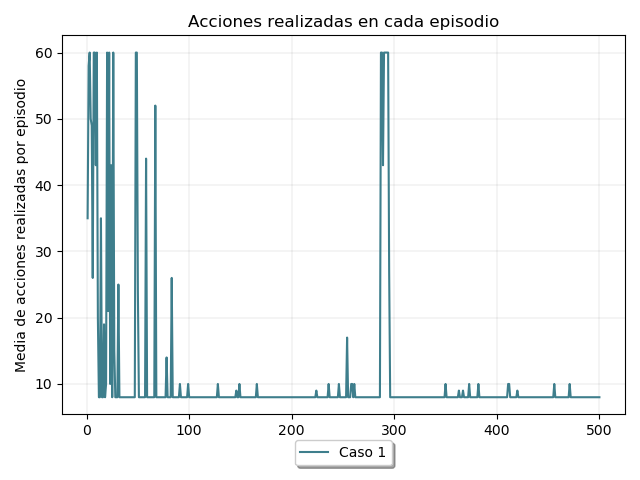
\includegraphics[scale=0.4]{cap5_experimentacion/images/dim5_acciones.png}
    \caption{Acciones realizadas por episodio en el experimento \texttt{EPS1}.}
    \label{fig:dim5_acciones}
\end{figure}

En la Fig.~\ref{fig:dim5_boxplot} se muestra la distribución de las acciones totales realizadas en el experimento. La media de las acciones se corresponde con el valor óptimo, en este caso 8. También se pueden observar otro tipo de elementos en este gráfico: los valores atípicos. Un valor se considera atípico siempre sea una observación que es numéricamente distante del resto de los datos. \\
 
\begin{figure}
    \centering
    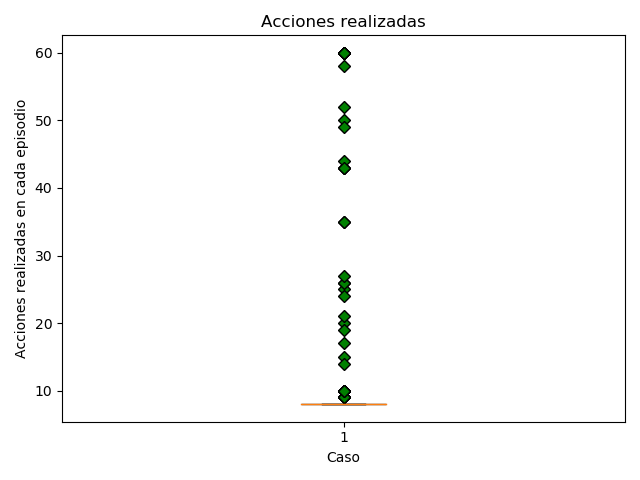
\includegraphics[scale=0.4]{cap5_experimentacion/images/dim5_boxplot.png}
    \caption{Boxplot del experimento \texttt{EPS1}.}
    \label{fig:dim5_boxplot}
\end{figure}

Otro análisis realizado es el estudio de las secuencias de acciones que el modelo ha aprendido para alcanzar el objetivo. Cabe destacar que las secuencias mostradas son las más \textit{frecuentes}. Se considera que una secuencia es frecuente si aparece como solución en más de 5 episodios. Por lo tanto, la suma de las veces que se han aplicado las secuencias frecuentes \textbf{no} es necesariamente equivalente al total de episodios resueltos del experimento. \\

Como bien se observa en la 
Fig.~\ref{fig:dim5_actions}, se han encontrado 4 secuencias diferentes de 8 acciones que llevan al objetivo. La secuencia más frecuente ha sido la de la Fig.~\ref{fig:dim5_actions_313}, con un total de 313 veces que ha sido aplicada. El total de episodios resueltos empleando estas secuencias es de 433.
 
\begin{figure}
    \centering
    \begin{subfigure}{.5\textwidth}
        \centering
        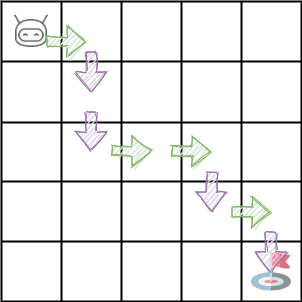
\includegraphics[scale=0.4]{cap5_experimentacion/images/dim5_actions_313.png}
        \caption{Aplicada 313 veces.}
        \label{fig:dim5_actions_313}
    \end{subfigure}%       
    \begin{subfigure}{.5\textwidth}
        \centering
        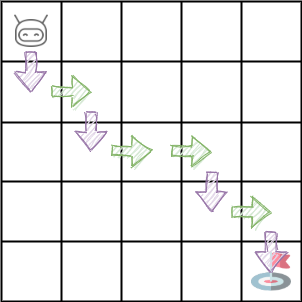
\includegraphics[scale=0.4]{cap5_experimentacion/images/dim5_actions_86.png}
        \caption{Aplicada 86 veces.}
        \label{fig:dim5_actions_86}
    \end{subfigure}
    \begin{subfigure}{.5\textwidth}
        \centering
        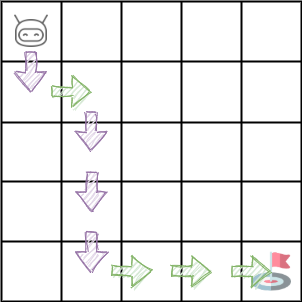
\includegraphics[scale=0.4]{cap5_experimentacion/images/dim5_actions_29.png}
        \caption{Aplicada 29 veces.}
        \label{fig:dim5_actions_29}
    \end{subfigure}%
    \begin{subfigure}{.5\textwidth}
        \centering
        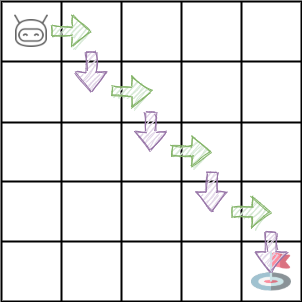
\includegraphics[scale=0.4]{cap5_experimentacion/images/dim5_actions_5.png}
        \caption{Aplicada 5 veces.}
        \label{fig:dim5_actions_5}
    \end{subfigure}
    \caption{Secuencias de acciones realizadas en el experimento \texttt{EPS1} para llegar al objetivo.}
    \label{fig:dim5_actions}
\end{figure}

\subsubsection{Análisis de las recompensas obtenidas y total de episodios resueltos} 

En cuanto a la recompensa obtenida en este experimento, se observa en la Fig.~\ref{fig:dim5_recompensa} que al inicio de la ejecución el agente obtenía valores cercanos al cero, lo que significa que recibía penalizaciones; a partir del mismo episodio en el que el agente comienza a estabilizar las acciones tomada, también se estabiliza la recompensa en su valor máximo y se mantiene en ésta. Recordemos que la recompensa máxima que tiene como valor 1 significa que el agente ha alcanzado su objetivo.\\
 
\begin{figure}
    \centering
    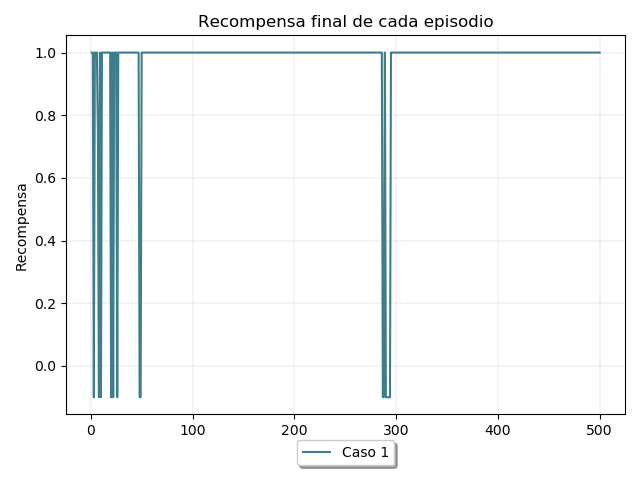
\includegraphics[scale=0.4]{cap5_experimentacion/images/dim5_recompensa.png}
    \caption{Recompensas finales de cada episodio del experimento \texttt{EPS1}.}
    \label{fig:dim5_recompensa}
\end{figure}

En este experimento de 500 episodios, el agente ha sido capaz de alcanzar el objetivo en 484 episodios. En la Fig.~\ref{fig:dim5_porcentajeResuelto} se muestran los porcentajes de episodios resueltos y no resueltos del experimento. Tal como se ha mencionado anteriormente, el total de episodios resueltos no es igual al total de episodios que se han solucionado aplicando las secuencias de la Fig.~\ref{fig:dim5_actions}. En concreto, hay 16  episodios que se han resuelto mediante unas secuencias de acciones poco frecuentes. \\

\begin{figure}
    \centering
    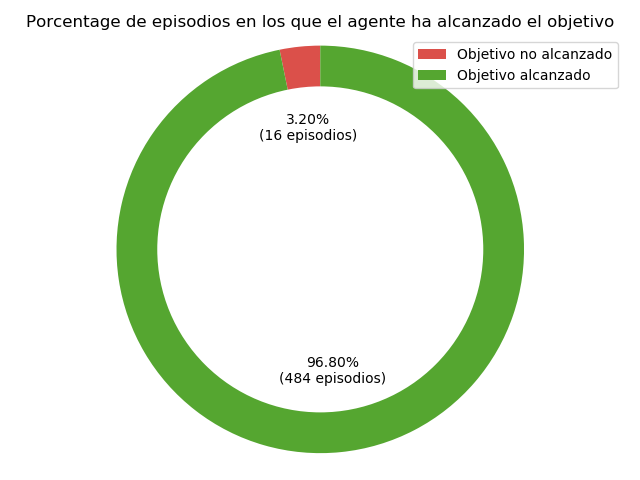
\includegraphics[scale=0.4]{cap5_experimentacion/images/dim5_porcentajeResuelto.png}
    \caption{Porcentaje de episodios en los que el agente alcanza el objetivo en el experimento \texttt{EPS1}.}
    \label{fig:dim5_porcentajeResuelto}
\end{figure}

Este estudio ha permitido ver que el agente converge hacia una secuencia de pasos óptima con un número suficiente de episodios. En los siguientes experimentos cambiaremos algunas características de la red interna del agente para analizar la nueva evolución de la convergencia con respecto a este experimento.

%TODO ISAAC HERE

\subsection{EPS2: Estudio de convergencia con learning rate variable} \label{EPS2}

Como bien se plantea en \cite{learningRate}, el \textit{learning rate} sirve para afinar el tamaño de los pasos que se realizan en los algoritmos de optimización que buscan el mínimo de la función de pérdida en el entrenamiento de la red. Determina, en cierta manera, la velocidad en la que el agente aprende. \\

El objetivo del experimento es observar cómo afecta este parámetro en el aprendizaje del agente. Como se puede observar en la Fig.~\ref{fig:learningRate}, si el paso es muy pequeño se necesita mucho tiempo para encontrar el mínimo de la función de pérdida; en cambio, si es muy grande, es muy complicado que converja y además se presentarán valores muy poco estables. \\

\begin{figure}
    \centering
    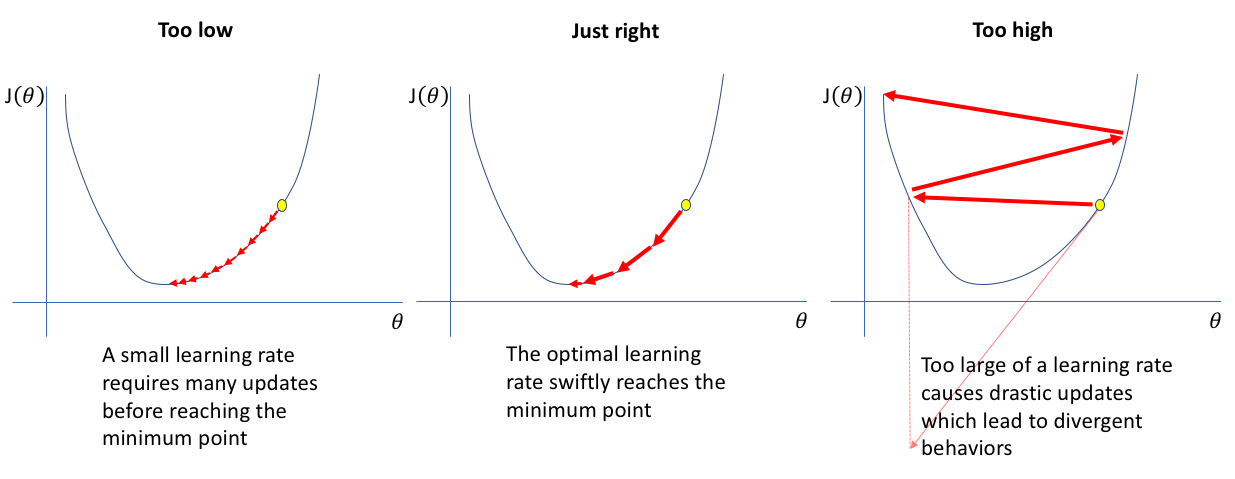
\includegraphics[scale=0.3]{cap5_experimentacion/images/learningRate.png}
    \caption{Tamaño del paso y evolución de la búsqueda según el valor del \textit{learning rate} Fuente:~\cite{learningRateImage}.}
    \label{fig:learningRate}
\end{figure}

Los experimentos explicados a continuación son de 1 iteración de 500 episodios y tienen la misma configuración que el experimento anterior (\nameref{EPS1}). La configuración se muestra en la  Fig.~\ref{fig:dim5_EPS1}. \\

El número óptimo de acciones que se pueden hacer para alcanzar el objetivo sigue siendo 8.

\subsubsection{EPS2\_LR1: Learning rate 0.001} \label{EPS2_LR1}

En este experimento se ha empleado un learning rate con valor de \textbf{0.001}. 

\paragraph{Análisis de las acciones realizadas} 

Como se puede observar en la Fig.~\ref{fig:dim5_lr0.001_ep0.2_acciones}, el número de acciones durante todo el experimento se ha mantenido estable en el valor máximo de acciones permitidas, en concreto 60. Esto implica que no se ha llegado a ninguna solución ya que no ha podido encontrar la función adecuada de aprendizaje. Lo mismo se puede apreciar en el boxplot de la Fig.~\ref{fig:dim5_lr0.001_ep0.2_boxplot}, donde se muestra que la distribución de las acciones se concentra en el valor 60. \\

\begin{figure}
    \centering
    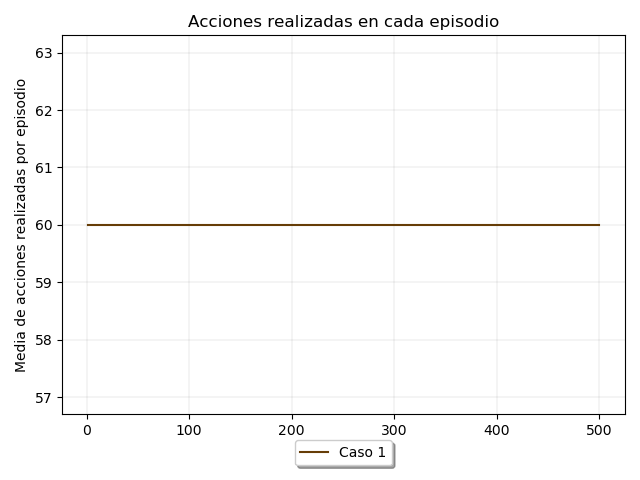
\includegraphics[scale=0.4]{cap5_experimentacion/images/dim5_lr0.001_ep0.2_acciones.png}
    \caption{Acciones realizadas por episodio en el experimento \texttt{EPS2\_LR1}}
    \label{fig:dim5_lr0.001_ep0.2_acciones}
\end{figure}

\begin{figure}
    \centering
    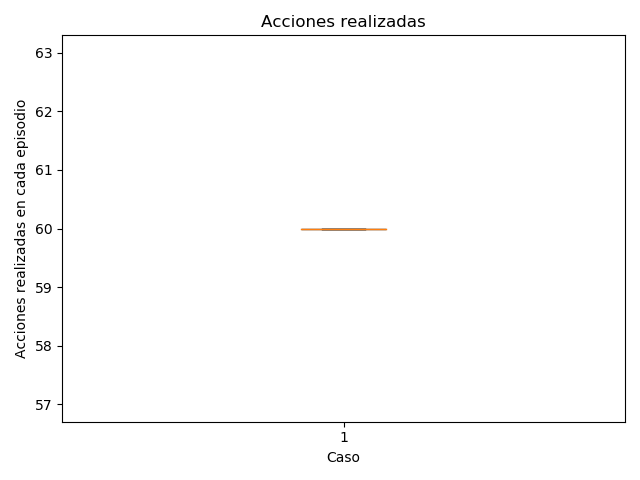
\includegraphics[scale=0.4]{cap5_experimentacion/images/dim5_lr0.001_ep0.2_boxplot.png}
    \caption{Boxplot del experimento \texttt{EPS2\_LR1}.}
    \label{fig:dim5_lr0.001_ep0.2_boxplot}
\end{figure}

Además, como bien era de esperar, no se ha podido encontrar ninguna secuencia de pasos para alcanzar el objetivo. Queda demostrado que para este problema y con estas características concretas, un  \textit{learning rate} bajo no aporta buenos resultados; para que los resultados mejoren, posiblemente sea necesario incrementar el número de pasos que el agente puede realizar para alcanzar el objetivo, ya que supondría que el algoritmo tiene más iteraciones en las que se puede buscar el valor mínimo de la función de pérdida. 

\paragraph{Análisis de las recompensas obtenidas y total de episodios resueltos} 

En cuanto a las recompensas, se muestran en la Fig.~\ref{fig:dim5_lr0.001_ep0.2_recompensa}. Se puede apreciar que a lo largo de la ejecución el agente ha recibido un elevado número de penalizaciones y durante un gran nombre de episodios consecutivos. Sin embargo, se puede observar que en distintas ocasiones el agente ha ido incrementando su recompensa, llegando a valores superiores a 0.6. Es posible que en el caso de que hubiese tenido un número mayor de pasos permitidos por episodio, el agente haya alcanzado su objetivo en algún episodio. \\

\begin{figure}
    \centering
    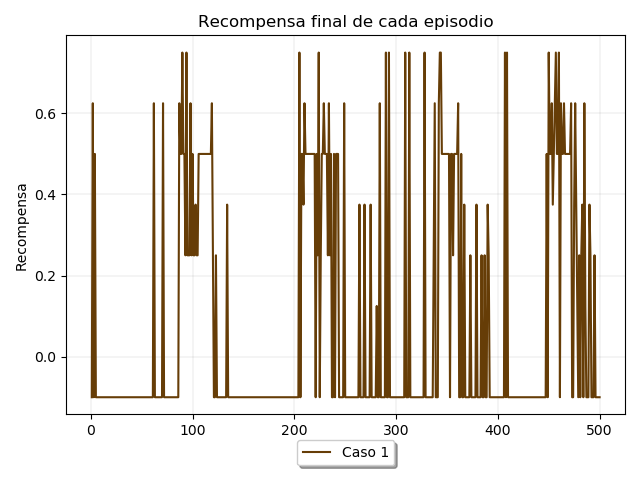
\includegraphics[scale=0.4]{cap5_experimentacion/images/dim5_lr0.001_ep0.2_recompensa.png}
    \caption{Recompensas finales de cada episodio del experimento \texttt{EPS2\_LR1}.}
    \label{fig:dim5_lr0.001_ep0.2_recompensa}
\end{figure}

Como se puede observar en la Fig.~\ref{fig:dim5_lr0.001_ep0.2_porcentajeResuelto}, en este experimento de 500 episodios el agente no ha sido capaz de alcanzar el objetivo.

\begin{figure}
    \centering
    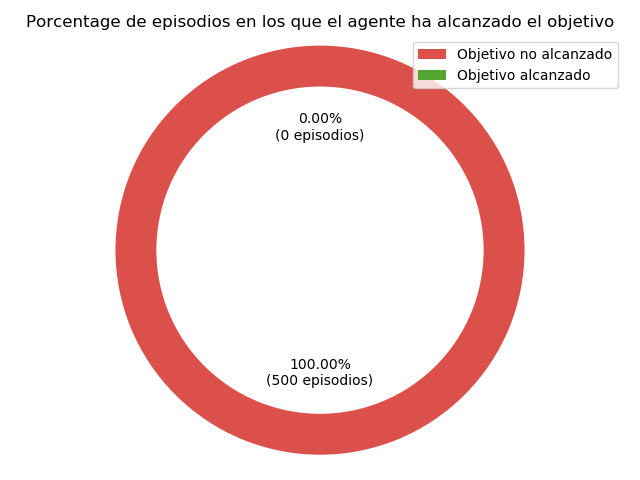
\includegraphics[scale=0.4]{cap5_experimentacion/images/dim5_lr0.001_ep0.2_porcentajeResuelto.png}
    \caption{Porcentaje de episodios en los que el agente alcanza el objetivo en el experimento \texttt{EPS2\_LR1}.}
    \label{fig:dim5_lr0.001_ep0.2_porcentajeResuelto}
\end{figure}

\subsubsection{EPS2\_LR2: Learning rate 0.01} \label{EPS2_LR2}

En este experimento se ha empleado un learning rate con valor de \textbf{0.01}. 

\paragraph{Análisis de las acciones realizadas}

Como bien se puede observar en la Fig.~\ref{fig:dim5_lr0.01_ep0.2_acciones}, la diferencia de resultados obtenidos respecto al experimento anterior (\nameref{EPS2_LR1}) es evidente: el total de acciones realizadas se mantiene en el valor óptimo a lo largo del experimento, con pocos episodios en los que este valor es mayor. \\

\begin{figure}
    \centering
    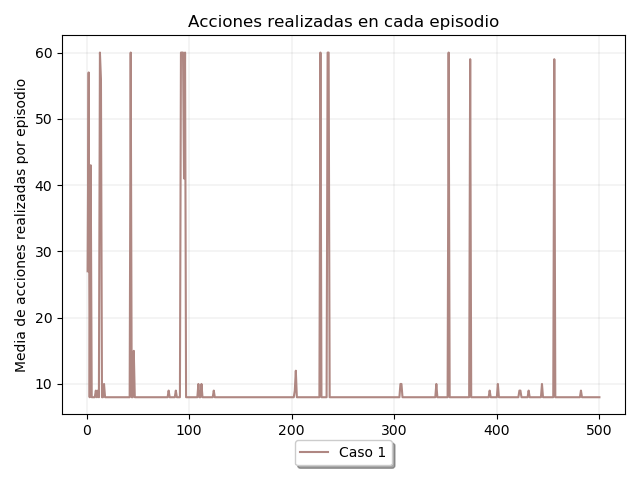
\includegraphics[scale=0.4]{cap5_experimentacion/images/dim5_lr0.01_ep0.2_acciones.png}
        \caption{Acciones realizadas por episodio en el experimento \texttt{EPS2\_LR2}.}
    \label{fig:dim5_lr0.01_ep0.2_acciones}
\end{figure}

Asimismo, el boxplot de la figura Fig.~\ref{fig:dim5_lr0.01_ep0.2_boxplot} muestra que la media de acciones está en el valor óptimo. \\

\begin{figure}
    \centering
    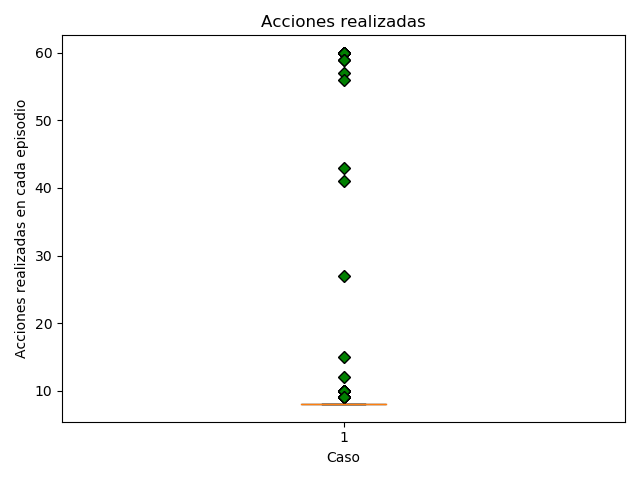
\includegraphics[scale=0.4]{cap5_experimentacion/images/dim5_lr0.01_ep0.2_boxplot.png}
    \caption{Boxplot del experimento \texttt{EPS2\_LR2}.}
    \label{fig:dim5_lr0.01_ep0.2_boxplot}
\end{figure}

En cuanto a las secuencias de acciones realizadas, hay una única acción predominante y se muestra en la Fig.~\ref{fig:dim5_lr0.01_ep0.2_458}. Dicha secuencia se ha aplicado en 458 episodios del total de 500.  \\

\begin{figure}
    \centering
    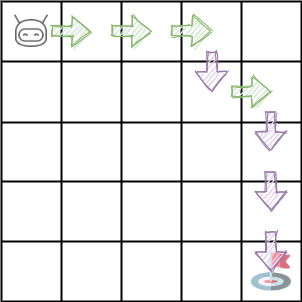
\includegraphics[scale=0.4]{cap5_experimentacion/images/dim5_lr0.01_ep0.2_458.png}
    \caption{Secuencia de acciones realizada en el experimento \texttt{EPS2\_LR2} para llegar al objetivo. Aplicada 458 veces.}
    \label{fig:dim5_lr0.01_ep0.2_458}
\end{figure}

\paragraph{Análisis de las recompensas obtenidas y total de episodios resueltos} 

En cuanto a las recompensas, se muestran en la Fig.~\ref{fig:dim5_lr0.01_ep0.2_recompensa}. Se puede apreciar que a lo largo de la ejecución la recompensa que obtiene el agente se mantiene estable en el valor máximo, con pocos episodios en los que ha recibido penalizaciones.  \\

\begin{figure}
    \centering
    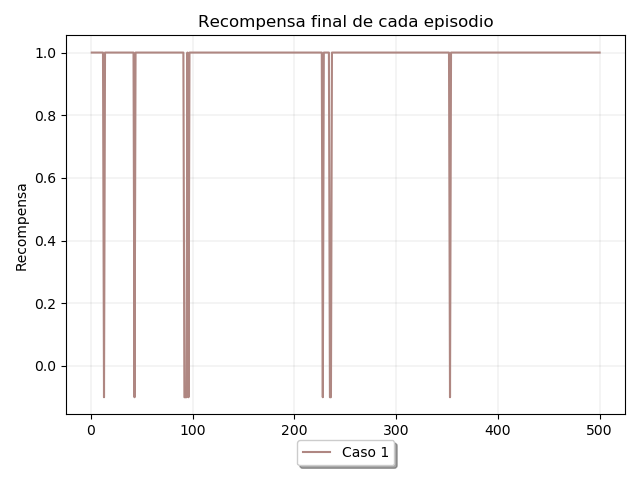
\includegraphics[scale=0.43]{cap5_experimentacion/images/dim5_lr0.01_ep0.2_recompensa.png}
    \caption{Recompensas finales de cada episodio del experimento \texttt{EPS2\_LR2}.}
    \label{fig:dim5_lr0.01_ep0.2_recompensa}
\end{figure}

En este experimento de 500 episodios el agente ha sido capaz de alcanzar el objetivo en 490 episodios. En la Fig.~\ref{fig:dim5_lr0.01_ep0.2_porcentajeResuelto} se observan los porcentajes de episodios resueltos. \\

\begin{figure}
    \centering
    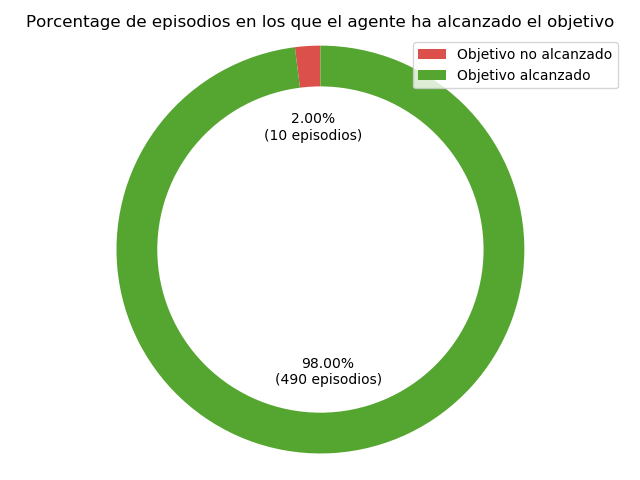
\includegraphics[scale=0.4]{cap5_experimentacion/images/dim5_lr0.01_ep0.2_porcentajeResuelto.png}
    \caption{Porcentaje de episodios en los que el agente alcanza el objetivo en el experimento \texttt{EPS2\_LR2}.}
    \label{fig:dim5_lr0.01_ep0.2_porcentajeResuelto}
\end{figure}

\subsubsection{EPS2\_LR3: Learning rate 0.1} \label{EPS2_LR3}

En este experimento se ha empleado el learning rate con valor de \textbf{0.1}. \\

\paragraph{Análisis de las acciones realizadas}

De la misma manera que ha ocurrido en el experimento \nameref{EPS2_LR1}, las acciones totales realizadas se mantienen estables en el valor máximo permitido, tal como se puede observar en la Fig.~\ref{fig:dim5_lr0.001_ep0.2_acciones} y el boxplot de la Fig.~\ref{fig:dim5_lr0.001_ep0.2_boxplot}. \\

\begin{figure}
    \centering
    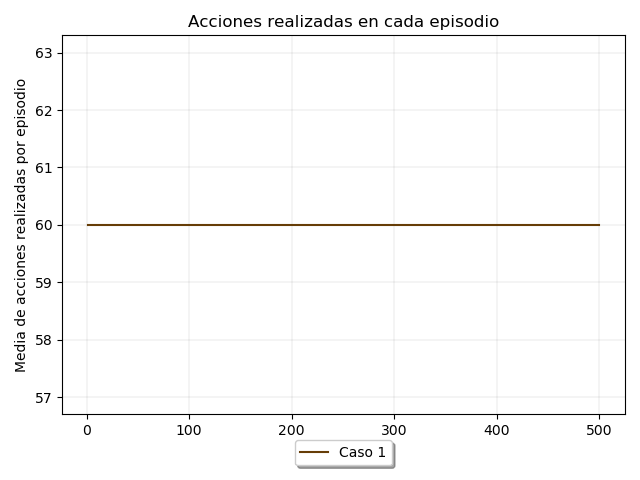
\includegraphics[scale=0.4]{cap5_experimentacion/images/dim5_lr0.001_ep0.2_acciones.png}
   \caption{Acciones realizadas por episodio en el experimento \texttt{EPS2\_LR3}.}
    \label{fig:dim5_lr0.1_ep0.2_acciones}
\end{figure}

\begin{figure}
    \centering
    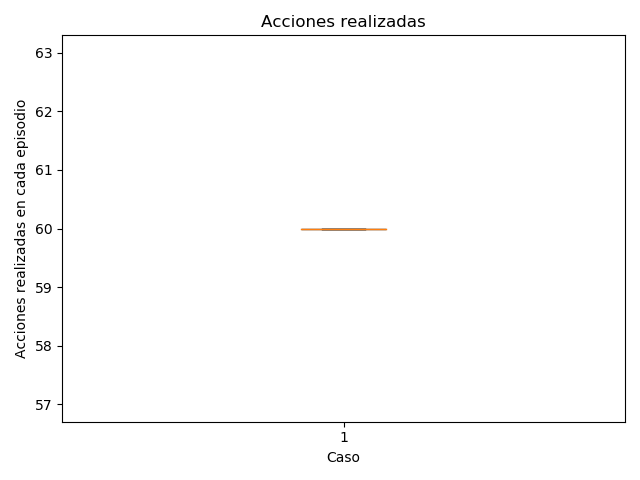
\includegraphics[scale=0.4]{cap5_experimentacion/images/dim5_lr0.001_ep0.2_boxplot.png}
    \caption{Boxplot del experimento \texttt{EPS2\_LR3}.}
    \label{fig:dim5_lr0.1_ep0.2_boxplot}
\end{figure}

En este experimento no ha sido posible detectar ninguna secuencia de acciones que permita al agente alcanzar el objetivo. 

\paragraph{Análisis de las recompensas obtenidas y total de episodios resueltos} 

Por otro lado, respecto a las recompensas obtenidas en el experimento \nameref{EPS2_LR1}, las recompensas de este experimento han sido inferiores. El agente ha recibido constantemente penalizaciones, y en número escaso de episodios ha recibido una recompensa que no superaba el 0.65, aproximadamente.\\

\begin{figure}
    \centering
    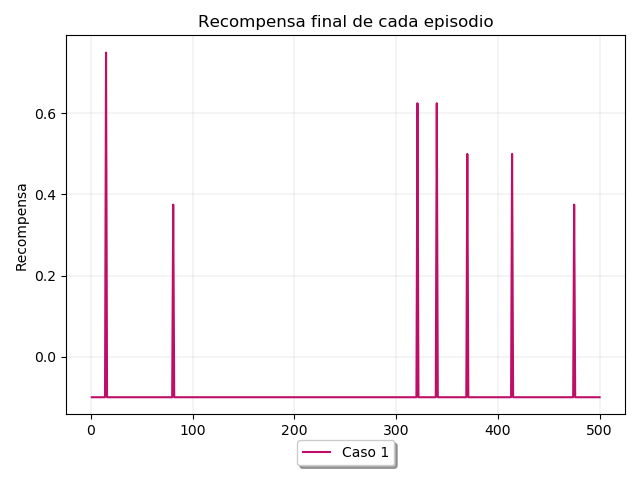
\includegraphics[scale=0.4]{cap5_experimentacion/images/dim5_lr0.1ep0.2_recompensa.png}
    \caption{Recompensas finales de cada episodio del experimento \texttt{EPS2\_LR3}.}
    \label{fig:dim5_lr0.1_ep0.2_recompensa}
\end{figure}

En este experimento de 500 episodios el agente no ha sido capaz de alcanzar el objetivo, tal como se puede observar en la Fig.~\ref{fig:dim5_lr0.1ep0.2_porcentajeResuelto}.

\begin{figure}
    \centering
    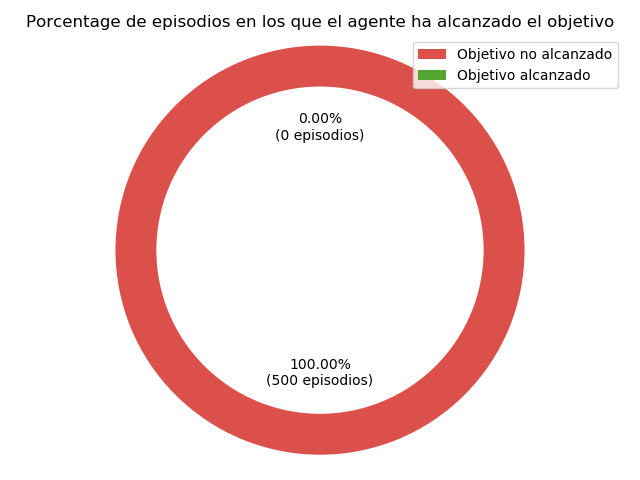
\includegraphics[scale=0.4]{cap5_experimentacion/images/dim5_lr0.1ep0.2_porcentajeResuelto.png}
    \caption{Porcentaje de episodios en los que el agente alcanza el objetivo en el experimento \texttt{EPS2\_LR3}.}
    \label{fig:dim5_lr0.1ep0.2_porcentajeResuelto}
\end{figure}

\subsection{EPS3: Estudio de convergencia  con exploration rate variable} \label{EPS3}

Recordemos que en el apartado de \textbf{\nameref{explorationExploitation}} se ha comentado el dilema de balancear adecuadamente la exploración del entorno y la explotación de los conocimientos ya adquiridos para realizar un aprendizaje eficiente. \\

Este experimento tiene como objetivo observar cómo afecta el \textit{exploration rate}, es decir, la exploración del entorno, al aprendizaje del agente. \\

Los experimentos explicados a continuación son de 1 iteración de 500 episodios y tienen la misma configuración que el experimento anterior (\nameref{EPS1}). La configuración se muestra en la  Fig.~\ref{fig:dim5_EPS1}. \\

El número óptimo de acciones que se pueden hacer para alcanzar el objetivo sigue siendo 8.\\ 


\subsubsection{EPS3\_ER1: Exploration rate 0} \label{EPS3_ER1}

En este experimento el \textit{exploration rate} es de 0, de modo que no se explora el entorno y sólo se emplean los conocimientos ya desarrollados por el agente. Puesto que el agente no ha sido entrenado previamente, intentará alcanzar el objetivo empleando los pesos iniciales de su red interna. 

\paragraph{Análisis de las acciones realizadas}

Como se puede observar en la Fig.~\ref{fig:dim5_lr0.01_ep0_acciones}, el agente ha sido capaz de encontrar el número óptimo de acciones por realizar y ha mantenido de manera relativamente estable este valor a lo largo del experimento; siguen habiendo episodios con el máximo de acciones realizadas, pero comparando con los resultados de los experimentos realizados hasta este punto, se pueden considerar buenos resultados. \\

\begin{figure}
    \centering
    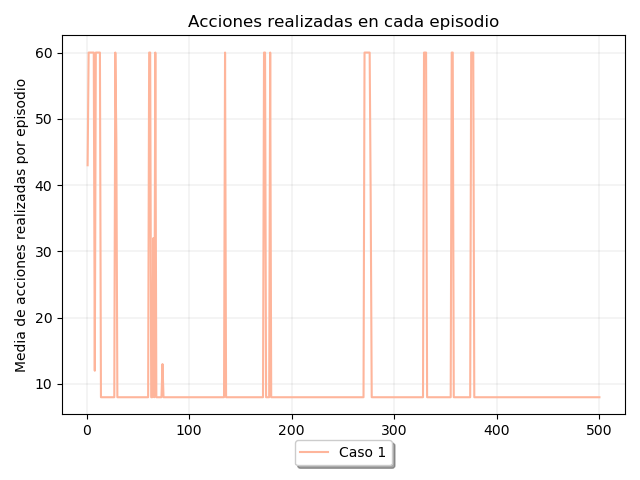
\includegraphics[scale=0.4]{cap5_experimentacion/images/dim5_lr0.01_ep0_acciones.png}
    \caption{Acciones realizadas por episodio en el experimento \texttt{EPS3\_ER1}.}
    \label{fig:dim5_lr0.01_ep0_acciones}
\end{figure}

En el boxplot de la Fig.~\ref{fig:dim5_lr0.01_ep0_boxplot} se muestra la distribución de los datos y se puede observar como la media de las acciones realizadas está en el valor óptimo (8).\\

\begin{figure}
    \centering
    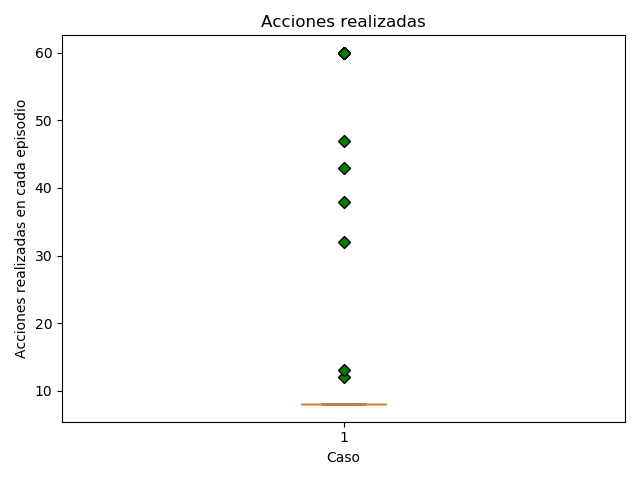
\includegraphics[scale=0.4]{cap5_experimentacion/images/dim5_lr0.01_ep0_boxplot.png}
    \caption{Boxplot del experimento \texttt{EPS3\_ER1}.}
    \label{fig:dim5_lr0.01_ep0_boxplot}
\end{figure}

En la Fig.~\ref{fig:dim5_lr0.01_ep0_453} se puede observar la secuencia de acciones empleada en este experimento para alcanzar el objetivo. De 500 episodios se ha aplicado 453 veces para alcanzar la solución. 

\begin{figure}
    \centering
    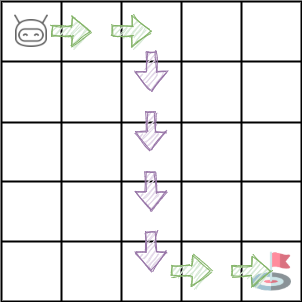
\includegraphics[scale=0.4]{cap5_experimentacion/images/dim5_lr0.01_ep0_453.png}
    \caption{Secuencia de acciones del experimento \texttt{EPS3\_ER1}. Aplicada 453 veces.}
    \label{fig:dim5_lr0.01_ep0_453}
\end{figure}

\paragraph{Análisis de las recompensas obtenidas y total de episodios resueltos} 

En cuanto a las recompensas recibidas en este experimento, se aprecia en la Fig.~\ref{fig:dim5_lr0.01_ep0_recompensa} que se ha mantenido estable alrededor del valor máximo y, además, no ha recibido un número elevado de penalizaciones.  \\

\begin{figure}
    \centering
    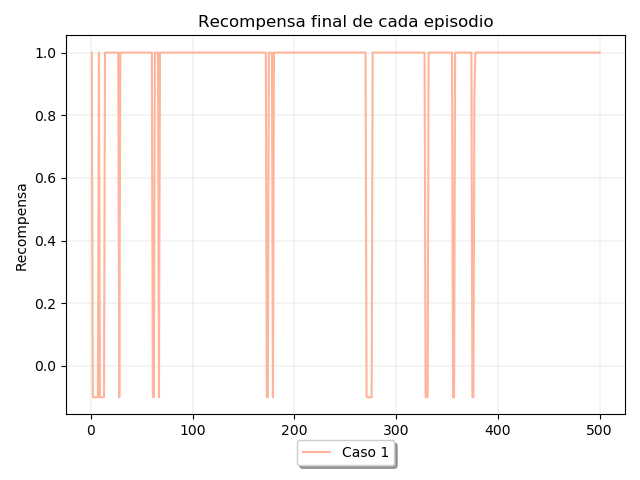
\includegraphics[scale=0.4]{cap5_experimentacion/images/dim5_lr0.01_ep0_recompensa.png}
    \caption{Recompensas finales de cada episodio del experimento \texttt{EPS3\_ER1}.}
    \label{fig:dim5_lr0.01_ep0_recompensa}
\end{figure}

En este experimento de 500 episodios el agente ha sido capaz de alcanzar el objetivo en 468 episodios. En la Fig.~\ref{fig:dim5_lr0.01_ep0_porcentajeResuelto} se muestran los porcentajes de episodios resueltos y no resueltos del experimento. 
\begin{figure}
    \centering
    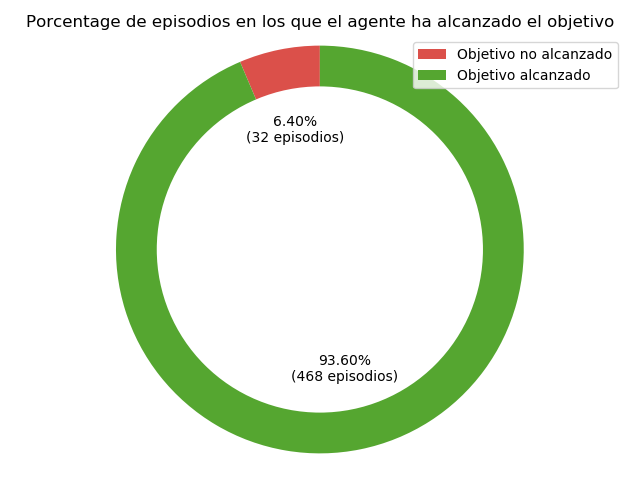
\includegraphics[scale=0.4]{cap5_experimentacion/images/dim5_lr0.01_ep0_porcentajeResuelto.png}
    \caption{Porcentaje de episodios en los que el agente alcanza el objetivo en el experimento \texttt{EPS3\_ER1}.}
    \label{fig:dim5_lr0.01_ep0_porcentajeResuelto}
\end{figure}

\subsubsection{EPS3\_ER2: Exploration rate 0.1} \label{EPS3_ER2}

En este experimento el \textit{exploration rate} es de 0.1, de modo que se explora el entorno el 10\% de las veces y el 90\% restante se emplean los conocimientos ya adquiridos. \\

\paragraph{Análisis de las acciones realizadas}

A diferencia del experimento anterior \nameref{EPS3_ER1}, el agente no consigue alcanzar en ningún momento el valor óptimo de acciones, sino que a lo largo del experimento ha realizado el número máximo de acciones permitido. Dichas recompensas se muestran en la Fig.~\ref{fig:dim5_lr0-01_ep0.1_acciones}. \\

\begin{figure}
    \centering
    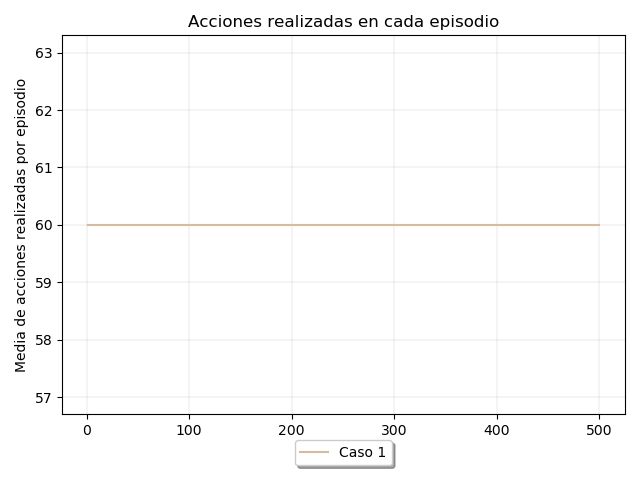
\includegraphics[scale=0.4]{cap5_experimentacion/images/dim5_lr0-01_ep0.1_acciones.png}
    \caption{Acciones realizadas por episodio en el experimento \texttt{EPS3\_ER2}.}
    \label{fig:dim5_lr0-01_ep0.1_acciones}
\end{figure}

En el boxplot de la Fig.~\ref{fig:dim5_lr0-01_ep0.1_boxplot} se aprecia que la distribución de los datos tiene la media en el valor 60.  \\
 
\begin{figure}
    \centering
    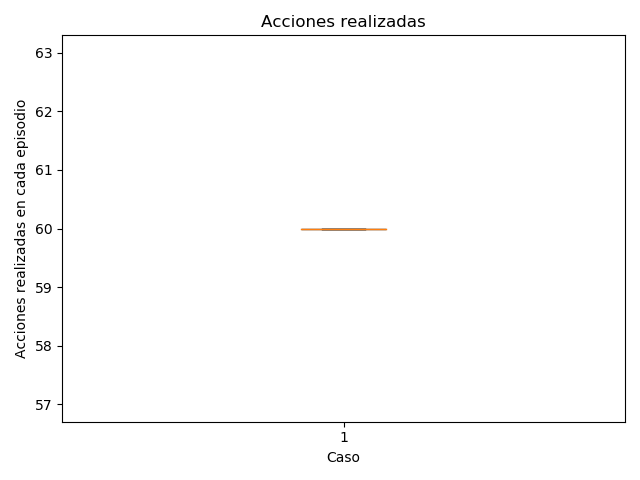
\includegraphics[scale=0.4]{cap5_experimentacion/images/dim5_lr0-01_ep0.1_boxplot.png}
    \caption{Boxplot del experimento \texttt{EPS3\_ER2}.}
    \label{fig:dim5_lr0-01_ep0.1_boxplot}
\end{figure}

No se ha conseguido encontrar ninguna secuencia de acciones que lleve al objetivo en este experimento. 

\paragraph{Análisis de las recompensas obtenidas y total de episodios resueltos} 

Tal como se observa en la Fig.~\ref{fig:dim5_lr0-01_ep0.1_recompensa}, las recompensas recibidas a lo largo del experimento son negativas, y las recompensas positivas no superan el 0.6.\\

\begin{figure}
    \centering
    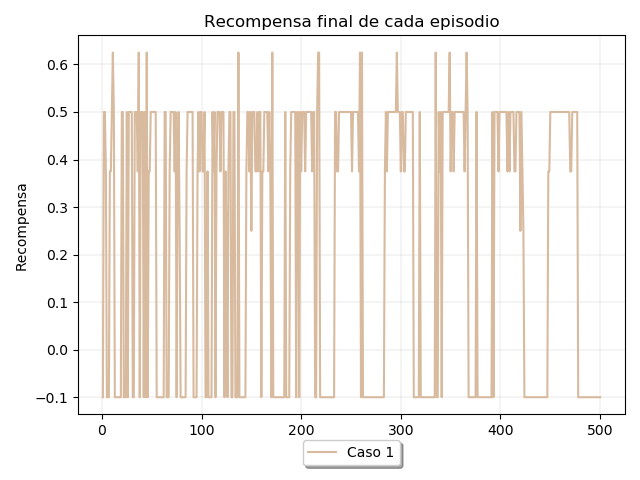
\includegraphics[scale=0.4]{cap5_experimentacion/images/dim5_lr0-01_ep0.1_recompensa.png}
    \caption{Recompensas finales de cada episodio del experimento \texttt{EPS3\_ER2}.}
    \label{fig:dim5_lr0-01_ep0.1_recompensa}
\end{figure}

En este experimento de 500 episodios el agente no ha sido capaz de alcanzar el objetivo tal como se puede observar en la Fig.~\ref{fig:dim5_lr0-01_ep0.1_porcentajeResuelto}. 

\begin{figure}
    \centering
    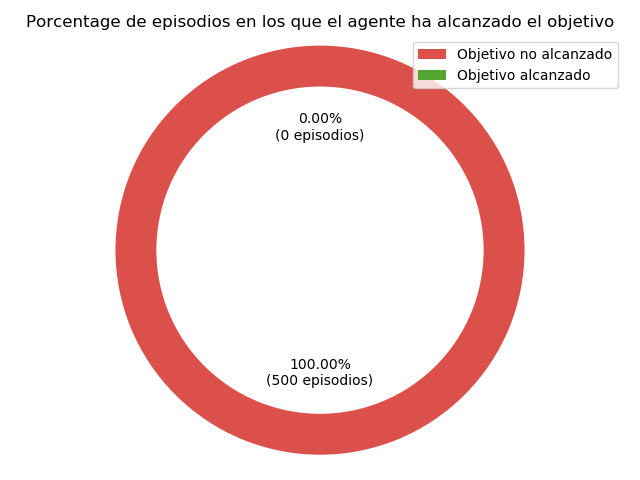
\includegraphics[scale=0.4]{cap5_experimentacion/images/dim5_lr0-01_ep0.1_porcentajeResuelto.png}
    \caption{Porcentaje de episodios en los que el agente alcanza el objetivo en el experimento \texttt{EPS3\_ER2}.}
    \label{fig:dim5_lr0-01_ep0.1_porcentajeResuelto}
\end{figure}

\subsubsection{EPS3\_ER3: Exploration rate 0.2} \label{EPS3_ER3}

En este experimento el \textit{exploration rate} es de 0.2, un valor que se toma muchas veces por defecto para realizar el aprendizaje. 

\paragraph{Análisis de las acciones realizadas}

Como se puede observar en la Fig.~\ref{fig:dim5_lr0.01_ep0.2_acciones_EPS2_ER3} las acciones realizadas a lo largo del experimento alcanzan mayoritariamente el valor óptimo, con pocos episodios en los que se tome el valor máximo de acciones. \\

\begin{figure}
    \centering
    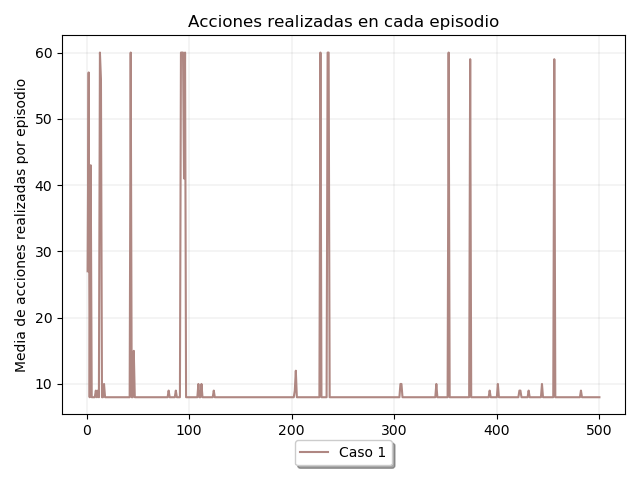
\includegraphics[scale=0.4]{cap5_experimentacion/images/dim5_lr0.01_ep0.2_acciones.png}
    \caption{Acciones realizadas por episodio en el experimento \texttt{EPS3\_ER3}.}
    \label{fig:dim5_lr0.01_ep0.2_acciones_EPS2_ER3}
\end{figure}

En boxplot de la Fig.~\ref{fig:dim5_lr0.01_ep0.2_boxplot_EPS2_ER3} se puede observar que la media de las acciones realizadas en este experimento está en el valor óptimo. 

\begin{figure}
    \centering
    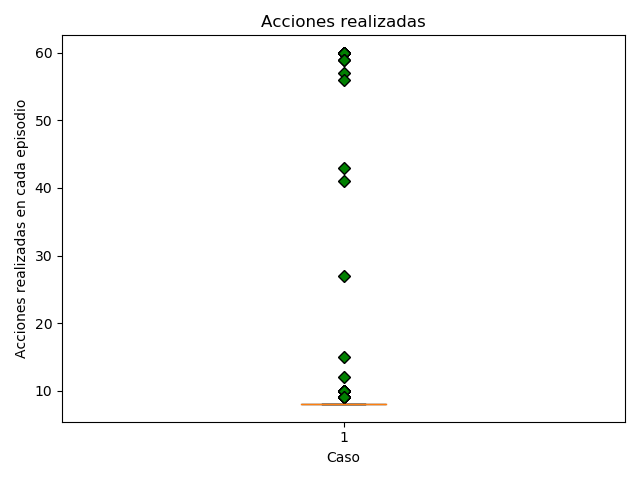
\includegraphics[scale=0.4]{cap5_experimentacion/images/dim5_lr0.01_ep0.2_boxplot.png}
    \caption{Boxplot del experimento \texttt{EPS3\_ER3}.}
    \label{fig:dim5_lr0.01_ep0.2_boxplot_EPS2_ER3}
\end{figure}

La secuencia de acciones aplicada se muestra en la  Fig.~\ref{fig:dim5_lr0.01_ep0.2_EPS2_ER3}. Se ha aplicado en 458 episodios de 500. 

\begin{figure}
    \centering
    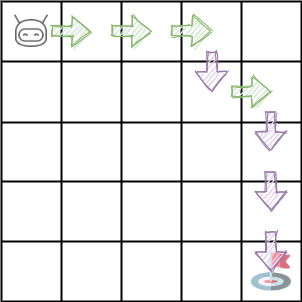
\includegraphics[scale=0.4]{cap5_experimentacion/images/dim5_lr0.01_ep0.2_458.png}
    \caption{Secuencia de acciones encontrada en el experimento \texttt{EPS3\_ER3}. Aplicada 458 veces.}
    \label{fig:dim5_lr0.01_ep0.2_EPS2_ER3}
\end{figure}

\paragraph{Análisis de las recompensas obtenidas y total de episodios resueltos} 

En cuanto a las recompensas, tal como se observa en la Fig.~\ref{fig:dim5_lr0.01_ep0.2_recompensa_EPS3_ER3} se han obtenido valores máximos a lo largo de la ejecución y con un número de penalizaciones bajo. \\
\begin{figure}
    \centering
    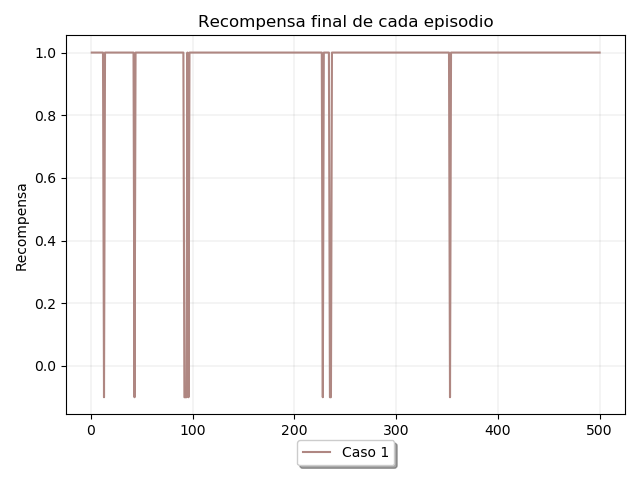
\includegraphics[scale=0.4]{cap5_experimentacion/images/dim5_lr0.01_ep0.2_recompensa.png}
    \caption{Recompensas finales de cada episodio del experimento \texttt{EPS3\_ER3}.}
    \label{fig:dim5_lr0.01_ep0.2_recompensa_EPS3_ER3}
\end{figure}

En este experimento de 500 episodios el agente ha sido capaz de alcanzar el objetivo en 490 episodios. En la Fig.~\ref{fig:dim5_lr0.01_ep0.2_porcentajeResuelto} se muestran los porcentajes de episodios resueltos y no resueltos del experimento. 

\begin{figure}
    \centering
    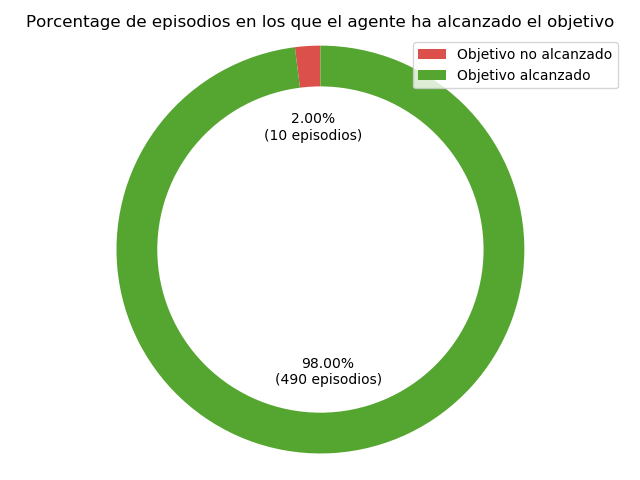
\includegraphics[scale=0.4]{cap5_experimentacion/images/dim5_lr0.01_ep0.2_porcentajeResuelto.png}
    \caption{Porcentaje de episodios en los que el agente alcanza el objetivo en el experimento \texttt{EPS3\_ER3}.}
    \label{fig:dim5_lr0.01_ep0.2_porcentajeResuelto}
\end{figure}

\subsubsection{EPS3\_ER4: Exploration rate 0.3} \label{EPS2_ER4}

En este experimento el \textit{exploration rate} es de 0.3, de modo que se explora el entorno el 30\% de las veces y el 70\% restante se emplean los conocimientos ya adquiridos.

\paragraph{Análisis de las acciones realizadas}

La Fig.~\ref{fig:dim5_lr0.01_ep0.3_acciones} muestra que las acciones realizadas a lo largo del experimento no se han estabilizado por completo, alternando el valor entre óptimo (8) y el máximo (60). \\

\begin{figure}
    \centering
    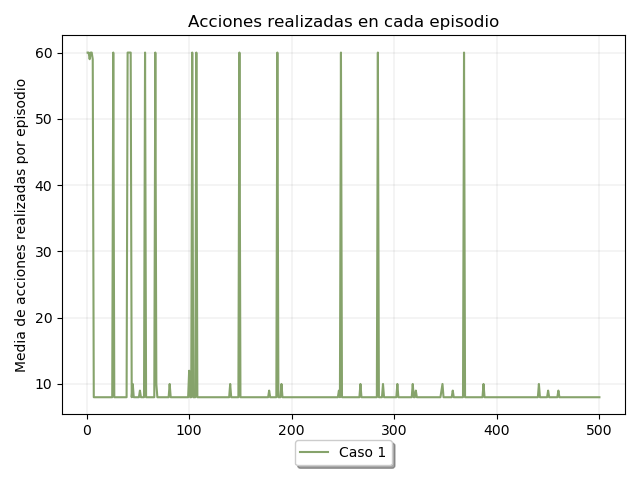
\includegraphics[scale=0.4]{cap5_experimentacion/images/dim5_lr0.01_ep0.3_acciones.png}
    \caption{Acciones realizadas por episodio en el experimento \texttt{EPS3\_ER4}.}
    \label{fig:dim5_lr0.01_ep0.3_acciones}
\end{figure}

Sin embargo, en el boxplot de la Fig.~\ref{fig:dim5_lr0.01_ep0.3_boxplot} se muestra que la media de la distribución de los datos es igual al número de acciones óptimo, por lo que parece que se ha estabilizado el total de acciones realizadas. \\

\begin{figure}
    \centering
    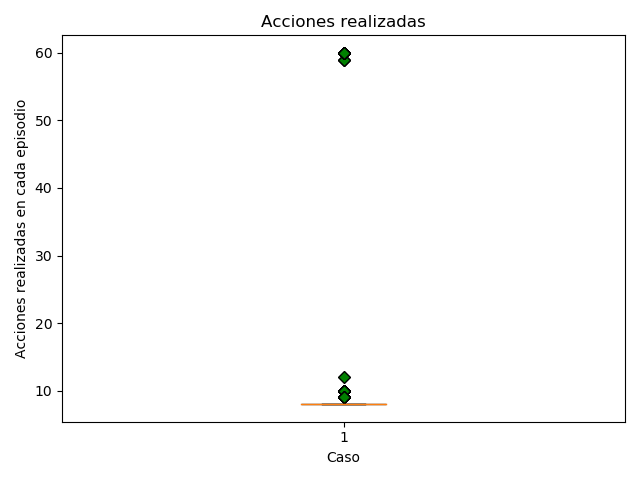
\includegraphics[scale=0.4]{cap5_experimentacion/images/dim5_lr0.01_ep0.3_boxplot.png}
    \caption{Boxplot del experimento \texttt{EPS3\_ER4}.}
    \label{fig:dim5_lr0.01_ep0.3_boxplot}
\end{figure}

En este experimento se han encontrado 2 secuencias de acciones diferentes: la predominante se ha aplicado 409 veces y se muestra en la Fig.~\ref{fig:dim5_lr0.01_ep0.3_409}; la segunda se ha aplicado 47 veces y se muestra en la Fig.~\ref{fig:dim5_lr0.01_ep0.3_47}. En total se ha alcanzado un número de episodios resueltos similar a los anteriores (456 episodios resueltos de 500).

\begin{figure}
    \centering
    \begin{subfigure}{.5\textwidth}
        \centering
        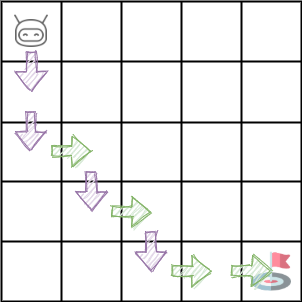
\includegraphics[scale=0.4]{cap5_experimentacion/images/dim5_lr0.01_ep0.3_409.png}
        \caption{Aplicada 409 veces.}
        \label{fig:dim5_lr0.01_ep0.3_409}
    \end{subfigure}%       
    \begin{subfigure}{.5\textwidth}
        \centering
        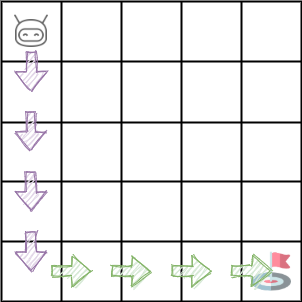
\includegraphics[scale=0.4]{cap5_experimentacion/images/dim5_lr0.01_ep0.3_47.png}
        \caption{Aplicada 47 veces.}
        \label{fig:dim5_lr0.01_ep0.3_47}
    \end{subfigure}
    \caption{Secuencias de acciones encontradas en el experimento \texttt{EPS3\_ER4}.}
    \label{fig:dim5_lr0.01_ep0.3}
\end{figure}

\paragraph{Análisis de las recompensas obtenidas y total de episodios resueltos} 

En cuanto a las recompensas, tal como se observa en la Fig.~\ref{fig:dim5_lr0.01_ep0.3_recompensa} se han obtenido valores máximos a lo largo de la ejecución y con un número de penalizaciones medio pero aceptables. Hay que recordar que es normal que el agente cometa algún error ya que aún está aprendiendo. \\

\begin{figure}
    \centering
    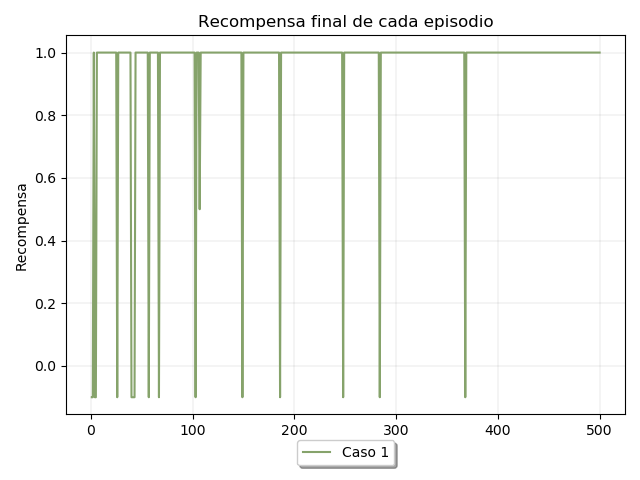
\includegraphics[scale=0.4]{cap5_experimentacion/images/dim5_lr0.01_ep0.3_recompensa.png}
    \caption{Recompensas finales de cada episodio del experimento \texttt{EPS3\_ER4}.}
    \label{fig:dim5_lr0.01_ep0.3_recompensa}
\end{figure}

En este experimento de 500 episodios el agente ha sido capaz de alcanzar el objetivo en 482 episodios. En la Fig.~\ref{fig:dim5_lr0.01_ep0.3_porcentajeResuelto} se muestran los porcentajes de episodios resueltos y no resueltos del experimento.

\begin{figure}
    \centering
    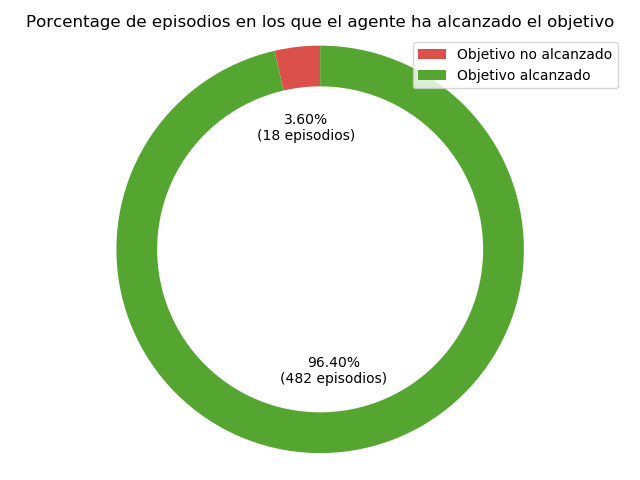
\includegraphics[scale=0.4]{cap5_experimentacion/images/dim5_lr0.01_ep0.3_porcentajeResuelto.png}
    \caption{Porcentaje de episodios en los que el agente alcanza el objetivo en el experimento \texttt{EPS3\_ER4}.}
    \label{fig:dim5_lr0.01_ep0.3_porcentajeResuelto}
\end{figure}

\subsubsection{EPS3\_ER5: Exploration rate 0.4} \label{EPS3_ER5}

En este experimento el \textit{exploration rate} es de 0.4, de modo que se explora el entorno el 40\% de las veces y el 60\% restante se emplean los conocimientos ya adquiridos. \\

\paragraph{Análisis de las acciones realizadas}

Las acciones realizadas en cada episodio se estabilizan en el valor máximo permitido, tal como se observa en la Fig.~\ref{fig:dim5_lr0.01_ep0.4_acciones}. \\

\begin{figure}
    \centering
    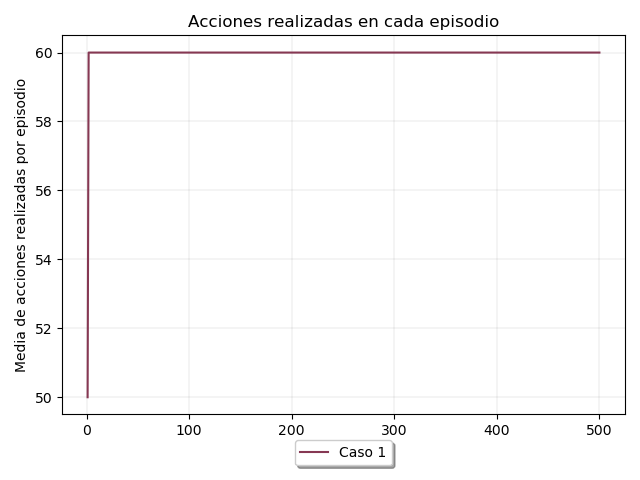
\includegraphics[scale=0.4]{cap5_experimentacion/images/dim5_lr0.01_ep0.4_acciones.png}
    \caption{Acciones realizadas por episodio en el experimento \texttt{EPS3\_ER5}.}
    \label{fig:dim5_lr0.01_ep0.4_acciones}
\end{figure}

En el boxplot de la Fig.~\ref{fig:dim5_lr0.01_ep0.4_boxplot} se observa que la media de las acciones realizada tiene el valor 60, el número máximo de acciones permitidas. \\

\begin{figure}
    \centering
    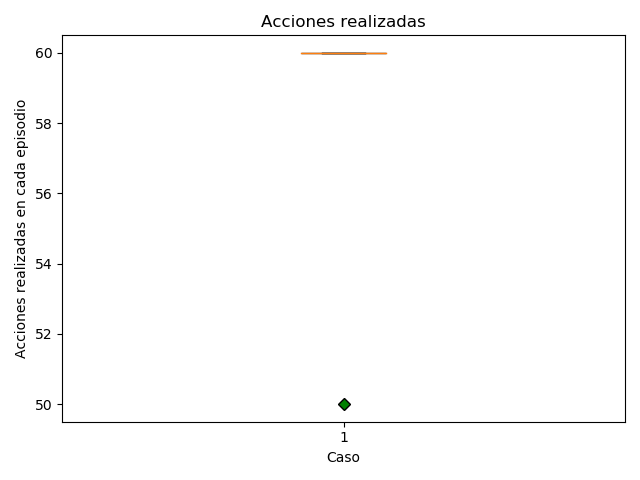
\includegraphics[scale=0.4]{cap5_experimentacion/images/dim5_lr0.01_ep0.4_boxplot.png}
    \caption{Boxplot del experimento \texttt{EPS3\_ER5}.}
    \label{fig:dim5_lr0.01_ep0.4_boxplot}
\end{figure}

En cuanto a las secuencias de acciones, no se ha encontrado ninguna que permita al agente alcanzar el objetivo. 

\paragraph{Análisis de las recompensas obtenidas y total de episodios resueltos} 

La recompensa obtenida a lo largo del experimento se encuentra por debajo del cero y, además, se le ha penalizado el agente en episodios consecutivos. En la Fig.~\ref{fig:dim5_lr0.01_ep0.4_recompensa} se aprecian dichas recompensas. \\

\begin{figure}
    \centering
    \includegraphics[scale=0.4]{cap5_experimentacion/images/dim5_lr0.01_ep0.4_recompensa.png}
    \caption{Recompensas finales de cada episodio del experimento \texttt{EPS3\_ER5}.}
    \label{fig:dim5_lr0.01_ep0.4_recompensa}
\end{figure}

En este experimento de 500 episodios el agente ha sido capaz de alcanzar el objetivo en un sólo episodio. En la Fig.~\ref{fig:dim5_lr0.01_ep0.4_porcentajeResuelto} se muestran los porcentajes de episodios resueltos y no resueltos del experimento. 

\begin{figure}
    \centering
    \includegraphics[scale=0.4]{cap5_experimentacion/images/dim5_lr0.01_ep0.4_porcentajeResuelto.png}
    \caption{Porcentaje de episodios en los que el agente alcanza el objetivo en el experimento \texttt{EPS3\_ER5}.}
    \label{fig:dim5_lr0.01_ep0.4_porcentajeResuelto}
\end{figure}

\subsubsection{EPS3\_ER6: Exploration rate 0.5} \label{EPS3_ER6}

En este experimento el \textit{exploration rate} es de 0.5, de modo que se explora el entorno la mitad de las veces y la otra mitad restante se emplean los conocimientos ya adquiridos. \\

\paragraph{Análisis de las acciones realizadas}

En la Fig.~\ref{fig:dim5_lr0.01_ep0.5_acciones} se muestra el número total de acciones por episodio realizado a lo largo del experimento. Dichas acciones se estabilizan en el valor máximo permitido, teniendo en el inicio del experimento unos episodios en los que sí que se ha alcanzado el valor óptimo. \\

\begin{figure}
    \centering
    \includegraphics[scale=0.4]{cap5_experimentacion/images/dim5_lr0.01_ep0.5_acciones.png}
    \caption{Acciones realizadas por episodio en el experimento \texttt{EPS3\_ER6}.}
    \label{fig:dim5_lr0.01_ep0.5_acciones}
\end{figure}

El boxplot de la Fig.~\ref{fig:dim5_lr0.01_ep0.5_boxplot} muestra que la media de las acciones realizadas es de 60 acciones. \\
\begin{figure}
    \centering
    \includegraphics[scale=0.4]{cap5_experimentacion/images/dim5_lr0.01_ep0.5_boxplot.png}
    \caption{Boxplot del experimento \texttt{EPS3\_ER6}.}
    \label{fig:dim5_lr0.01_ep0.5_boxplot}
\end{figure}

Aunque haya tenido tan malos resultados, el agente ha sido capaz de alcanzar su objetivo siguiendo 2 secuencias de acciones. Dichas secuencias se muestran en la Fig.~\ref{fig:dim5_lr0.01_ep0.5_6}. Ambas se han aplicado en 6 episodios distintos del experimento.  \\ 
\begin{figure}
    \centering
    \begin{subfigure}{.5\textwidth}
        \centering
        \includegraphics[scale=0.4]{cap5_experimentacion/images/dim5_lr0.01_ep0.5_6_1.png}
        \caption{Aplicada 6 veces.}
        \label{fig:dim5_lr0.01_ep0.5_6_1}
    \end{subfigure}%       
    \begin{subfigure}{.5\textwidth}
        \centering
        \includegraphics[scale=0.4]{cap5_experimentacion/images/dim5_lr0.01_ep0.5_6_2.png}
        \caption{Aplicada 6 veces.}
        \label{fig:dim5_lr0.01_ep0.5_6_2}
    \end{subfigure}
    \caption{Secuencias de acciones seguidas en el experimento \texttt{EPS3\_ER6}.}
    \label{fig:dim5_lr0.01_ep0.5_6}
\end{figure}

\paragraph{Análisis de las recompensas obtenidas y total de episodios resueltos} 

Sin embargo, como bien se ha mencionado anteriormente, al principio del experimento el agente ha recibido recompensas máximas en varios episodios. El resto del experimento recibe penalizaciones, pero son menos frecuentes que en el experimento \nameref{EPS3_ER5}. \\

\begin{figure}
    \centering
    \includegraphics[scale=0.4]{cap5_experimentacion/images/dim5_lr0.01_ep0.5_recompensa.png}
    \caption{Recompensas finales de cada episodio del experimento \texttt{EPS3\_ER6}.}
    \label{fig:dim5_lr0.01_ep0.5_recompensa}
\end{figure}

En este experimento de 500 episodios el agente ha sido capaz de alcanzar el objetivo en 21 episodios. En la Fig.~\ref{fig:dim5_lr0.01_ep0.5_porcentajeResuelto} se muestran los porcentajes de episodios resueltos y no resueltos del experimento.

\begin{figure}
    \centering
    \includegraphics[scale=0.4]{cap5_experimentacion/images/dim5_lr0.01_ep0.5_porcentajeResuelto.png}
    \caption{Porcentaje de episodios en los que el agente alcanza el objetivo en el experimento \texttt{EPS3\_ER6}.}
    \label{fig:dim5_lr0.01_ep0.5_porcentajeResuelto}
\end{figure}

\subsubsection{EPS3\_ER7: Exploration rate 0.6} \label{EPS3_ER7}

En este experimento el \textit{exploration rate} es de 0.6, de modo que se explora el 60\% las veces y en el 40\% restante se emplean los conocimientos ya adquiridos. \\

\paragraph{Análisis de las acciones realizadas}

El total de acciones realizadas vuelven a estabilizarse en el valor máximo permitido tal como se muestra en la Fig.~\ref{fig:dim5_lr0.01_ep0.6_acciones}. \\

\begin{figure}
    \centering
    \includegraphics[scale=0.4]{cap5_experimentacion/images/dim5_lr0.01_ep0.6_acciones.png}
    \caption{Acciones realizadas por episodio en el experimento \texttt{EPS3\_ER7}.}
    \label{fig:dim5_lr0.01_ep0.6_acciones}
\end{figure}

En la Fig.~\ref{fig:dim5_lr0.01_ep0.6_boxplot} se muestra que la media de acciones es de 60. \\ 

\begin{figure}
    \centering
    \includegraphics[scale=0.4]{cap5_experimentacion/images/dim5_lr0.01_ep0.6_boxplot.png}
    \caption{Boxplot del experimento \texttt{EPS3\_ER7}.}
    \label{fig:dim5_lr0.01_ep0.6_boxplot}
\end{figure}

No se ha encontrado ninguna secuencia de acciones que lleven al agente al objetivo.

\paragraph{Análisis de las recompensas obtenidas y total de episodios resueltos} 

En cuanto a las recompensas mostradas en la Fig.~\ref{fig:dim5_lr0.01_ep0.6_recompensa}, se puede decir que son las peores recompensas que se han obtenido de todos los experimentos realizados ya que las penalizaciones son secuenciales casi en la totalidad de los episodios. \\

\begin{figure}
    \centering
    \includegraphics[scale=0.4]{cap5_experimentacion/images/dim5_lr0.01_ep0.6_recompensa.png}
    \caption{Recompensas finales de cada episodio del experimento \texttt{EPS3\_ER7}.}
    \label{fig:dim5_lr0.01_ep0.6_recompensa}
\end{figure}

En este experimento de 500 episodios el agente no ha sido capaz de alcanzar el objetivo tal como se muestra en la Fig.~\ref{fig:dim5_lr0.01_ep0.6_porcentajeResuelto}.

\begin{figure}
    \centering
    \includegraphics[scale=0.4]{cap5_experimentacion/images/dim5_lr0.01_ep0.6_porcentajeResuelto.png}
    \caption{Porcentaje de episodios en los que el agente alcanza el objetivo en el experimento \texttt{EPS3\_ER7}.}
    \label{fig:dim5_lr0.01_ep0.6_porcentajeResuelto}
\end{figure}

\subsubsection{EPS3\_ER8: Exploration rate 0.7} \label{EPS2_ER8}

En este experimento el \textit{exploration rate} es de 0.7, de modo que se explora el 70\% las veces y en el 30\% restante se emplean los conocimientos ya adquiridos. \\

\paragraph{Análisis de acciones realizadas}

La Fig.~\ref{fig:dim5_lr0.01_ep0.7_acciones} muestra las acciones realizadas en cada episodio; respecto a los experimentos anteriores, se puede observar que los resultados obtenidos en este experimento son los mejores, ya que el número total de acciones realizadas en los episodios son estables entorno al valor óptimo. \\

\begin{figure}
    \centering
    \includegraphics[scale=0.4]{cap5_experimentacion/images/dim5_lr0.01_ep0.7_acciones.png}
    \caption{Acciones realizadas por episodio en el experimento \texttt{EPS3\_ER8}.}
    \label{fig:dim5_lr0.01_ep0.7_acciones}
\end{figure}

El boxplot de la Fig.~\ref{fig:dim5_lr0.01_ep0.7_boxplot} nos muestra que, además, el total de acciones tomadas en cada episodio a lo largo de la ejecución tiene una media de 8. \\

\begin{figure}
    \centering
    \includegraphics[scale=0.4]{cap5_experimentacion/images/dim5_lr0.01_ep0.7_boxplot.png}
    \caption{Boxplot del experimento \texttt{EPS3\_ER8}.}
    \label{fig:dim5_lr0.01_ep0.7_boxplot}
\end{figure}

En este experimento se han encontrado 6 secuencias distintas de acciones que se han realizado para alcanzar el objetivo. La secuencia predominante es la que se muestra en la Fig.~\ref{fig:dim5_lr0.01_ep0.7_174}, con un total de 174 episodios en los que se ha aplicado. \\
\begin{figure}
    \centering
    \begin{subfigure}{.3\textwidth}
        \centering
        \includegraphics[scale=0.35]{cap5_experimentacion/images/dim5_lr0.01_ep0.7_174.png}
        \caption{Aplicada 174 veces.}
        \label{fig:dim5_lr0.01_ep0.7_174}
    \end{subfigure}%       
    \begin{subfigure}{.3\textwidth}
        \centering
        \includegraphics[scale=0.35]{cap5_experimentacion/images/dim5_lr0.01_ep0.7_139.png}
        \caption{Aplicada 139 veces.}
        \label{fig:dim5_lr0.01_ep0.7_139}
    \end{subfigure}%
    \begin{subfigure}{.3\textwidth}
        \centering
        \includegraphics[scale=0.35]{cap5_experimentacion/images/dim5_lr0.01_ep0.7_88.png}
        \caption{Aplicada 88 veces.}
        \label{fig:dim5_lr0.01_ep0.7_88}
    \end{subfigure}
    \begin{subfigure}{.3\textwidth}
        \centering
        \includegraphics[scale=0.35]{cap5_experimentacion/images/dim5_lr0.01_ep0.7_32.png}
        \caption{Aplicada 32 veces.}
        \label{fig:dim5_lr0.01_ep0.7_32}
    \end{subfigure}%       
    \begin{subfigure}{.3\textwidth}
        \centering
        \includegraphics[scale=0.35]{cap5_experimentacion/images/dim5_lr0.01_ep0.7_30.png}
        \caption{Aplicada 30 veces.}
        \label{fig:dim5_lr0.01_ep0.7_30}
    \end{subfigure}%
    \begin{subfigure}{.3\textwidth}
        \centering
        \includegraphics[scale=0.35]{cap5_experimentacion/images/dim5_lr0.01_ep0.7_7.png}
        \caption{Aplicada 7 veces.}
        \label{fig:dim5_lr0.01_ep0.7_7}
    \end{subfigure}
    \caption{Secuencias de acciones seguidas en el experimento \texttt{EPS3\_ER8}}
    \label{fig:dim5_lr0.01_ep0.7}
\end{figure}


\paragraph{Análisis de las recompensas obtenidas y total de episodios resueltos} 

En cuanto a la recompensa mostrada en la Fig.~\ref{fig:dim5_lr0.01_ep0.7_recompensa}, se observa que es máxima a lo largo de toda la ejecución con la excepción de una única penalización recibida. \\

\begin{figure}
    \centering
    \includegraphics[scale=0.4]{cap5_experimentacion/images/dim5_lr0.01_ep0.7_recompensa.png}
    \caption{Recompensas finales de cada episodio del experimento \texttt{EPS3\_ER8}.}
    \label{fig:dim5_lr0.01_ep0.7_recompensa}
\end{figure}

En este experimento de 500 episodios el agente ha sido capaz de alcanzar el objetivo en 496 episodios. En la Fig.~\ref{fig:dim5_lr0.01_ep0.7_porcentajeResuelto} se muestran los porcentajes de episodios resueltos y no resueltos del experimento. 

\begin{figure}
    \centering
    \includegraphics[scale=0.4]{cap5_experimentacion/images/dim5_lr0.01_ep0.7_porcentajeResuelto.png}
    \caption{Porcentaje de episodios en los que el agente alcanza el objetivo en el experimento \texttt{EPS3\_ER8}.}
    \label{fig:dim5_lr0.01_ep0.7_porcentajeResuelto}
\end{figure}

\subsubsection{EPS3\_ER9: Exploration rate 0.8} \label{EPS2_ER9}

En este experimento el \textit{exploration rate} es de 0.8, de modo que se explora el 80\% las veces y en el 20\% restante se emplean los conocimientos ya adquiridos. \\

\paragraph{Análisis de las acciones realizadas}

En este experimento el total de acciones realizadas vuelven a estabilizarse en el valor máximo permitido. En la Fig.~\ref{fig:dim5_lr0.01_ep0.8_acciones} se aprecia la evolución a lo largo del experimento. \\

\begin{figure}
    \centering
    \includegraphics[scale=0.4]{cap5_experimentacion/images/dim5_lr0.01_ep0.8_acciones.png}
        \caption{Acciones realizadas por episodio en el experimento \texttt{EPS3\_ER9}.}
    \label{fig:dim5_lr0.01_ep0.8_acciones}
\end{figure}

En el boxplot de la Fig.~\ref{fig:dim5_lr0.01_ep0.8_boxplot} se puede ver que la media de las acciones realizadas es de 60.

\begin{figure}
    \centering
    \includegraphics[scale=0.4]{cap5_experimentacion/images/dim5_lr0.01_ep0.8_boxplot.png}
    \caption{Boxplot del experimento \texttt{EPS3\_ER9}.}
    \label{fig:dim5_lr0.01_ep0.8_boxplot}
\end{figure}

\paragraph{Análisis de las recompensas obtenidas y total de episodios resueltos} 

Las recompensas, mostradas en la la Fig.~\ref{fig:dim5_lr0.01_ep0.8_recompensa}, han sido mayoritariamente negativas. \\

\begin{figure}
    \centering
    \includegraphics[scale=0.4]{cap5_experimentacion/images/dim5_lr0.01_ep0.8_recompensa.png}
    \caption{Recompensas finales de cada episodio del experimento \texttt{EPS3\_ER9}.}
    \label{fig:dim5_lr0.01_ep0.8_recompensa}
\end{figure}

En este experimento de 500 episodios el agente ha sido capaz de alcanzar el objetivo en un único episodio, tal como se aprecia en la Fig.~\ref{fig:dim5_lr0.01_ep0.8_porcentajeResuelto}. 

\begin{figure}
    \centering
    \includegraphics[scale=0.4]{cap5_experimentacion/images/dim5_lr0.01_ep0.8_porcentajeResuelto.png}
    \caption{Porcentaje de episodios en los que el agente alcanza el objetivo en el experimento \texttt{EPS3\_ER9}.}
    \label{fig:dim5_lr0.01_ep0.8_porcentajeResuelto}
\end{figure}

\subsubsection{EPS3\_ER10: Exploration rate 0.9}

En este experimento el \textit{exploration rate} es de 0.9, de modo que se explora el 90\% las veces y en el 10\% restante se emplean los conocimientos ya adquiridos.

\paragraph{Análisis de las acciones realizadas}

La Fig.~\ref{fig:dim5_lr0.01_ep0.9_acciones} muestra las acciones realizadas en cada episodio. El número de acciones realizados por episodio se ha estabilizado en el valor óptimo. \\

\begin{figure}
    \centering
    \includegraphics[scale=0.4]{cap5_experimentacion/images/dim5_lr0.01_ep0.9_acciones.png}
    \caption{Acciones realizadas por episodio en el experimento \texttt{EPS3\_ER10}.}
    \label{fig:dim5_lr0.01_ep0.9_acciones}
\end{figure}

El boxplot de la Fig.~\ref{fig:dim5_lr0.01_ep0.9_boxplot} muestra que la media es equivalente al valor óptimo, es decir, a 8. \\

\begin{figure}
    \centering
    \includegraphics[scale=0.4]{cap5_experimentacion/images/dim5_lr0.01_ep0.9_boxplot.png}
    \caption{Boxplot del experimento \texttt{EPS3\_ER10}.}
    \label{fig:dim5_lr0.01_ep0.9_boxplot}
\end{figure}
 
Se han encontrado 3 secuencias de acciones y se muestran en la Fig.~\ref{fig:dim5_lr0.01_ep0.9}. La secuencia predominante (Fig.~\ref{fig:dim5_lr0.01_ep0.9_383})se ha aplicado 383 veces. \\

\begin{figure}
    \centering
    \begin{subfigure}{.3\textwidth}
        \centering
        \includegraphics[scale=0.35]{cap5_experimentacion/images/dim5_lr0.01_ep0.9_383.png}
        \caption{Aplicada 383 veces.}
        \label{fig:dim5_lr0.01_ep0.9_383}
    \end{subfigure}%       
    \begin{subfigure}{.3\textwidth}
        \centering
        \includegraphics[scale=0.35]{cap5_experimentacion/images/dim5_lr0.01_ep0.9_55.png}
        \caption{Aplicada 55 veces.}
        \label{fig:dim5_lr0.01_ep0.9_55}
    \end{subfigure}%
    \begin{subfigure}{.3\textwidth}
        \centering
        \includegraphics[scale=0.35]{cap5_experimentacion/images/dim5_lr0.01_ep0.9_9.png}
        \caption{Aplicada 9 veces.}
        \label{fig:dim5_lr0.01_ep0.9_9}
    \end{subfigure}
    \caption{Secuencias de acciones seguidas en el experimento \texttt{EPS3\_ER10}.}
    \label{fig:dim5_lr0.01_ep0.9}
\end{figure}

\paragraph{Análisis de las recompensas obtenidas y total de episodios resueltos} 
 
En cuanto a las recompensas, tal como se muestran en la Fig.~\ref{fig:dim5_lr0.01_ep0.9_recompensa}, han sido máximas a lo largo del experimento menos en unos pocos episodios en los que el agente ha recibido recompensas negativas. \\
 
\begin{figure}
    \centering
    \includegraphics[scale=0.4]{cap5_experimentacion/images/dim5_lr0.01_ep0.9_recompensa.png}
    \caption{Recompensas finales de cada episodio del experimento \texttt{EPS3\_ER10}.}
    \label{fig:dim5_lr0.01_ep0.9_recompensa}
\end{figure}

En este experimento de 500 episodios, el agente ha sido capaz de alcanzar el objetivo en 481 episodios. En la Fig.~\ref{fig:dim5_lr0.01_ep0.9_porcentajeResuelto} se muestran los porcentajes de episodios resueltos y no resueltos del experimento. \\

\begin{figure}
    \centering
    \includegraphics[scale=0.4]{cap5_experimentacion/images/dim5_lr0.01_ep0.9_porcentajeResuelto.png}
    \caption{Porcentaje de episodios en los que el agente alcanza el objetivo en el experimento \texttt{EPS3\_ER10}.}
    \label{fig:dim5_lr0.01_ep0.9_porcentajeResuelto}
\end{figure}

\subsubsection{EPS3\_ER11: Exploration rate 1}

Y, por último, en este experimento el \textit{exploration rate} es de 1, de modo que se explora siempre el entorno y no se emplea nunca el conocimiento adquirido de las experiencias anteriores. 

\paragraph{Análisis de las acciones realizadas}

La Fig.~\ref{fig:dim5_lr0.01_ep1_acciones} muestra que las acciones realizadas a lo largo de la ejecución han sido relativamente estables alrededor del valor óptimo (8).\\

\begin{figure}
    \centering
    \includegraphics[scale=0.4]{cap5_experimentacion/images/dim5_lr0.01_ep1_acciones.png}
    \caption{Acciones realizadas por episodio en el experimento \texttt{EPS3\_ER11}.}
    \label{fig:dim5_lr0.01_ep1_acciones}
\end{figure}

El boxplot de la Fig.~\ref{fig:dim5_lr0.01_ep1_boxplot} muestra que la media es equivalente al valor óptimo, es decir, a 8. \\

\begin{figure}
    \centering
    \includegraphics[scale=0.4]{cap5_experimentacion/images/dim5_lr0.01_ep1_boxplot.png}
    \caption{Boxplot del experimento \texttt{EPS3\_ER11}.}
    \label{fig:dim5_lr0.01_ep1_boxplot}
\end{figure}

Se han encontrado 4 secuencias de acciones diferentes para alcanzar el objetivo. Se muestran en la Fig.~\ref{fig:dim5_lr0.01_ep1}.

\begin{figure}
    \centering
    \begin{subfigure}{.5\textwidth}
        \centering
        \includegraphics[scale=0.4]{cap5_experimentacion/images/dim5_lr0.01_ep1_203.png}
        \caption{Aplicada 203 veces.}
        \label{fig:dim5_lr0.01_ep1_203}
    \end{subfigure}%       
    \begin{subfigure}{.5\textwidth}
        \centering
        \includegraphics[scale=0.4]{cap5_experimentacion/images/dim5_lr0.01_ep1_153.png}
        \caption{Aplicada 153 veces.}
        \label{fig:dim5_lr0.01_ep1_153}
    \end{subfigure}
    \begin{subfigure}{.5\textwidth}
        \centering
        \includegraphics[scale=0.4]{cap5_experimentacion/images/dim5_lr0.01_ep1_51.png}
        \caption{Aplicada 51 veces.}
        \label{fig:dim5_lr0.01_ep1_51}
    \end{subfigure}%       
    \begin{subfigure}{.5\textwidth}
        \centering
        \includegraphics[scale=0.4]{cap5_experimentacion/images/dim5_lr0.01_ep1_43.png}
        \caption{Aplicada 43 veces.}
        \label{fig:dim5_lr0.01_ep1_43}
    \end{subfigure}
    \caption{Secuencias de acciones seguidas en el experimento \texttt{EPS3\_ER11}.}
    \label{fig:dim5_lr0.01_ep1}
\end{figure}

\paragraph{Análisis de las recompensas obtenidas y total de episodios resueltos} 

En cuanto a las recompensas, tal como se muestran en la Fig.~\ref{fig:dim5_lr0.01_ep1_recompensa}, han sido máximas a lo largo del experimento menos en unos pocos episodios en los que el agente ha recibido una penalización. \\
  
\begin{figure}
    \centering
    \includegraphics[scale=0.4]{cap5_experimentacion/images/dim5_lr0.01_ep1_recompensa.png}
    \caption{Recompensas finales de cada episodio del experimento \texttt{EPS3\_ER11}.}
    \label{fig:dim5_lr0.01_ep1_recompensa}
\end{figure}

En este experimento de 500 episodios, el agente ha sido capaz de alcanzar el objetivo en 485 episodios. En la Fig.~\ref{fig:dim5_lr0.01_ep1_porcentajeResuelto} se muestran los porcentajes de episodios resueltos y no resueltos del experimento. 

\begin{figure}
    \centering
    \includegraphics[scale=0.4]{cap5_experimentacion/images/dim5_lr0.01_ep1_porcentajeResuelto.png}
    \caption{Porcentaje de episodios en los que el agente alcanza el objetivo en el experimento \texttt{EPS3\_ER11}.}
    \label{fig:dim5_lr0.01_ep1_porcentajeResuelto}
\end{figure}

\subsection{CHG\_ORG: Alternando el inicio del agente en un entorno 5x5} \label{CHG_ORG}

Este experimento se ha separado en dos partes diferentes: en la primera parte se realiza la ejecución original y, en la segunda, se aplican variaciones en la configuración del entorno para observar si los resultados obtenidos cambian respecto a los resultados de la ejecución original. 

\subsubsection{Experimento original}

Este experimento se ha realizado con 3 iteraciones de 300 episodios cada. Las posición inicial del agente se ha ido variando y la del posición del objetivo ha sido en (4, 4). Se ha empleado el modelo del agente obtenido en el experimento anterior \nameref{EPS1}, es decir, la red está ajustada con los pesos obtenidos a partir de la realización de este experimento en concreto. \\


En la Fig.~\ref{fig:chg_org_config} se puede visualizar el entorno del problema con las configuraciones de cada iteración. \\

\begin{figure}
    \centering
    \begin{subfigure}{.35\textwidth}
        \centering
        \includegraphics[scale=0.35]{cap5_experimentacion/images/chg_org_it1.png}
        \caption{Para 1ª iteración.}
        \label{fig:chg_org_it1}
    \end{subfigure}%       
    \begin{subfigure}{.35\textwidth}
        \centering
        \includegraphics[scale=0.35]{cap5_experimentacion/images/chg_org_it2.png}
        \caption{Para la 2ª iteración.}
        \label{fig:chg_org_it2}
    \end{subfigure}%
    \begin{subfigure}{.35\textwidth}
        \centering
        \includegraphics[scale=0.35]{cap5_experimentacion/images/chg_org_it3.png}
        \caption{Para la 3ª iteración.}
        \label{fig:chg_org_it3}
    \end{subfigure}%       
    \caption{Configuraciones adoptadas en cada una de las iteraciones del experimento \texttt{CHG\_ORG}.}
    \label{fig:chg_org_config}
\end{figure}

En el experimento original, las posiciones iniciales del agente para cada iteración han sido: 

\begin{enumerate}
    \item En la 1ª iteración el agente estaba en (4, 2), teniendo así una distancia de 2 hasta el objetivo. La distancia óptima es de 2. La configuración es la mostrada en la Fig.~\ref{fig:chg_org_it1}.
    \item En la 2ª iteración el agente empezaba en (3, 0), teniendo así una distancia de 5 hasta el objetivo. La distancia óptima es de 5.  La configuración es la mostrada en la Fig.~\ref{fig:chg_org_it2}.
    \item En la 3ª iteración el agente empezaba en (2, 0), teniendo así una distancia de 6 hasta el objetivo. La distancia óptima es de 6.  La configuración es la mostrada en la Fig.~\ref{fig:chg_org_it3}.
\end{enumerate}

\paragraph{Análisis de las acciones realizadas}

Se puede observar en la Fig.~\ref{fig:CHANGE_ORIGIN-20-09_00-42-50_acciones} que para cada iteración: 
\begin{enumerate}
    \item En la 1ª iteración, el total de acciones realizadas se estabiliza en el valor óptimo (2 en este caso). 
    \item En la 2ª iteración el agente al principio realiza unas secuencias de acciones que no son óptimas y, además, hay mucha variación entre ellas. A partir del episodio 70 aproximadamente se comienza a estabilizar en su valor óptimo pero sigue teniendo picos altos a lo largo de la ejecución. 
    \item En la 3ª iteración el agente se estabiliza a partir del episodio 40 aproximadamente en su valor óptimo de acciones.  
\end{enumerate}

\begin{figure}
    \centering
    \includegraphics[scale=0.4]{cap5_experimentacion/images/CHANGE_ORIGIN-20-09_00-42-50_acciones.png}
    \caption{Acciones realizadas por episodio en el experimento \texttt{CHG\_ORG}.}
    \label{fig:CHANGE_ORIGIN-20-09_00-42-50_acciones}
\end{figure}

En cuanto a la distribución de los datos que se muestra en la Fig.~\ref{fig:CHANGE_ORIGIN-20-09_00-42-50_boxplot}, se puede comprobar que: 
\begin{enumerate}
    \item En la 1ª iteración la distribución de las acciones tiene como media el valor óptimo de acciones (2 en este caso). 
    \item En la 2ª iteración por otro lado, las acciones totales realizadas están en un rango entre el valor óptimo (6 en este caso) y 15 aproximadamente, por lo que no se ha estabilizado demasiado. La media sin embargo está en su valor óptimo, 6. 
    \item En la 3ª iteración, al igual que el la 1ª, los valores tienen como media el valor óptimo (5 en este caso).
\end{enumerate}

De este \textit{boxplot} se puede concluir que la 2ª iteración el la que peores resultados ofrece ya que los valores obtenidos varían mucho. \\

\begin{figure}
    \centering
    \includegraphics[scale=0.4]{cap5_experimentacion/images/CHANGE_ORIGIN-20-09_00-42-50_boxplot.png}
    \caption{Boxplot del experimento \texttt{CHG\_ORG}.}
    \label{fig:CHANGE_ORIGIN-20-09_00-42-50_boxplot}
\end{figure}

En la 1ª iteración la secuencia de acciones es sencilla, como se puede observar en la  Fig.~\ref{fig:dim5_CHANGE_ORIGIN-20-09_00-42-50}. De los 300 episodios, se ha aplicado 286 veces. Esto indica que el agente casi siempre ha llegado a la solución correcta y se ha equivocado muy pocas veces.\\

\begin{figure}
    \centering
    \includegraphics[scale=0.4]{cap5_experimentacion/images/dim5_CHANGE_ORIGIN-20-09_00-42-50.png}
    \caption{1ª iteración del experimento \texttt{CHG\_ORG}. Aplicada 286 veces.}
    \label{fig:dim5_CHANGE_ORIGIN-20-09_00-42-50}
\end{figure}

En la 2ª iteración, mostrada en la Fig.~\ref{fig:dim5_CHANGE_ORIGIN-20-09_00-42-50_213}, se ha encontrado una secuencia predominante que se ha aplicado 213 veces del total de 300 episodios realizados. \\

\begin{figure}
    \centering
    \includegraphics[scale=0.4]{cap5_experimentacion/images/dim5_CHANGE_ORIGIN-20-09_00-42-50_213.png}
    \caption{2ª iteración del experimento \texttt{CHG\_ORG}. Aplicada 213 veces.}
    \label{fig:dim5_CHANGE_ORIGIN-20-09_00-42-50_213}
\end{figure}

Por último, en la 3ª iteración mostrada en la Fig.~\ref{fig:dim5_CHANGE_ORIGIN-20-09_00-42-50_3iter} se han aplicado 2 secuencias distintas para alcanzar el objetivo. De hecho, dichas secuencias se han aplicado casi por igual, con la primera secuencia 155 veces realizada y la segunda 121 veces. La suma de las secuencias muestra que se 300 episodios se ha alcanzado una solución 276 veces.
 
\begin{figure}
    \centering
    \begin{subfigure}{.5\textwidth}
        \centering
        \includegraphics[scale=0.4]{cap5_experimentacion/images/dim5_CHANGE_ORIGIN-20-09_00-42-50_155.png}
        \caption{Aplicada 155 veces.}
        \label{fig:dim5_CHANGE_ORIGIN-20-09_00-42-50_155}
    \end{subfigure}%       
    \begin{subfigure}{.5\textwidth}
        \centering
        \includegraphics[scale=0.4]{cap5_experimentacion/images/dim5_CHANGE_ORIGIN-20-09_00-42-50_121.png}
        \caption{Aplicada 121 veces.}
        \label{fig:dim5_CHANGE_ORIGIN-20-09_00-42-50_121}
    \end{subfigure}
    \caption{3ª iteración del experimento \texttt{CHG\_ORG}.}
    \label{fig:dim5_CHANGE_ORIGIN-20-09_00-42-50_3iter}
\end{figure}

\paragraph{Análisis de las recompensas obtenidas y total de episodios resueltos} 

En cuanto a las recompensas obtenidas, se muestran en la Fig.~\ref{fig:CHANGE_ORIGIN-20-09_00-42-50_recompensa} y se puede observar que: 
\begin{enumerate}
    \item En la 1ª iteración la recompensa es siempre la máxima, menos en dos ocasiones que ha recibido penalizaciones.  
    \item En la 2ª iteración el agente recibe muchas penalizaciones.
    \item En la 3ª iteración se nos presenta el mismo caso que en la 1ª, recompensa máxima casi siempre y con pocas penalizaciones. Sin embargo, se puede observar que en varios episodios seguidos ha obtenido penalizaciones. Incluso realizando tantas malas acciones inicialmente, el agente ha conseguido alcanzar la máxima recompensa en el resto de la ejecución. 
\end{enumerate}

\begin{figure}
    \centering
    \includegraphics[scale=0.4]{cap5_experimentacion/images/CHANGE_ORIGIN-20-09_00-42-50_recompensa.png}
    \caption{Recompensas finales de cada episodio del experimento \texttt{CHG\_ORG}.}
    \label{fig:CHANGE_ORIGIN-20-09_00-42-50_recompensa}
\end{figure}

En cuanto al total de episodios resueltos en cada iteración, teniendo en cuenta de se han realizado 300 episodios, se puede observar que: 
\begin{enumerate}
    \item En la 1ª iteración se han resuelto 297 episodios, tal como se observa en Fig.~\ref{fig:chg_org_it1_porcentajeResuelto}.
    \item En la 2ª iteración se han resuelto 231 episodios, tal como se observa en Fig.~\ref{fig:chg_org_it2_porcentajeResuelto}.
    \item En la 3ª iteración se han resuelto 283 episodios, tal como se observa en Fig.~\ref{fig:chg_org_it3_porcentajeResuelto}.
\end{enumerate}

\begin{figure}
    \centering
    \begin{subfigure}{.5\textwidth}
        \centering
        \includegraphics[scale=0.3]{cap5_experimentacion/images/CHANGE_ORIGIN-20-09_00-42-50_it1_porcentajeResuelto.png}
        \caption{Para 1ª iteración.}
        \label{fig:chg_org_it1_porcentajeResuelto}
    \end{subfigure}%       
    \begin{subfigure}{.5\textwidth}
        \centering
        \includegraphics[scale=0.3]{cap5_experimentacion/images/CHANGE_ORIGIN-20-09_00-42-50_it2_porcentajeResuelto.png}
        \caption{Para la 2ª iteración.}
        \label{fig:chg_org_it2_porcentajeResuelto}
    \end{subfigure}
    \begin{subfigure}{.5\textwidth}
        \centering
        \includegraphics[scale=0.3]{cap5_experimentacion/images/CHANGE_ORIGIN-20-09_00-42-50_it3_porcentajeResuelto.png}
        \caption{Para la 3ª iteración.}
        \label{fig:chg_org_it3_porcentajeResuelto}
    \end{subfigure}%       
    \caption{Porcentaje de episodios en los que el agente alcanza el objetivo en el experimento \texttt{CHG\_ORG}.}
    \label{fig:CHANGE_ORIGIN-20-09_00-42-50_porcentajeResuelto}
\end{figure}

En conclusión, este experimento ha sido exitoso en 2 de las 3 iteraciones realizadas, ya que en la 2ª iteración el agente ha realizado demasiadas acciones incorrectas y cuando ha conseguido alcanzar el objetivo, el total de acciones realizadas cada episodio variaba mucho. En las dos iteraciones restantes se ha alcanzado una solución más robusta ya que el número de acciones no variaba demasiado y las recompensas obtenidas eran máximas en la mayoría de episodios. \\ 
 
A partir de este experimento se han realizado varias repeticiones del mismo pero permutando las distancias de cada iteración para observar si los resultados cambian. 

\subsubsection{REP\_CHG\_ORG1: Repetición experimento con orden 1, 3, 2} \label{REP_CHG_ORG1}

En esta repetición del experimento se ha seguido el siguiente orden: 
\begin{enumerate}
    \item La 1ª iteración se mantiene,  de modo que el agente está inicialmente en (4, 2) y teniendo una distancia de 2 hasta el objetivo. La distancia óptima es de 2. La configuración es la mostrada en la Fig.~\ref{fig:chg_org_it1}.
    \item La 2ª iteración se corresponde con la iteración 3 del experimento original, de modo que el agente está inicialmente en (2, 0) y teniendo una distancia de 6 hasta el objetivo. La distancia óptima es de 6. La configuración es la mostrada en la Fig.~\ref{fig:chg_org_it3}.
    \item La 3ª iteración se corresponde con la iteración 2 del experimento original, de modo que el agente está inicialmente en (3, 0) y teniendo una distancia de 5 hasta el objetivo. La distancia óptima es de 5. La configuración es la mostrada en la Fig.~\ref{fig:chg_org_it2}.
\end{enumerate}

\paragraph{Análisis de las acciones realizadas}

Se puede observar en la Fig.~\ref{fig:CHANGE_ORIGIN-20_09-00_50-0, 2, 1_acciones} que para cada iteración: 
\begin{enumerate}
    \item En la 1ª iteración, el total de acciones realizadas se estabiliza en el valor óptimo (2 en este caso). 
    \item En la 2ª iteración el agente al principio realiza unas secuencias de acciones que no son óptimas y, además, hay mucha variación entre ellas. A partir del episodio 70 aproximadamente se comienza a estabilizar en su valor óptimo y tiene pocos picos altos en el resto de la ejecución. 
    \item En la 3ª iteración el agente realiza un número óptimo de acciones y la evolución es estable, menos en unos casos puntuales que tiene unos picos altos. 
\end{enumerate}

\begin{figure}
    \centering
    \includegraphics[scale=0.4]{cap5_experimentacion/images/CHANGE_ORIGIN-20_09-00_50-0, 2, 1_acciones.png}
    \caption{Acciones realizadas por episodio en el experimento \texttt{REP\_CHG\_ORG1}}
    \label{fig:CHANGE_ORIGIN-20_09-00_50-0, 2, 1_acciones}
\end{figure}

En cuanto a la distribución de los datos que se muestra en la Fig.~\ref{fig:CHANGE_ORIGIN-20_09-00_50-0, 2, 1_boxplot}, se puede comprobar que: 
\begin{enumerate}
    \item En la 1ª iteración la distribución de las acciones se concentra en el valor óptimo de acciones (2 en este caso) y teniendo pocos valores atípico.
    \item En la 2ª iteración por otro lado, las acciones totales realizadas están en un rango entre el valor óptimo (5 en este caso) y el valor máximo 60, por lo que los valores son completamente inestables.
    \item En la 3ª iteración, al igual que el la 1ª, los valores se concentran el el valor óptimo (6 en este caso) y con pocos valores atípicos.  
\end{enumerate}

De este \textit{boxplot} se puede concluir que la iteración 2 es la peor, ya que no se consiguen estabilizar las acciones totales que se deben realizar para alcanzar el objetivo. \\

\begin{figure}
    \centering
    \includegraphics[scale=0.4]{cap5_experimentacion/images/CHANGE_ORIGIN-20_09-00_50-0, 2, 1_boxplot.png}
    \caption{Boxplot del experimento \texttt{REP\_CHG\_ORG1}.}
    \label{fig:CHANGE_ORIGIN-20_09-00_50-0, 2, 1_boxplot}
\end{figure}

En la 1ª iteración la secuencia de acciones es sencilla y es la misma que en el experimento original Fig.~\ref{fig:dim5_CHANGE_ORIGIN-20-09_00-42-50_0, 2, 1_1iter} y, además, de 300 episodios, 287 veces se ha aplicado la secuencia. \\

\begin{figure}
    \centering
    \includegraphics[scale=0.4]{cap5_experimentacion/images/dim5_CHANGE_ORIGIN-20-09_00-42-50.png}
    \caption{1ª iteración del experimento \texttt{REP\_CHG\_ORG1}. Aplicada 287 veces.}
    \label{fig:dim5_CHANGE_ORIGIN-20-09_00-42-50_0, 2, 1_1iter}
\end{figure}

En la 2ª iteración mostrada en la Fig.~\ref{fig:dim5_CHANGE_ORIGIN-20-09_00-42-50_0, 2, 1_2iter} se han aplicado las mismas 2 secuencias utilizadas el episodio original para alcanzar el objetivo. La secuencia predominante es la que se observa en la Fig.~\ref{fig:dim5_CHANGE_ORIGIN-20-09_00-42-50_192} con 192 veces aplicada; la otra secuencia se ha aplicado sólo 10 veces. \\
 
\begin{figure}
    \centering
    \begin{subfigure}{.5\textwidth}
        \centering
        \includegraphics[scale=0.4]{cap5_experimentacion/images/dim5_CHANGE_ORIGIN-20-09_00-42-50_121.png}
        \caption{Aplicada 192 veces.}
        \label{fig:dim5_CHANGE_ORIGIN-20-09_00-42-50_192}
    \end{subfigure}%       
    \begin{subfigure}{.5\textwidth}
        \centering
        \includegraphics[scale=0.4]{cap5_experimentacion/images/dim5_CHANGE_ORIGIN-20-09_00-42-50_155.png}
        \caption{Aplicada 10 veces.}
        \label{fig:dim5_CHANGE_ORIGIN-20-09_00-42-50_10}
    \end{subfigure}
    \caption{2ª iteración del experimento \texttt{REP\_CHG\_ORG1}.}
    \label{fig:dim5_CHANGE_ORIGIN-20-09_00-42-50_0, 2, 1_2iter}
\end{figure}

Por último, en la 3ª iteración mostrada en la Fig.~\ref{fig:dim5_CHANGE_ORIGIN-20-09_00-42-50_0, 2, 1_3iter} se ha aplicado la misma secuencia que en el episodio original. Dicha secuencia se ha aplicado 280 veces, 67 veces más que en experimento original. 
 
\begin{figure}
    \centering
    \includegraphics[scale=0.4]{cap5_experimentacion/images/dim5_CHANGE_ORIGIN-20-09_00-42-50_213.png}
    \caption{3ª iteración del experimento \texttt{REP\_CHG\_ORG1}. Aplicada 280 veces.}
    \label{fig:dim5_CHANGE_ORIGIN-20-09_00-42-50_0, 2, 1_3iter}
\end{figure}

\paragraph{Análisis de las recompensas obtenidas y total de episodios resueltos} 

En cuanto a las recompensas obtenidas, se muestran en la Fig.~\ref{fig:CHANGE_ORIGIN-20_09-00_50-0, 2, 1_recompensa} y se puede observar que: 
\begin{enumerate}
    \item En la 1ª iteración la recompensa es siempre la máxima, menos en una ocasión que ha recibido penalizaciones.  
    \item En la 2ª iteración el agente recibe muchas penalizaciones y, además, en episodios consecutivos.
    \item En la 3ª iteración se nos presenta el mismo caso que en la 1ª, recompensa máxima casi siempre y con pocas penalizaciones. 
\end{enumerate}

\begin{figure}
    \centering
    \includegraphics[scale=0.4]{cap5_experimentacion/images/CHANGE_ORIGIN-20_09-00_50-0, 2, 1_recompensa.png}
    \caption{Recompensas finales de cada episodio del experimento \texttt{REP\_CHG\_ORG1}.}
    \label{fig:CHANGE_ORIGIN-20_09-00_50-0, 2, 1_recompensa}
\end{figure}
 
En cuanto al total de episodios resueltos en cada iteración, teniendo en cuenta de se han realizado 300 episodios, se puede observar que: 
\begin{enumerate}
    \item En la 1ª iteración se han resuelto 299 episodios, tal como se observa en Fig.~\ref{fig:CHANGE_ORIGIN-20_09-00_50-0, 2, 1_it1_porcentajeResuelto}.
    \item En la 2ª iteración se han resuelto 213 episodios, tal como se observa en Fig.~\ref{fig:CHANGE_ORIGIN-20_09-00_50-0, 2, 1_it2_porcentajeResuelto}.
    \item En la 3ª iteración se han resuelto 292 episodios, tal como se observa en Fig.~\ref{fig:CHANGE_ORIGIN-20_09-00_50-0, 2, 1_it3_porcentajeResuelto}.
\end{enumerate}

\begin{figure}
    \centering
    \begin{subfigure}{.5\textwidth}
        \centering
        \includegraphics[scale=0.3]{cap5_experimentacion/images/CHANGE_ORIGIN-20_09-00_50-0, 2, 1_it1_porcentajeResuelto.png}
        \caption{Para 1ª iteración.}
        \label{fig:CHANGE_ORIGIN-20_09-00_50-0, 2, 1_it1_porcentajeResuelto}
    \end{subfigure}%       
    \begin{subfigure}{.5\textwidth}
        \centering
        \includegraphics[scale=0.3]{cap5_experimentacion/images/CHANGE_ORIGIN-20_09-00_50-0, 2, 1_it2_porcentajeResuelto.png}
        \caption{Para la 2ª iteración.}
        \label{fig:CHANGE_ORIGIN-20_09-00_50-0, 2, 1_it2_porcentajeResuelto}
    \end{subfigure}
    \begin{subfigure}{.5\textwidth}
        \centering
        \includegraphics[scale=0.3]{cap5_experimentacion/images/CHANGE_ORIGIN-20_09-00_50-0, 2, 1_it3_porcentajeResuelto.png}
        \caption{Para la 3ª iteración.}
        \label{fig:CHANGE_ORIGIN-20_09-00_50-0, 2, 1_it3_porcentajeResuelto}
    \end{subfigure}%       
    \caption{Porcentaje de episodios en los que el agente alcanza el objetivo en el experimento \texttt{REP\_CHG\_ORG1}.}
    \label{fig:CHANGE_ORIGIN-20_09-00_50-0, 2, 1_porcentajeResuelto}
\end{figure}

Tras la realización de la primera repetición del experimento \nameref{CHG_ORG} se puede plantear que tal vez empezar el experimento con la configuración
\begin{itemize}
    \item Posición inicial del agente (4, 2), y
    \item Posición del objetivo (4, 4).
\end{itemize}

no se obtienen resultados satisfactorios. Como la distancia es de 2 y los movimientos que se realizan son los mismos, el agente no aprende mucho del entorno. La demostración de dicha teoría es que en el experimento original la 2ª iteración era problemática y la 3ª iteración era buena, y en este experimento \texttt{REP\_CHG\_ORG1} se han intercambiado y ahora la configuración correspondiente a la 3ª iteración original es la problemática y la configuración de la 2ª ofrece buenos resultados. 


\subsubsection{REP\_CHG\_ORG2: Repetición experimento con orden 2, 1, 3} \label{REP_CHG_ORG2}

En esta repetición del experimento se ha seguido el siguiente orden: 
\begin{enumerate}
    \item La 1ª iteración se corresponde con la iteración 2 del experimento original,  de modo que el agente está inicialmente en (3, 0) y teniendo una distancia de 5 hasta el objetivo. La distancia óptima es de 5. La configuración es la mostrada en la Fig.~\ref{fig:chg_org_it2}.
    \item La 2ª iteración se corresponde con la iteración 1 del experimento original, de modo que el agente está inicialmente en (4, 2) y teniendo una distancia de 2 hasta el objetivo. La distancia óptima es de 2. La configuración es la mostrada en la Fig.~\ref{fig:chg_org_it1}.
    \item La 3ª iteración se mantiene, de modo que el agente está inicialmente en (2, 0) y teniendo una distancia de 6 hasta el objetivo. La distancia óptima es de 6. La configuración es la mostrada en la Fig.~\ref{fig:chg_org_it3}.
\end{enumerate}

\paragraph{Análisis de las acciones realizadas}

Observando la Fig.~\ref{fig:CHANGE_ORIGIN-20_09-00_52-1, 0, 2_acciones}, ya se puede detectar una gran diferencia en la evolución de las iteraciones: para empezar, las acciones de todas se han estabilizado. En concreto:
\begin{enumerate}
    \item En la 1ª iteración hay bastantes picos, y es cierto que el total de acciones es menos estable que anteriormente; sin embargo, siguen siendo unos resultados aceptables. 
    \item En la 2ª iteración el agente realiza una secuencia de acciones estable con un sólo valor atípico.
    \item En la 3ª iteración el agente realiza un número óptimo de acciones y la evolución es estable, menos en unos casos puntuales que tiene unos picos altos. 
\end{enumerate}

  \begin{figure}
    \centering
    \includegraphics[scale=0.4]{cap5_experimentacion/images/CHANGE_ORIGIN-20_09-00_52-1, 0, 2_acciones.png}
    \caption{Acciones realizadas por episodio en el experimento \texttt{REP\_CHG\_ORG2}.}
    \label{fig:CHANGE_ORIGIN-20_09-00_52-1, 0, 2_acciones}
\end{figure}

La Fig.~\ref{fig:CHANGE_ORIGIN-20_09-00_52-1, 0, 2_boxplot} es la que más claramente refleja la mejora del desempeño del agente, ya que se observa claramente que la distribución de los datos se centraliza en las medias. Para cada iteración: 
\begin{enumerate}
    \item En la 1ª iteración la distribución de las acciones se concentra en el valor óptimo de acciones (5 en este caso); sin embargo, hay muchos valores atípicos.
    \item En la 2ª iteración los valores se concentran el el valor óptimo (2 en este caso) y con pocos valores atípicos.
    \item En la 3ª iteración los valores se concentran el el valor óptimo (6 en este caso) y con pocos valores atípicos.  
\end{enumerate}

A partir del \textit{boxplot} se puede concluir que se ha mejorado mucho la capacidad del agente. En los anteriores experimentos la segunda iteración daba resultados insatisfactorios y poco acotados, y en este experimento no sólo la segunda iteración sino que todas las iteraciones han tenido buenos resultados. \\
 
\begin{figure}
    \centering
    \includegraphics[scale=0.4]{cap5_experimentacion/images/CHANGE_ORIGIN-20_09-00_52-1, 0, 2_boxplot.png}
    \caption{Boxplot del experimento \texttt{REP\_CHG\_ORG2}.}
    \label{fig:CHANGE_ORIGIN-20_09-00_52-1, 0, 2_boxplot}
\end{figure}

En la 1ª iteración se ha encontrado un total de 3 secuencias de acciones distintas que se han seguido para alcanzar el objetivo. La secuencia predominante es la que se presenta en la Fig.~\ref{fig:dim5_CHANGE_ORIGIN-20_09-00_52-1, 0, 2_139}, con un total de 139 veces que se ha aplicado, y es seguido por la secuencia de la Fig.~\ref{fig:dim5_CHANGE_ORIGIN-20_09-00_52-1, 0, 2_120} con 120 veces. La última secuencia es una secuencia nueva que no ha aparecido en los experimentos anteriores; aún así, sólo se ha aplicado 6 veces Fig.~\ref{fig:dim5_CHANGE_ORIGIN-20_09-00_52-1, 0, 2_6}. \\

\begin{figure}
    \centering
    \begin{subfigure}{.3\textwidth}
        \centering
        \includegraphics[scale=0.35]{cap5_experimentacion/images/dim5_CHANGE_ORIGIN-20_09-00_52-1, 0, 2_139.png}
        \caption{Aplicada 139 veces.}
        \label{fig:dim5_CHANGE_ORIGIN-20_09-00_52-1, 0, 2_139}
    \end{subfigure}%       
    \begin{subfigure}{.3\textwidth}
        \centering
        \includegraphics[scale=0.35]{cap5_experimentacion/images/dim5_CHANGE_ORIGIN-20_09-00_52-1, 0, 2_120.png}
        \caption{Aplicada 120 veces.}
        \label{fig:dim5_CHANGE_ORIGIN-20_09-00_52-1, 0, 2_120}
    \end{subfigure}%
    \begin{subfigure}{.3\textwidth}
        \centering
        \includegraphics[scale=0.35]{cap5_experimentacion/images/dim5_CHANGE_ORIGIN-20_09-00_52-1, 0, 2_6.png}
        \caption{Aplicada 6 veces.}
        \label{fig:dim5_CHANGE_ORIGIN-20_09-00_52-1, 0, 2_6}
    \end{subfigure}
    \caption{1ª iteración del experimento \texttt{REP\_CHG\_ORG2}.}
    \label{fig:dim5_CHANGE_ORIGIN-20_09-00_52-1, 0, 2_1iter}
\end{figure}

En la 2ª iteración la secuencia de acciones es sencilla, como se puede observar en la  Fig.~\ref{fig:dim5_CHANGE_ORIGIN-20-09_00-42-50}. De los 300 episodios, se ha aplicado a 295. Es una mejora respecto a los experimentos anteriores, en los que dicha configuración ha obtenido 286 y 287, respectivamente.\\
 
\begin{figure}
    \centering
    \includegraphics[scale=0.4]{cap5_experimentacion/images/dim5_CHANGE_ORIGIN-20-09_00-42-50.png}
    \caption{2ª iteración del experimento \texttt{REP\_CHG\_ORG2}. Aplicada 295 veces.}
    \label{fig:dim5_CHANGE_ORIGIN-20_09-00_52-1, 0, 2_2iter}
\end{figure}

Por último, en la 3ª iteración la secuencia de acciones representada en  la Fig.~\ref{fig:dim5_CHANGE_ORIGIN-20_09-00_52-1, 0, 2_3iter} es la misma que predominaba en los experimentos anteriores; sin embargo, se tiene un total de 295 veces que se ha empleado,  100 veces más que en el experimento anterior \texttt{REP\_CHG\_ORG1} y 160 veces más que en el experimento original \texttt{CHG\_ORG}. \\

\begin{figure}
    \centering
    \includegraphics[scale=0.4]{cap5_experimentacion/images/dim5_CHANGE_ORIGIN-20_09-00_52-1, 0, 2_281.png}
    \caption{3ª iteración del experimento \texttt{REP\_CHG\_ORG2}. Aplicada 281 veces.}
    \label{fig:dim5_CHANGE_ORIGIN-20_09-00_52-1, 0, 2_3iter}
\end{figure}

\paragraph{Análisis de las recompensas obtenidas y total de episodios resueltos} 

En cuanto a las recompensas obtenidas, se muestran en la Fig.~\ref{fig:CHANGE_ORIGIN-20_09-00_52-1, 0, 2_recompensa} y se puede observar que: 
\begin{enumerate}
    \item En la 1ª iteración la recompensa es máxima menos en 7 ocasiones que ha sido penalizado. Hay que tener en cuenta que el ratio de episodios con solución sigue siendo de $97,6\%$, por lo que siguen siendo buenos resultados.
    \item En la 2ª iteración la recompensa es máxima siempre menos en una ocasión que se ha recibido una penalización. 
    \item En la 3ª iteración se nos presenta el mismo caso que en la 1ª, recompensa máxima casi siempre y con pocas penalizaciones. 
\end{enumerate}

\begin{figure}
    \centering
    \includegraphics[scale=0.4]{cap5_experimentacion/images/CHANGE_ORIGIN-20_09-00_52-1, 0, 2_recompensa.png}
    \caption{Recompensas finales de cada episodio del experimento \texttt{REP\_CHG\_ORG2}.}
    \label{fig:CHANGE_ORIGIN-20_09-00_52-1, 0, 2_recompensa}
\end{figure}

En cuanto al total de episodios resueltos en cada iteración, teniendo en cuenta de se han realizado 300 episodios, se puede observar que: 
\begin{enumerate}
    \item En la 1ª iteración se han resuelto 285 episodios, tal como se observa en Fig.~\ref{fig:CHANGE_ORIGIN-20_09-00_52-1, 0, 2_it1_porcentajeResuelto}.
    \item En la 2ª iteración se han resuelto 299 episodios, tal como se observa en Fig.~\ref{fig:CHANGE_ORIGIN-20_09-00_52-1, 0, 2_it2_porcentajeResuelto}.
    \item En la 3ª iteración se han resuelto 291 episodios, tal como se observa en Fig.~\ref{fig:CHANGE_ORIGIN-20_09-00_52-1, 0, 2_it3_porcentajeResuelto}.
\end{enumerate}

\begin{figure}
    \centering
    \begin{subfigure}{.5\textwidth}
        \centering
        \includegraphics[scale=0.3]{cap5_experimentacion/images/CHANGE_ORIGIN-20_09-00_52-1, 0, 2_it1_porcentajeResuelto.png}
        \caption{Para 1ª iteración.}
        \label{fig:CHANGE_ORIGIN-20_09-00_52-1, 0, 2_it1_porcentajeResuelto}
    \end{subfigure}%       
    \begin{subfigure}{.5\textwidth}
        \centering
        \includegraphics[scale=0.3]{cap5_experimentacion/images/CHANGE_ORIGIN-20_09-00_52-1, 0, 2_it2_porcentajeResuelto.png}
        \caption{Para la 2ª iteración.}
        \label{fig:CHANGE_ORIGIN-20_09-00_52-1, 0, 2_it2_porcentajeResuelto}
    \end{subfigure}
    \begin{subfigure}{.5\textwidth}
        \centering
        \includegraphics[scale=0.3]{cap5_experimentacion/images/CHANGE_ORIGIN-20_09-00_52-1, 0, 2_it3_porcentajeResuelto.png}
        \caption{Para la 3ª iteración.}
        \label{fig:CHANGE_ORIGIN-20_09-00_52-1, 0, 2_it3_porcentajeResuelto}
    \end{subfigure}%       
    \caption{Porcentaje de episodios en los que el agente alcanza el objetivo en el experimento \texttt{REP\_CHG\_ORG2}.}
    \label{fig:CHANGE_ORIGIN-20_09-00_52-1, 0, 2_porcentajeResuelto}
\end{figure}

Se puede concluir a partir del análisis de este experimento que, por ahora, la configuración empleada en el experimento \texttt{REP\_CHG\_ORG2} es la que mejores resultados aporta. Las 3 iteraciones han obtenido recompensas máximas y han convergido en una solución razonable que, además, es la solución óptima para cada distancia en concreto. 
 
\subsubsection{REP\_CHG\_ORG3: Repetición experimento con orden 2, 3, 1} \label{REP_CHG_ORG3}

En esta repetición del experimento se ha seguido el siguiente orden: 
\begin{enumerate}
    \item La 1ª iteración se corresponde con la iteración 2 del experimento original,  de modo que el agente está inicialmente en (3, 0) y teniendo una distancia de 5 hasta el objetivo. La distancia óptima es de 5. La configuración es la mostrada en la Fig.~\ref{fig:chg_org_it2}.
    \item La 2ª iteración se corresponde con la iteración 3 del experimento original, de modo que el agente está inicialmente en (2, 0) y teniendo una distancia de 6 hasta el objetivo. La distancia óptima es de 6. La configuración es la mostrada en la Fig.~\ref{fig:chg_org_it3}.
    \item La 3ª iteración se corresponde con la iteración 1 del experimento original, de modo que el agente está inicialmente en (4, 2) y teniendo una distancia de 2 hasta el objetivo. La distancia óptima es de 2. La configuración es la mostrada en la Fig.~\ref{fig:chg_org_it1}.
\end{enumerate}

\paragraph{Análisis de las acciones realizadas}

Se puede observar en la Fig.~\ref{fig:CHANGE_ORIGIN-20_09-00_54-1, 2, 0_acciones} que para cada iteración: 
\begin{enumerate}
    \item En la 1ª iteración las acciones realizadas son inestables, ya que hay varios picos altos de acciones realizadas. Es un resultado peor que el anteriormente obtenido en el experimento \texttt{REP\_CHG\_ORG2}.
    \item En la 2ª iteración el agente realiza una secuencia de acciones relativamente estable con unos cuantos picos. 
    \item En la 3ª iteración el agente realiza un número óptimo de acciones y la evolución es estable.
\end{enumerate}

 \begin{figure}
    \centering
    \includegraphics[scale=0.4]{cap5_experimentacion/images/CHANGE_ORIGIN-20_09-00_54-1, 2, 0_acciones.png}
    \caption{Acciones realizadas por episodio en el experimento \texttt{REP\_CHG\_ORG3}.}
    \label{fig:CHANGE_ORIGIN-20_09-00_54-1, 2, 0_acciones}
\end{figure}

En cuanto a la distribución de los datos que se muestra en la Fig.~\ref{fig:CHANGE_ORIGIN-20_09-00_52-1, 2, 0_boxplot}, se puede comprobar que:
\begin{enumerate}
    \item En la 1ª iteración la distribución de las acciones se concentra en el valor óptimo de acciones (5 en este caso); sin embargo, hay muchos valores atípicos.
    \item En la 2ª iteración los valores se concentran el el valor óptimo (6 en este caso) y con pocos valores atípicos.
    \item En la 3ª iteración los valores se concentran el el valor óptimo (2 en este caso) y con pocos valores atípicos.  
\end{enumerate}

La primera iteración contiene muchos valores atípicos; debida a la distancia, hay más combinaciones de acciones posibles por lo que es más probable que necesite muchos más episodios para estabilizarse. \\

\begin{figure}
    \centering
    \includegraphics[scale=0.4]{cap5_experimentacion/images/CHANGE_ORIGIN-20_09-00_54-1, 2, 0_boxplot.png}
    \caption{Boxplot del experimento \texttt{REP\_CHG\_ORG3}.}
    \label{fig:CHANGE_ORIGIN-20_09-00_52-1, 2, 0_boxplot}
\end{figure}

En la 1ª iteración se ha encontrado un total de 2 secuencias de acciones distintas que se han seguido para alcanzar el objetivo. La secuencia predominante es la que se presenta en la Fig.~\ref{fig:dim5_CHANGE_ORIGIN-20_09-00_52-1, 2, 0_191}, con un total de 191 veces que se ha aplicado, y es seguido por la secuencia de la Fig.~\ref{fig:dim5_CHANGE_ORIGIN-20_09-00_52-1, 2, 0_60} con 60 veces. Ambas secuencias ya han sido detectadas en experimentos anteriores. \\

\begin{figure}
    \centering
    \begin{subfigure}{.5\textwidth}
        \centering
        \includegraphics[scale=0.4]{cap5_experimentacion/images/dim5_CHANGE_ORIGIN-20_09-00_52-1, 0, 2_139.png}
        \caption{Aplicada 191 veces.}
        \label{fig:dim5_CHANGE_ORIGIN-20_09-00_52-1, 2, 0_191}
    \end{subfigure}%       
    \begin{subfigure}{.5\textwidth}
        \centering
        \includegraphics[scale=0.4]{cap5_experimentacion/images/dim5_CHANGE_ORIGIN-20_09-00_52-1, 0, 2_120.png}
        \caption{Aplicada 60 veces.}
        \label{fig:dim5_CHANGE_ORIGIN-20_09-00_52-1, 2, 0_60}
    \end{subfigure}
    \caption{1ª iteración del experimento \texttt{REP\_CHG\_ORG3}.}
    \label{fig:dim5_CHANGE_ORIGIN-20_09-00_52-1, 2, 0_1iter}
\end{figure}

En la 2ª iteración se han detectado 2 secuencias de acciones diferentes; la secuencia predominante es la representada en la  Fig.~\ref{fig:dim5_CHANGE_ORIGIN-20_09-00_52-1, 2, 0_250} con un total de 250 veces aplicado. La segunda secuencia, sin embargo, ha sido aplicada solamente 36 veces.  \\
 
\begin{figure}
    \centering
    \begin{subfigure}{.5\textwidth}
        \centering
        \includegraphics[scale=0.4]{cap5_experimentacion/images/dim5_CHANGE_ORIGIN-20_09-00_52-1, 0, 2_281.png}
        \caption{Aplicada 250 veces.}
        \label{fig:dim5_CHANGE_ORIGIN-20_09-00_52-1, 2, 0_250}
    \end{subfigure}%       
    \begin{subfigure}{.5\textwidth}
        \centering
        \includegraphics[scale=0.4]{cap5_experimentacion/images/dim5_CHANGE_ORIGIN-20-09_00-42-50_155.png}
        \caption{Aplicada 36 veces.}
        \label{fig:dim5_CHANGE_ORIGIN-20_09-00_52-1, 2, 0_36}
    \end{subfigure}
    \caption{2ª iteración del experimento \texttt{REP\_CHG\_ORG3}.}
    \label{fig:dim5_CHANGE_ORIGIN-20_09-00_52-1, 2, 0_2iter}
\end{figure}

Por último, en la 3ª iteración la secuencia de acciones es sencilla, como se puede observar en la  Fig.~\ref{fig:dim5_CHANGE_ORIGIN-20-09_00-42-50}. De los 300 episodios, se ha aplicado 296 veces. 
 
\begin{figure}
    \centering
    \includegraphics[scale=0.4]{cap5_experimentacion/images/dim5_CHANGE_ORIGIN-20-09_00-42-50.png}
    \caption{3ª iteración. Aplicada 296 veces.}
    \label{fig:dim5_CHANGE_ORIGIN-20_09-00_52-1, 2, 0_3iter}
\end{figure}

\paragraph{Análisis de las recompensas obtenidas y total de episodios resueltos} 

En cuanto a las recompensas obtenidas, se muestran en la Fig.~\ref{fig:CHANGE_ORIGIN-20_09-00_54-1, 2, 0_recompensa} y se puede observar que: 
\begin{enumerate}
    \item En la 1ª iteración la recompensa es máxima pero también hay varias penalizaciones. 
    \item En la 2ª, al igual que en la 1ª iteración, la recompensa es máxima siempre menos en unos cuantos episodios en los que ha recibido unas penalizaciones. 
    \item En la 3ª iteración la recompensa es máxima en toda la ejecución. 
\end{enumerate}

\begin{figure}
    \centering
    \includegraphics[scale=0.4]{cap5_experimentacion/images/CHANGE_ORIGIN-20_09-00_54-1, 2, 0_recompensa.png}
    \caption{Recompensas finales de cada episodio del experimento \texttt{REP\_CHG\_ORG3}.}
    \label{fig:CHANGE_ORIGIN-20_09-00_54-1, 2, 0_recompensa}
\end{figure}

En cuanto al total de episodios resueltos en cada iteración, teniendo en cuenta de se han realizado 300 episodios, se puede observar que: 
\begin{enumerate}
    \item En la 1ª iteración se han resuelto 288 episodios, tal como se observa en Fig.~\ref{fig:CHANGE_ORIGIN-20_09-00_54-1, 2, 0_it1_porcentajeResuelto}.
    \item En la 2ª iteración se han resuelto 296 episodios, tal como se observa en Fig.~\ref{fig:CHANGE_ORIGIN-20_09-00_54-1, 2, 0_it2_porcentajeResuelto}.
    \item En la 3ª iteración se han resuelto todos los episodios tal como se observa en Fig.~\ref{fig:CHANGE_ORIGIN-20_09-00_54-1, 2, 0_it3_porcentajeResuelto}.
\end{enumerate}

\begin{figure}
    \centering
    \begin{subfigure}{.5\textwidth}
        \centering
        \includegraphics[scale=0.3]{cap5_experimentacion/images/CHANGE_ORIGIN-20_09-00_54-1, 2, 0_it1_porcentajeResuelto.png}
        \caption{Para 1ª iteración.}
        \label{fig:CHANGE_ORIGIN-20_09-00_54-1, 2, 0_it1_porcentajeResuelto}
    \end{subfigure}%       
    \begin{subfigure}{.5\textwidth}
        \centering
        \includegraphics[scale=0.3]{cap5_experimentacion/images/CHANGE_ORIGIN-20_09-00_54-1, 2, 0_it2_porcentajeResuelto.png}
        \caption{Para la 2ª iteración.}
        \label{fig:CHANGE_ORIGIN-20_09-00_54-1, 2, 0_it2_porcentajeResuelto}
    \end{subfigure}
    \begin{subfigure}{.5\textwidth}
        \centering
        \includegraphics[scale=0.3]{cap5_experimentacion/images/CHANGE_ORIGIN-20_09-00_54-1, 2, 0_it3_porcentajeResuelto.png}
        \caption{Para la 3ª iteración.}
        \label{fig:CHANGE_ORIGIN-20_09-00_54-1, 2, 0_it3_porcentajeResuelto}
    \end{subfigure}%       
    \caption{Porcentaje de episodios en los que el agente alcanza el objetivo en el experimento \texttt{REP\_CHG\_ORG3}.}
    \label{fig:CHANGE_ORIGIN-20_09-00_54-1, 2, 0_porcentajeResuelto}
\end{figure}

\subsubsection{REP\_CHG\_ORG4: Repetición experimento con orden 3, 1, 2} \label{REP_CHG_ORG4}

En esta repetición del experimento se ha seguido el siguiente orden: 
\begin{enumerate}
    \item La 1ª iteración se corresponde con la iteración 3 del experimento original, de modo que el agente está inicialmente en (2, 0) y teniendo una distancia de 6 hasta el objetivo. La distancia óptima es de 6. La configuración es la mostrada en la Fig.~\ref{fig:chg_org_it3}.
    \item La 2ª iteración se corresponde con la iteración 1 del experimento original, de modo que el agente está inicialmente en (4, 2) y teniendo una distancia de 2 hasta el objetivo. La distancia óptima es de 2. La configuración es la mostrada en la Fig.~\ref{fig:chg_org_it1}.
    \item La 3ª iteración se corresponde con la iteración 2 del experimento original, de modo que el agente está inicialmente en (3, 0) y teniendo una distancia de 5 hasta el objetivo. La distancia óptima es de 5. La configuración es la mostrada en la Fig.~\ref{fig:chg_org_it2}.
\end{enumerate}

\paragraph{Análisis de las acciones realizadas}

Se puede observar en la Fig.~\ref{fig:CHANGE_ORIGIN-20_09-00_57-2, 0, 1_acciones} que para cada iteración: 
\begin{enumerate}
    \item En la 1ª iteración las acciones realizadas inicialmente son inestables, pero que a partir de los 25 episodios comienzan a estabilizarse en su valor óptimo y teniendo pocos picos altos. Sin embargo, al final de la iteración los picos existentes son consecutivos. 
    \item En la 2ª iteración el agente realiza una secuencia de acciones estable con unos cuantos picos al final de la iteración. 
    \item En la 3ª iteración, al igual que en la primera, el agente realiza un número de acciones inestable y se estabiliza al final de la ejecución.
\end{enumerate}

\begin{figure}
    \centering
    \includegraphics[scale=0.4]{cap5_experimentacion/images/CHANGE_ORIGIN-20_09-00_57-2, 0, 1_acciones.png}
    \caption{Acciones realizadas por episodio en el experimento \texttt{REP\_CHG\_ORG4}.}
    \label{fig:CHANGE_ORIGIN-20_09-00_57-2, 0, 1_acciones}
\end{figure}

En cuanto a la distribución de los datos que se muestra en la Fig.~\ref{fig:CHANGE_ORIGIN-20_09-00_57-2, 0, 1_boxplot}, se puede comprobar que:
\begin{enumerate}
    \item En la 1ª iteración la distribución de las acciones se concentra en el valor óptimo de acciones (6 en este caso); sin embargo, hay muchos valores atípicos.
    \item En la 2ª iteración los valores se concentran el el valor óptimo (2 en este caso) y con pocos valores atípicos.
    \item En la 3ª iteración la distribución de las acciones se concentra en el valor óptimo de acciones (5 en este caso); sin embargo, hay muchos valores atípicos.
\end{enumerate}
 
\begin{figure}
    \centering
    \includegraphics[scale=0.4]{cap5_experimentacion/images/CHANGE_ORIGIN-20_09-00_57-2, 0, 1_boxplot.png}
    \caption{Boxplot del experimento \texttt{REP\_CHG\_ORG4}.}
    \label{fig:CHANGE_ORIGIN-20_09-00_57-2, 0, 1_boxplot}
\end{figure}

En la 1ª iteración se ha encontrado un total de 2 secuencias de acciones distintas que se han seguido para alcanzar el objetivo. La secuencia predominante es la que se presenta en la Fig.~\ref{fig:dim5_CHANGE_ORIGIN-20_09-00_52-1, 2, 0_191}, con un total de 191 veces que se ha aplicado, y es seguido por la secuencia de la Fig.~\ref{fig:dim5_CHANGE_ORIGIN-20_09-00_52-1, 2, 0_60} con 60 veces. Ambas ya han sido usadas en experimentos anteriores. \\

\begin{figure}
    \centering
    \begin{subfigure}{.5\textwidth}
        \centering
        \includegraphics[scale=0.4]{cap5_experimentacion/images/dim5_CHANGE_ORIGIN-20_09-00_57-2, 0, 1_220.png}
        \caption{Aplicada 220 veces.}
        \label{fig:dim5_CHANGE_ORIGIN-20_09-00_57-2, 0, 1_220}
    \end{subfigure}%       
    \begin{subfigure}{.5\textwidth}
        \centering
        \includegraphics[scale=0.4]{cap5_experimentacion/images/dim5_CHANGE_ORIGIN-20_09-00_57-2, 0, 1_55.png}
        \caption{Aplicada 55 veces.}
        \label{fig:dim5_CHANGE_ORIGIN-20_09-00_57-2, 0, 1_55}
    \end{subfigure}
    \caption{1ª iteración del experimento \texttt{REP\_CHG\_ORG4}.}
    \label{fig:dim5_CHANGE_ORIGIN-20_09-00_52-2, 0, 1_1iter}
\end{figure}

En la 2ª iteración la secuencia de acciones es sencilla, como se puede observar en la  Fig.~\ref{fig:dim5_CHANGE_ORIGIN-20-09_00-42-50}. De los 300 episodios, se ha aplicado 287 veces. \\

\begin{figure}
    \centering
    \includegraphics[scale=0.4]{cap5_experimentacion/images/dim5_CHANGE_ORIGIN-20-09_00-42-50.png}
    \caption{2ª iteración del experimento \texttt{REP\_CHG\_ORG4}. Aplicada 287 veces.}
    \label{fig:dim5_CHANGE_ORIGIN-20_09-00_52-2, 0, 1_2iter}
\end{figure}

Por último, en la 3ª iteración hay una única secuencia de acciones que se ha realizado y se muestra en la  Fig.~\ref{fig:dim5_CHANGE_ORIGIN-20_09-00_52-2, 0, 1_3iter}.\\

\begin{figure}
    \centering
    \includegraphics[scale=0.4]{cap5_experimentacion/images/dim5_CHANGE_ORIGIN-20_09-00_52-1, 0, 2_139.png}
    \caption{3ª iteración del experimento \texttt{REP\_CHG\_ORG4}. Aplicada 239 veces.}
    \label{fig:dim5_CHANGE_ORIGIN-20_09-00_52-2, 0, 1_3iter}
\end{figure}

\paragraph{Análisis de las recompensas obtenidas y total de episodios resueltos} 

En cuanto a las recompensas obtenidas, se muestran en la Fig.~\ref{fig:CHANGE_ORIGIN-20_09-00_57-2, 0, 1_recompensa} y se puede observar que: 
\begin{enumerate}
    \item En la 1ª iteración la recompensa es máxima y hay pocas penalizaciones. 
    \item En la 2ª, al igual que en la 1ª iteración, la recompensa es máxima siempre menos en unos cuantos episodios en los que ha recibido unas penalizaciones. 
    \item En la 3ª iteración el agente ha recibido varias penalizaciones, y muchas veces seguidas. 
\end{enumerate}
 
\begin{figure}
    \centering
    \includegraphics[scale=0.4]{cap5_experimentacion/images/CHANGE_ORIGIN-20_09-00_57-2, 0, 1_recompensa.png}
    \caption{Recompensas finales de cada episodio del experimento \texttt{REP\_CHG\_ORG4}.}
    \label{fig:CHANGE_ORIGIN-20_09-00_57-2, 0, 1_recompensa}
\end{figure}

En cuanto al total de episodios resueltos en cada iteración, teniendo en cuenta de se han realizado 300 episodios, se puede observar que: 
\begin{enumerate}
    \item En la 1ª iteración se han resuelto 298 episodios, tal como se observa en Fig.~\ref{fig:CHANGE_ORIGIN-20_09-00_57-2, 0, 1_it1_porcentajeResuelto}.
    \item En la 2ª iteración se han resuelto 298 episodios, tal como se observa en Fig.~\ref{fig:CHANGE_ORIGIN-20_09-00_57-2, 0, 1_it2_porcentajeResuelto}.
    \item En la 3ª iteración se han resuelto 258 episodios, tal como se observa en Fig.~\ref{fig:CHANGE_ORIGIN-20_09-00_57-2, 0, 1_it3_porcentajeResuelto}.
\end{enumerate}

\begin{figure}
    \centering
    \begin{subfigure}{.5\textwidth}
        \centering
        \includegraphics[scale=0.3]{cap5_experimentacion/images/CHANGE_ORIGIN-20_09-00_57-2, 0, 1_it1_porcentajeResuelto.png}
        \caption{Para 1ª iteración.}
        \label{fig:CHANGE_ORIGIN-20_09-00_57-2, 0, 1_it1_porcentajeResuelto}
    \end{subfigure}%       
    \begin{subfigure}{.5\textwidth}
        \centering
        \includegraphics[scale=0.3]{cap5_experimentacion/images/CHANGE_ORIGIN-20_09-00_57-2, 0, 1_it2_porcentajeResuelto.png}
        \caption{Para la 2ª iteración.}
        \label{fig:CHANGE_ORIGIN-20_09-00_57-2, 0, 1_it2_porcentajeResuelto}
    \end{subfigure}
    \begin{subfigure}{.5\textwidth}
        \centering
        \includegraphics[scale=0.3]{cap5_experimentacion/images/CHANGE_ORIGIN-20_09-00_57-2, 0, 1_it3_porcentajeResuelto.png}
        \caption{Para la 3ª iteración.}
        \label{fig:CHANGE_ORIGIN-20_09-00_57-2, 0, 1_it3_porcentajeResuelto}
    \end{subfigure}%       
    \caption{Porcentaje de episodios en los que el agente alcanza el objetivo en el experimento \texttt{REP\_CHG\_ORG4}.}
    \label{fig:CHANGE_ORIGIN-20_09-00_57-2, 0, 1_porcentajeResuelto}
\end{figure}

\subsubsection{REP\_CHG\_ORG5: Repetición experimento con orden 3, 2, 1} \label{REP_CHG_ORG5}

En esta repetición del experimento se ha seguido el siguiente orden: 
\begin{enumerate}
    \item La 1ª iteración se corresponde con la iteración 3 del experimento original, de modo que el agente está inicialmente en (2, 0) y teniendo una distancia de 6 hasta el objetivo. La distancia óptima es de 6. La configuración es la mostrada en la Fig.~\ref{fig:chg_org_it3}.
    \item La 2ª iteración se corresponde con la iteración 2 del experimento original, de modo que el agente está inicialmente en (3, 0) y teniendo una distancia de 5 hasta el objetivo. La distancia óptima es de 5. La configuración es la mostrada en la Fig.~\ref{fig:chg_org_it2}.
    \item La 3ª iteración se corresponde con la iteración 1 del experimento original, de modo que el agente está inicialmente en (4, 2) y teniendo una distancia de 2 hasta el objetivo. La distancia óptima es de 2. La configuración es la mostrada en la Fig.~\ref{fig:chg_org_it1}.
\end{enumerate}
 
\paragraph{Análisis de las acciones realizadas}

Se puede observar en la Fig.~\ref{fig:CHANGE_ORIGIN-20_09-19_22-2, 1, 0_acciones} que para cada iteración: 
\begin{enumerate}
    \item En la 1ª iteración el agente realiza una secuencia de acciones estable con unos cuantos picos al inicio y al final de la iteración. 
    \item En la 2ª iteración el agente realiza una secuencia de acciones estable con unos cuantos picos a lo largo de la iteración. 
    \item En la 3ª iteración el agente realiza una secuencia de acciones estable con pocas penalizaciones a lo largo de la iteración. 
\end{enumerate}
  
\begin{figure}
    \centering
    \includegraphics[scale=0.4]{cap5_experimentacion/images/CHANGE_ORIGIN-20_09-19_22-2, 1, 0_acciones.png}
    \caption{Acciones realizadas por episodio en el experimento \texttt{REP\_CHG\_ORG5}.}
    \label{fig:CHANGE_ORIGIN-20_09-19_22-2, 1, 0_acciones}
\end{figure}

En cuanto a la distribución de los datos que se muestra en la Fig.~\ref{fig:CHANGE_ORIGIN-20_09-19_22-2, 1, 0_boxplot}, se puede comprobar que:
\begin{enumerate}
    \item En la 1ª iteración la distribución de las acciones se concentra en el valor óptimo de acciones (6 en este caso) y con un total de valores atípicos considerables.
    \item En la 2ª iteración los valores se concentran el el valor óptimo (5 en este caso) y con pocos valores atípicos.
    \item En la 3ª iteración la distribución de las acciones se concentra en el valor óptimo de acciones (2 en este caso); sin embargo, hay muchos valores atípicos.
\end{enumerate} 
 
\begin{figure}
    \centering
    \includegraphics[scale=0.4]{cap5_experimentacion/images/CHANGE_ORIGIN-20_09-19_22-2, 1, 0_boxplot.png}
    \caption{Boxplot del experimento \texttt{REP\_CHG\_ORG5}.}
    \label{fig:CHANGE_ORIGIN-20_09-19_22-2, 1, 0_boxplot}
\end{figure}

En la 1ª iteración se ha encontrado una única secuencia de acciones mostrada en la Fig.~\ref{fig:dim5_CHANGE_ORIGIN-20_09-00_52-2, 1, 0_1iter}, y se ha aplicado en un total de 276 episodios del total de 300. En el experimento anterior \texttt{REP\_CHG\_ORG4} esta secuencia no ha sido la más empleada y contaba con sólo 55 aplicaciones, un total de 221 episodios menos que en este experimento. \\

\begin{figure}
    \centering
    \includegraphics[scale=0.4]{cap5_experimentacion/images/dim5_CHANGE_ORIGIN-20_09-00_57-2, 0, 1_55.png}
    \caption{1ª iteración del experimento \texttt{REP\_CHG\_ORG5}. Aplicada 276 veces.}
    \label{fig:dim5_CHANGE_ORIGIN-20_09-00_52-2, 1, 0_1iter}
\end{figure}

En la 2ª iteración se ha encontrado un total de 2 secuencias de acciones distintas que se han seguido para alcanzar el objetivo. La secuencia predominante es la que se presenta en la Fig.~\ref{fig:dim5_CHANGE_ORIGIN-20_09-00_57-2, 1, 0_162}, con un total de 162 veces que se ha aplicado, y es seguido por la secuencia de la Fig.~\ref{fig:dim5_CHANGE_ORIGIN-20_09-00_57-2, 1, 0_106} con 106 veces. Ambas secuencias ya han sido detectadas en experimentos anteriores. \\


\begin{figure}
    \centering
    \begin{subfigure}{.5\textwidth}
        \centering
        \includegraphics[scale=0.4]{cap5_experimentacion/images/dim5_CHANGE_ORIGIN-20_09-00_52-1, 0, 2_139.png}
        \caption{Aplicada 162 veces.}
        \label{fig:dim5_CHANGE_ORIGIN-20_09-00_57-2, 1, 0_162}
    \end{subfigure}%       
    \begin{subfigure}{.5\textwidth}
        \centering
        \includegraphics[scale=0.4]{cap5_experimentacion/images/dim5_CHANGE_ORIGIN-20_09-00_52-1, 0, 2_6.png}
        \caption{Aplicada 106 veces.}
        \label{fig:dim5_CHANGE_ORIGIN-20_09-00_57-2, 1, 0_106}
    \end{subfigure}
    \caption{2ª iteración del experimento \texttt{REP\_CHG\_ORG5}.}
    \label{fig:dim5_CHANGE_ORIGIN-20_09-00_52-2, 1, 0_2iter}
\end{figure}

Por último, en la 3ª iteración la secuencia de acciones es sencilla, como se puede observar en la  Fig.~\ref{fig:dim5_CHANGE_ORIGIN-20-09_00-42-50}. De los 300 episodios, se ha aplicado 291 veces.

\begin{figure}
    \centering
    \includegraphics[scale=0.4]{cap5_experimentacion/images/dim5_CHANGE_ORIGIN-20-09_00-42-50.png}
    \caption{3ª iteración del experimento \texttt{REP\_CHG\_ORG5}. Aplicada 291 veces.}
    \label{fig:dim5_CHANGE_ORIGIN-20_09-00_52-2, 1, 0_3iter}
\end{figure}


\paragraph{Análisis de las recompensas obtenidas y total de episodios resueltos} 

En cuanto a las recompensas obtenidas, se muestran en la Fig.~\ref{fig:CHANGE_ORIGIN-20_09-19_22-2, 1, 0_recompensa} y se puede observar que: 
\begin{enumerate}
    \item En la 1ª iteración la recompensa es máxima menos en una ocasión que se le da una penalización.
    \item En la 2ª iteración la recompensa es máxima casi siempre - existen varios episodios en las que ha recibido penalizaciones y, además, penalizaciones seguidas.
    \item En la 3ª iteración la recompensa es máxima menos en 3 ocasión que se le da una penalización.
\end{enumerate}

\begin{figure}
    \centering
    \includegraphics[scale=0.4]{cap5_experimentacion/images/CHANGE_ORIGIN-20_09-19_22-2, 1, 0_recompensa.png}
    \caption{Recompensas finales de cada episodio del experimento \texttt{REP\_CHG\_ORG5}.}
    \label{fig:CHANGE_ORIGIN-20_09-19_22-2, 1, 0_recompensa}
\end{figure}

En cuanto al total de episodios resueltos en cada iteración, teniendo en cuenta de se han realizado 300 episodios, se puede observar que: 
\begin{enumerate}
    \item En la 1ª iteración se han resuelto 298 episodios, tal como se observa en Fig.~\ref{fig:CHANGE_ORIGIN-20_09-19_22-2, 1, 0_it1_porcentajeResuelto}.
    \item En la 2ª iteración se han resuelto 284 episodios, tal como se observa en Fig.~\ref{fig:CHANGE_ORIGIN-20_09-19_22-2, 1, 0_it2_porcentajeResuelto}.
    \item En la 3ª iteración se han resuelto 297 episodios, tal como se observa en Fig.~\ref{fig:CHANGE_ORIGIN-20_09-19_22-2, 1, 0_it3_porcentajeResuelto}.
\end{enumerate}

\begin{figure}
    \centering
    \begin{subfigure}{.5\textwidth}
        \centering
        \includegraphics[scale=0.3]{cap5_experimentacion/images/CHANGE_ORIGIN-20_09-19_22-2, 1, 0_it1_porcentajeResuelto.png}
        \caption{Para 1ª iteración.}
        \label{fig:CHANGE_ORIGIN-20_09-19_22-2, 1, 0_it1_porcentajeResuelto}
    \end{subfigure}%       
    \begin{subfigure}{.5\textwidth}
        \centering
        \includegraphics[scale=0.3]{cap5_experimentacion/images/CHANGE_ORIGIN-20_09-19_22-2, 1, 0_it2_porcentajeResuelto.png}
        \caption{Para la 2ª iteración.}
        \label{fig:CHANGE_ORIGIN-20_09-19_22-2, 1, 0_it2_porcentajeResuelto}
    \end{subfigure}
    \begin{subfigure}{.5\textwidth}
        \centering
        \includegraphics[scale=0.3]{cap5_experimentacion/images/CHANGE_ORIGIN-20_09-19_22-2, 1, 0_it3_porcentajeResuelto.png}
        \caption{Para la 3ª iteración.}
        \label{fig:CHANGE_ORIGIN-20_09-19_22-2, 1, 0_it3_porcentajeResuelto}
    \end{subfigure}%       
    \caption{Porcentaje de episodios en los que el agente alcanza el objetivo en el experimento \texttt{REP\_CHG\_ORG5}.}
    \label{fig:CHANGE_ORIGIN-20_09-19_22-2, 1, 0_porcentajeResuelto}
\end{figure}

\subsection{CHG\_GOAL: Alternando la posición del objetivo en un entorno 5x5} \label{CHG_GOAL}

Este experimento se ha separado en dos partes diferentes: en la primera parte se realiza la ejecución original y, en la segunda, se aplican variaciones en la configuración del entorno para observar si los resultados obtenidos cambian respecto a los resultados de la ejecución original. 

\subsubsection{Experimento original}

Este experimento se ha realizado con 3 iteraciones de 300 episodios cada. Las posición inicial del agente se ha mantenido estable en (1, 4), y la posición del objetivo se ha ido modificando en cada iteración. Se ha empleado el modelo del agente obtenido en el experimento anterior \nameref{EPS1}, es decir, la red está ajustada con los pesos obtenidos a partir de la realización de este experimento en concreto. \\

En la Fig.~\ref{fig:chg_goal_config} se puede visualizar el entorno del problema con las configuraciones de cada iteración. \\

\begin{figure}
    \centering
    \begin{subfigure}{.35\textwidth}
        \centering
        \includegraphics[scale=0.35]{cap5_experimentacion/images/chg_goal_it1.png}
        \caption{Para 1ª iteración.}
        \label{fig:chg_goal_it1}
    \end{subfigure}%       
    \begin{subfigure}{.35\textwidth}
        \centering
        \includegraphics[scale=0.35]{cap5_experimentacion/images/chg_goal_it2.png}
        \caption{Para la 2ª iteración.}
        \label{fig:chg_goal_it2}
    \end{subfigure}%
    \begin{subfigure}{.35\textwidth}
        \centering
        \includegraphics[scale=0.35]{cap5_experimentacion/images/chg_goal_it3.png}
        \caption{Para la 3ª iteración.}
        \label{fig:chg_goal_it3}
    \end{subfigure}%       
    \caption{Configuraciones adoptadas en cada una de las iteraciones del experimento \texttt{CHG\_GOAL}.}
    \label{fig:chg_goal_config}
\end{figure}

En el experimento original, las posiciones iniciales del agente para cada iteración han sido: 

\begin{enumerate}
    \item En la 1ª iteración el objetivo estaba en (3, 4), teniendo así una distancia de 2 hasta el agente. La distancia óptima es de 2. La configuración es la mostrada en la Fig.~\ref{fig:chg_goal_it1}.
    \item En la 2ª iteración el objetivo estaba en (4, 3), teniendo así una distancia de 4 hasta el agente. La distancia óptima es de 4.  La configuración es la mostrada en la Fig.~\ref{fig:chg_goal_it2}.
    \item En la 3ª iteración el objetivo estaba en (2, 3), teniendo así una distancia de 2 hasta el agente. La distancia óptima es de 2.  La configuración es la mostrada en la Fig.~\ref{fig:chg_goal_it3}.
\end{enumerate}

\paragraph{Análisis de las acciones realizadas}

Se puede observar en la Fig.~\ref{fig:CHANGE_GOAL-20-09_21-06-42_acciones} que para cada iteración: 
\begin{enumerate}
    \item En la 1ª iteración, el total de acciones realizadas se estabiliza en el valor máximo (60), con un único episodio en el que ha encontrado un número de acciones menor a 60. 
    \item En la 2ª iteración el agente se mantiene completamente estable en el valor máximo.  
    \item En la 3ª iteración, el agente comienza a encontrar un número menos de acciones en varios episodios, pero su valor medio sigue siendo en el máximo nombre de acciones permitido. 
\end{enumerate}

\begin{figure}
    \centering
    \includegraphics[scale=0.4]{cap5_experimentacion/images/CHANGE_GOAL-20-09_21-06-42_acciones.png}
    \caption{Acciones realizadas por episodio en el experimento \texttt{CHG\_GOAL}.}
    \label{fig:CHANGE_GOAL-20-09_21-06-42_acciones}
\end{figure}

En cuanto a la distribución de los datos que se muestra en la Fig.~\ref{fig:CHANGE_GOAL-20-09_21-06-42_boxplot}, se puede comprobar que: 
\begin{enumerate}
    \item En la 1ª iteración la distribución de las acciones tiene como media el valor máximo de acciones (60). 
    \item En la 2ª iteración, al igual que en la anterior, la media es de 60.
    \item En la 3ª iteración se aprecia que aunque la media de los datos esté también en 60, hay muchos valores atípicos que se acercan al número óptimo de acciones que se puede realizar (2 en este caso).
\end{enumerate}

De este \textit{boxplot} se puede concluir que la 2ª iteración es la que peores resultados ofrece ya que no consigue en ningún episodio encontrar un número de acciones menor al máximo permitido. \\

\begin{figure}
    \centering
    \includegraphics[scale=0.4]{cap5_experimentacion/images/CHANGE_GOAL-20-09_21-06-42_boxplot.png}
    \caption{Boxplot del experimento \texttt{CHG\_GOAL}.}
    \label{fig:CHANGE_GOAL-20-09_21-06-42_boxplot}
\end{figure}

En ninguna de las iteraciones realizadas se ha encontrado una secuencia de acciones frecuente, puesto a que el agente no ha sido capaz de resolver suficientes episodios. 

\paragraph{Análisis de las recompensas obtenidas y total de episodios resueltos} 

En cuanto a las recompensas obtenidas, se muestran en la Fig.~\ref{fig:CHANGE_GOAL-20-09_21-06-42_recompensa} y se puede observar que: 
\begin{enumerate}
    \item En la 1ª iteración la recompensa es extremadamente inestable. En una serie de episodios se ha conseguido una recompensa cercana al 0.8, y en un episodio incluso se ha conseguido llegar al objetivo. Sin embargo, el desempeño del agente en general ha sido muy malo.  
    \item En la 2ª iteración el agente recibe muchas penalizaciones a lo largo del inicio del experimento, pero a partir del episodio 130 aproximadamente se consiguen estabilizar las recompensas alrededor del 0.5. 
    \item En la 3ª iteración, las recompensas siguen siendo extremadamente inestables pero a diferencia de las iteraciones anteriores, el agente consigue alcanzar el objetivo en limitado número de episodios. 
\end{enumerate}

\begin{figure}
    \centering
    \includegraphics[scale=0.4]{cap5_experimentacion/images/CHANGE_GOAL-20-09_21-06-42_recompensa.png}
    \caption{Recompensas finales de cada episodio del experimento \texttt{CHG\_GOAL}.}
    \label{fig:CHANGE_GOAL-20-09_21-06-42_recompensa}
\end{figure}

En cuanto al total de episodios resueltos en cada iteración, teniendo en cuenta de se han realizado 300 episodios, se puede observar que: 
\begin{enumerate}
    \item En la 1ª iteración se ha resuelto un único episodio, tal como se observa en Fig.~\ref{fig:CHANGE_GOAL-20-09_21-06-42_it1_porcentajeResuelto}.
    \item En la 2ª iteración no se han resuelto ningún episodio.
    \item En la 3ª iteración se han resuelto 16 episodios, tal como se observa en Fig.~\ref{fig:CHANGE_GOAL-20-09_21-06-42_it3_porcentajeResuelto}.
\end{enumerate}

\begin{figure}
    \centering
    \begin{subfigure}{.5\textwidth}
        \centering
        \includegraphics[scale=0.3]{cap5_experimentacion/images/CHANGE_GOAL-20-09_21-06-42_it1_porcentajeResuelto.png}
        \caption{Para 1ª iteración.}
        \label{fig:CHANGE_GOAL-20-09_21-06-42_it1_porcentajeResuelto}
    \end{subfigure}%       
    \begin{subfigure}{.5\textwidth}
        \centering
        \includegraphics[scale=0.3]{cap5_experimentacion/images/CHANGE_GOAL-20-09_21-06-42_it2_porcentajeResuelto.png}
        \caption{Para la 2ª iteración.}
        \label{fig:CHANGE_GOAL-20-09_21-06-42_it2_porcentajeResuelto}
    \end{subfigure}
    \begin{subfigure}{.5\textwidth}
        \centering
        \includegraphics[scale=0.3]{cap5_experimentacion/images/CHANGE_GOAL-20-09_21-06-42_it3_porcentajeResuelto.png}
        \caption{Para la 3ª iteración.}
        \label{fig:CHANGE_GOAL-20-09_21-06-42_it3_porcentajeResuelto}
    \end{subfigure}%       
    \caption{Porcentaje de episodios en los que el agente alcanza el objetivo en el experimento \texttt{CHG\_GOAL}.}
    \label{fig:CHANGE_GOAL-20-09_21-06-42_porcentajeResuelto}
\end{figure}

En este experimento es evidente que la red del agente ha sido sobre ajustada (\textit{overfitted} en inglés) durante el proceso de entrenamiento realizado en el experimento \nameref{EPS1}. El overfitting ocurre al entrenar la red con un conjunto de datos reducido, de modo que aprende a interpretar e identificar todas las muestras pertenecientes a dicho conjunto, pero es incapaz de identificar muestras fuera de dicho conjunto. \\

Puesto a que en el experimento \texttt{EPS1} el objetivo siempre se encontraba en la misma posición, todos los conocimientos que tiene el agente son relacionados con las acciones que se deben realizar para alcanzar dicha posición estática. \\

Debido a que en este experimento el objetivo se ha cambiado de lugar, el agente no es capaz de alcanzarlo únicamente con lo aprendido anteriormente, sino que sería necesario un proceso más extenso de entrenamiento para que también obtenga conocimientos de cómo alcanzar el objetivo en estas nuevas posiciones. \\ 
 
A partir de este experimento se han realizado varias repeticiones del mismo pero permutando las distancias de cada iteración para observar si los resultados cambian. 

\subsubsection{REP\_CHG\_GOAL1: Repetición experimento con orden 1, 3, 2} \label{REP_CHG_GOAL1}

En esta repetición del experimento se ha seguido el siguiente orden: 
\begin{enumerate}
    \item La 1ª iteración se mantiene, de modo que el objetivo está en la posición (3, 4) y con una distancia de 2 respecto al agente. La distancia óptima es de 2. La configuración es la mostrada en la Fig.~\ref{fig:chg_goal_it1}.
    \item La 2ª iteración se corresponde con la iteración 3 del experimento original, de modo que el objetivo está en la posición (2, 3) y con una distancia de 2 respecto al agente. La distancia óptima es de 2. La configuración es la mostrada en la Fig.~\ref{fig:chg_goal_it3}.
    \item La 3ª iteración se corresponde con la iteración 2 del experimento original, de modo que el objetivo está en la posicion (4, 3) y con una distancia de 4 respecto al agente. La distancia óptima es de 4. La configuración es la mostrada en la Fig.~\ref{fig:chg_goal_it2}.
\end{enumerate}

\paragraph{Análisis de las acciones realizadas}

Se puede observar en la Fig.~\ref{fig:CHANGE_GOAL-20_09-21_30-0, 2, 1_acciones} que para cada iteración: 
\begin{enumerate}
    \item En la 1ª iteración, el total de acciones realizadas se estabiliza en el valor óptimo (2 en este caso). 
    \item En la 2ª se mantiene estable en el valor máximo, menos en un caso en concreto en el que realiza un número de acciones inferior.
    \item En la 3ª iteración el agente realiza en todos los episodios el número máximo de acciones permitidas. 
\end{enumerate}

\begin{figure}
    \centering
    \includegraphics[scale=0.4]{cap5_experimentacion/images/CHANGE_GOAL-20_09-21_30-0, 2, 1_acciones.png}
    \caption{Acciones realizadas por episodio en el experimento \texttt{REP\_CHG\_GOAL1}}
    \label{fig:CHANGE_GOAL-20_09-21_30-0, 2, 1_acciones}
\end{figure}

En cuanto a la distribución de los datos que se muestra en la Fig.~\ref{fig:CHANGE_GOAL-20_09-21_30-0, 2, 1_boxplot}, se puede comprobar que: 
\begin{enumerate}
    \item En la 1ª iteración la distribución de las acciones se concentra en el valor óptimo de acciones (2 en este caso) y teniendo pocos valores atípico.
    \item En la 2ª iteración por otro lado, las acciones totales realizadas se concentran en el valor máximo (60), con un sólo valor atípico.
    \item En la 3ª iteración los datos se concentran completamente en el valor máximo.
\end{enumerate}

De este \textit{boxplot} se puede concluir que la iteración 1 es la única en la que el agente realmente ha conseguido unos resultados satisfactorios. \\

\begin{figure}
    \centering
    \includegraphics[scale=0.4]{cap5_experimentacion/images/CHANGE_GOAL-20_09-21_30-0, 2, 1_boxplot.png}
    \caption{Boxplot del experimento \texttt{REP\_CHG\_GOAL1}.}
    \label{fig:CHANGE_GOAL-20_09-21_30-0, 2, 1_boxplot}
\end{figure}

La 1ª iteración es la única en la que se ha encontrado una secuencia de acciones que lleven al objetivo, y se muestra en la Fig.~\ref{fig:CHANGE_GOAL-20_09-21_30-0, 2, 1_it1_290}. De los 300 episodios totales, en 290 de ellos se ha aplicado esta secuencia. \\

\begin{figure}
    \centering
    \includegraphics[scale=0.4]{cap5_experimentacion/images/CHANGE_GOAL-20_09-21_30-0, 2, 1_it1_290.png}
    \caption{1ª iteración del experimento \texttt{REP\_CHG\_GOAL1}. Aplicada 290 veces.}
    \label{fig:CHANGE_GOAL-20_09-21_30-0, 2, 1_it1_290}
\end{figure}

\paragraph{Análisis de las recompensas obtenidas y total de episodios resueltos} 

En cuanto a las recompensas obtenidas, se muestran en la Fig.~\ref{fig:CHANGE_GOAL-20_09-21_30-0, 2, 1_recompensa} y se puede observar que: 
\begin{enumerate}
    \item En la 1ª iteración la recompensa es siempre la máxima, menos en unos episodios en los que ha recibido penalizaciones.  
    \item En la 2ª iteración el agente recibe penalizaciones constantes, pero en varios episodios se le ha dado una recompensa positiva y en una ocasión la recompensa máxima.
    \item En la 3ª iteración se nos presenta el mismo caso que en la 2ª, pero en esta iteración no se alcanza nunca la recompensa máxima sino que recibe como máximo un valor alrededor de 0.75. 
\end{enumerate}

\begin{figure}
    \centering
    \includegraphics[scale=0.4]{cap5_experimentacion/images/CHANGE_GOAL-20_09-21_30-0, 2, 1_recompensa.png}
    \caption{Recompensas finales de cada episodio del experimento \texttt{REP\_CHG\_GOAL1}.}
    \label{fig:CHANGE_GOAL-20_09-21_30-0, 2, 1_recompensa}
\end{figure}
 
En cuanto al total de episodios resueltos en cada iteración, teniendo en cuenta de se han realizado 300 episodios, se puede observar que: 
\begin{enumerate}
    \item En la 1ª iteración se han resuelto 297 episodios, tal como se observa en Fig.~\ref{fig:CHANGE_GOAL-20_09-21_30-0, 2, 1_it1_porcentajeResuelto}.
    \item En la 2ª iteración se han resuelto 299 episodios, tal como se observa en Fig.~\ref{fig:CHANGE_GOAL-20_09-21_30-0, 2, 1_it2_porcentajeResuelto}.
    \item En la 3ª iteración no se ha llegado a una solución en ningún episodio tal como se observa en Fig.~\ref{fig:CHANGE_GOAL-20_09-21_30-0, 2, 1_it3_porcentajeResuelto}.
\end{enumerate}

\begin{figure}
    \centering
    \begin{subfigure}{.5\textwidth}
        \centering
        \includegraphics[scale=0.3]{cap5_experimentacion/images/CHANGE_GOAL-20_09-21_30-0, 2, 1_it1_porcentajeResuelto.png}
        \caption{Para 1ª iteración.}
        \label{fig:CHANGE_GOAL-20_09-21_30-0, 2, 1_it1_porcentajeResuelto}
    \end{subfigure}%       
    \begin{subfigure}{.5\textwidth}
        \centering
        \includegraphics[scale=0.3]{cap5_experimentacion/images/CHANGE_GOAL-20_09-21_30-0, 2, 1_it2_porcentajeResuelto.png}
        \caption{Para la 2ª iteración.}
        \label{fig:CHANGE_GOAL-20_09-21_30-0, 2, 1_it2_porcentajeResuelto}
    \end{subfigure}
    \begin{subfigure}{.5\textwidth}
        \centering
        \includegraphics[scale=0.3]{cap5_experimentacion/images/CHANGE_GOAL-20_09-21_30-0, 2, 1_it3_porcentajeResuelto.png}
        \caption{Para la 3ª iteración.}
        \label{fig:CHANGE_GOAL-20_09-21_30-0, 2, 1_it3_porcentajeResuelto}
    \end{subfigure}%       
    \caption{Porcentaje de episodios en los que el agente alcanza el objetivo en el experimento \texttt{REP\_CHG\_GOAL1}.}
    \label{fig:CHANGE_GOAL-20_09-21_30-0, 2, 1_porcentajeResuelto}
\end{figure}

Tras la realización de la primera repetición del experimento \texttt{CHG\_GOAL} se puede observar que la única configuración del entorno que el agente es capaz de interpretar correctamente es la de la Fig.~\ref{fig:chg_goal_it1}. El objetivo está a una casilla de diferencia respecto a la posición con la que se ha entrenado la red del agente del experimento \ref{EPS1}; además, la secuencia de acciones que debe realizar es una subsecuencia de las secuencias solución que se han obtenido en el experimento \ref{EPS1}. \\

Como se puede observar en la Fig.~\ref{fig:chg_goal_it2}, en la 2ª configuración también hay una única casilla de distancia respecto a la posición del experimento \ref{EPS1}. Sin embargo, existe una acción que debe realizar para alcanzar el objetivo que el agente \textbf{no} ha contemplado en el experimento \ref{EPS1}: hacer un movimiento a la izquierda. Los movimientos a la izquierda probablemente se han penalizado en el experimento \ref{EPS1} debido a que suponía alejarse del objetivo, por lo que ahora en este nuevo experimento el agente \textit{conoce que no debe ir a la izquierda debida a sus experiencias anteriores} y no lo aplica nunca. 


\subsubsection{REP\_CHG\_GOAL2: Repetición experimento con orden 2, 1, 3} \label{REP_CHG_GOAL2}

En esta repetición del experimento se ha seguido el siguiente orden: 
\begin{enumerate}
    \item La 1ª iteración se corresponde con la iteración 2 del experimento original, de modo que el agente está inicialmente en (4, 3) y teniendo una distancia de 4 respecto al agente. La distancia óptima es de 4. La configuración es la mostrada en la Fig.~\ref{fig:chg_goal_it2}.
    \item La 2ª iteración se corresponde con la iteración 1 del experimento original, de modo que el agente está inicialmente en (3, 4) y teniendo una distancia de 2 respecto al agente. La distancia óptima es de 2. La configuración es la mostrada en la Fig.~\ref{fig:chg_goal_it1}.
    \item La 3ª iteración se mantiene, de modo que el agente está inicialmente en (2, 3) y teniendo una distancia de 2 respecto al agente. La distancia óptima es de 2. La configuración es la mostrada en la Fig.~\ref{fig:chg_goal_it3}.
\end{enumerate}

\paragraph{Análisis de las acciones realizadas}

Los resultados de este experimento son similares a los del anterior, y se tiene: 
\begin{enumerate}
    \item En la 1ª iteración las acciones realizadas en cada episodio se estabilizan en el valor máximo (60).
    \item En la 2ª iteración el agente consigue realizar el número óptimo de acciones (en este caso 2) a lo largo del experimento, con sólo 3 episodios en los que han sido superiores al óptimo. 
    \item En la 3ª iteración el agente ha obtenido un total de acciones igual al valor máximo a lo largo de la ejecución, pero hay una serie de episodios en los que ha sido capaz de encontrar menos acciones. 
\end{enumerate}

\begin{figure}
    \centering
    \includegraphics[scale=0.4]{cap5_experimentacion/images/CHANGE_GOAL-20_09-21_35-1, 0, 2_acciones.png}
    \caption{Acciones realizadas por episodio en el experimento \texttt{REP\_CHG\_GOAL2}.}
    \label{fig:CHANGE_GOAL-20_09-21_35-1, 0, 2_acciones}
\end{figure}

La Fig.~\ref{fig:CHANGE_GOAL-20_09-21_35-1, 0, 2_boxplot} muestra la distribución de los datos obtenidos en este experimento. Para cada iteración:
\begin{enumerate}
    \item En la 1ª iteración la distribución de las acciones se concentra en el valor máximo.
    \item En la 2ª iteración los valores se concentran en el valor óptimo (2 en este caso) y con pocos valores atípicos.
    \item En la 3ª iteración los valores tienen la media en el valor máximo, pero existen varios valores atípicos que se acercan al número óptimo de acciones (2 en este caso).
\end{enumerate}

Respecto al experimento anterior, se puede observar que hay un mayor número de datos atípicos en la 3ª iteración, por lo que significa que el agente ha sido capaz de encontrar la solución en más episodios. \\
 
\begin{figure}
    \centering
    \includegraphics[scale=0.4]{cap5_experimentacion/images/CHANGE_GOAL-20_09-21_35-1, 0, 2_boxplot.png}
    \caption{Boxplot del experimento \texttt{REP\_CHG\_GOAL2}.}
    \label{fig:CHANGE_GOAL-20_09-21_35-1, 0, 2_boxplot}
\end{figure}

La 1ª iteración es la única en la que se ha encontrado una secuencia de acciones que lleven al objetivo, y se muestra en la Fig.~\ref{fig:CHANGE_GOAL-20_09-21_30-0, 2, 1_it1_297}. De los 300 episodios totales, en 297 de ellos se ha aplicado esta secuencia. \\

\begin{figure}
    \centering
    \includegraphics[scale=0.4]{cap5_experimentacion/images/CHANGE_GOAL-20_09-21_30-0, 2, 1_it1_290.png}
    \caption{1ª iteración del experimento \texttt{REP\_CHG\_GOAL2}. Aplicada 297 veces.}
    \label{fig:CHANGE_GOAL-20_09-21_30-0, 2, 1_it1_297}
\end{figure}

\paragraph{Análisis de las recompensas obtenidas y total de episodios resueltos} 

En cuanto a las recompensas obtenidas, se muestran en la Fig.~\ref{fig:CHANGE_GOAL-20_09-21_35-1, 0, 2_recompensa} y se puede observar que: 
\begin{enumerate}
    \item En la 1ª iteración la recompensa es inestable, pero recibe menos penalizaciones que recompensas positivas. 
    \item En la 2ª iteración la recompensa es máxima siempre menos en una ocasión que se ha recibido una penalización. 
    \item En la 3ª iteración la recompensa recibida es casi siempre negativa, pero a partir de la iteración 225 aproximadamente comienza a recibir sólo recompensas positivas e incluso recibe la recompensa máxima. 
\end{enumerate}

\begin{figure}
    \centering
    \includegraphics[scale=0.4]{cap5_experimentacion/images/CHANGE_GOAL-20_09-21_35-1, 0, 2_recompensa.png}
    \caption{Recompensas finales de cada episodio del experimento \texttt{REP\_CHG\_GOAL2}.}
    \label{fig:CHANGE_GOAL-20_09-21_35-1, 0, 2_recompensa}
\end{figure}

En cuanto al total de episodios resueltos en cada iteración, teniendo en cuenta de se han realizado 300 episodios, se puede observar que: 
\begin{enumerate}
    \item En la 1ª iteración no se ha resuelto ningún episodio, tal como se observa en Fig.~\ref{fig:CHANGE_ORIGIN-20_09-00_52-1, 0, 2_it1_porcentajeResuelto}.
    \item En la 2ª iteración se han resuelto 299 episodios, tal como se observa en Fig.~\ref{fig:CHANGE_ORIGIN-20_09-00_52-1, 0, 2_it2_porcentajeResuelto}.
    \item En la 3ª iteración se han resuelto 6 episodios, tal como se observa en Fig.~\ref{fig:CHANGE_ORIGIN-20_09-00_52-1, 0, 2_it3_porcentajeResuelto}.
\end{enumerate}

\begin{figure}
    \centering
    \begin{subfigure}{.5\textwidth}
        \centering
        \includegraphics[scale=0.3]{cap5_experimentacion/images/CHANGE_GOAL-20_09-21_35-1, 0, 2_it1_porcentajeResuelto.png}
        \caption{Para 1ª iteración.}
        \label{fig:CHANGE_GOAL-20_09-21_35-1, 0, 2_it1_porcentajeResuelto}
    \end{subfigure}%       
    \begin{subfigure}{.5\textwidth}
        \centering
        \includegraphics[scale=0.3]{cap5_experimentacion/images/CHANGE_GOAL-20_09-21_35-1, 0, 2_it2_porcentajeResuelto.png}
        \caption{Para la 2ª iteración.}
        \label{fig:CHANGE_GOAL-20_09-21_35-1, 0, 2_it2_porcentajeResuelto}
    \end{subfigure}
    \begin{subfigure}{.5\textwidth}
        \centering
        \includegraphics[scale=0.3]{cap5_experimentacion/images/CHANGE_GOAL-20_09-21_35-1, 0, 2_it3_porcentajeResuelto.png}
        \caption{Para la 3ª iteración.}
        \label{fig:CHANGE_GOAL-20_09-21_35-1, 0, 2_it3_porcentajeResuelto}
    \end{subfigure}%       
    \caption{Porcentaje de episodios en los que el agente alcanza el objetivo en el experimento \texttt{REP\_CHG\_GOAL2}.}
    \label{fig:CHANGE_GOAL-20_09-21_35-1, 0, 2_porcentajeResuelto}
\end{figure}
 
\subsubsection{REP\_CHG\_GOAL3: Repetición experimento con orden 2, 3, 1} \label{REP_CHG_GOAL3}

En esta repetición del experimento se ha seguido el siguiente orden: 
\begin{enumerate}
    \item La 1ª iteración se corresponde con la iteración 2 del experimento original, de modo que el agente está inicialmente en (4, 3) y teniendo una distancia de 4 respecto al agente. La distancia óptima es de 4. La configuración es la mostrada en la Fig.~\ref{fig:chg_goal_it2}.
    \item La 2ª iteración se corresponde con la iteración 3 del experimento original, de modo que el agente está inicialmente en (2, 3) y teniendo una distancia de 2 respecto al agente. La distancia óptima es de 2. La configuración es la mostrada en la Fig.~\ref{fig:chg_goal_it3}.
    \item La 3ª iteración se corresponde con la iteración 1 del experimento original, de modo que el agente está inicialmente en (3, 4) y teniendo una distancia de 2 respecto al agente. La distancia óptima es de 2. La configuración es la mostrada en la Fig.~\ref{fig:chg_goal_it1}.
\end{enumerate}

\paragraph{Análisis de las acciones realizadas}

Se puede observar en la Fig.~\ref{fig:CHANGE_GOAL-20_09-21_47-1, 2, 0_acciones} que para cada iteración: 
\begin{enumerate}
    \item En la 1ª iteración el total de acciones realizadas en cada episodio alcanza en todo el experimento el máximo valor posible (60).
    \item En la 2ª iteración el agente realiza el máximo total de acciones permitidas al principio de la ejecución y a partir del episodio 120 aproximadamente comienza a encontrar un número menor de acciones en distintos episodios. 
    \item En la 3ª iteración, al igual que la primera, el total de acciones realizadas se mantiene estable en el máximo valor posible.
\end{enumerate}

 \begin{figure}
    \centering
    \includegraphics[scale=0.4]{cap5_experimentacion/images/CHANGE_GOAL-20_09-21_47-1, 2, 0_acciones.png}
    \caption{Acciones realizadas por episodio en el experimento \texttt{REP\_CHG\_GOAL3}.}
    \label{fig:CHANGE_GOAL-20_09-21_47-1, 2, 0_acciones}
\end{figure}

En cuanto a la distribución de los datos que se muestra en la Fig.~\ref{fig:CHANGE_GOAL-20_09-21_47-1, 2, 0_boxplot}, se puede comprobar que:
\begin{enumerate}
    \item En la 1ª iteración la distribución de las acciones se concentra en el valor máximo de acciones posibles. 
    \item En la 2ª iteración la distribución de las acciones se concentra en el valor máximo de acciones posibles, pero existe un número elevado de valores atípicos que se acercan al total de acciones óptimo (en este caso 2).
    \item En la 3ª iteración la distribución de las acciones se concentra en el valor máximo de acciones posibles.  
\end{enumerate}

\begin{figure}
    \centering
    \includegraphics[scale=0.4]{cap5_experimentacion/images/CHANGE_GOAL-20_09-21_47-1, 2, 0_boxplot.png}
    \caption{Boxplot del experimento \texttt{REP\_CHG\_GOAL3}.}
    \label{fig:CHANGE_GOAL-20_09-21_47-1, 2, 0_boxplot}
\end{figure}

En este experimento no se ha encontrado ninguna secuencia de acciones frecuente en ninguna de las iteraciones que se han realizado. 

\paragraph{Análisis de las recompensas obtenidas y total de episodios resueltos} 

En cuanto a las recompensas obtenidas, se muestran en la Fig.~\ref{fig:CHANGE_GOAL-20_09-21_47-1, 2, 0_recompensa} y se puede observar que: 
\begin{enumerate}
    \item En la 1ª iteración la recompensa se estabiliza en el valor 0.5 y el agente recibe relativamente pocas recompensas si se compara con los experimentos anteriores.
    \item En la 2ª, el agente comienza recibiendo recompensas negativas pero a partir del episodio 100 aproximadamente comienza a estabilizar las recompensas entre el valor 0.5 y el máximo. 
    \item En la 3ª iteración las recompensas recibidas son casi siempre negativas, a excepción de algunos episodios que se reciben recompensas positivas. 
\end{enumerate}

\begin{figure}
    \centering
    \includegraphics[scale=0.4]{cap5_experimentacion/images/CHANGE_GOAL-20_09-21_47-1, 2, 0_recompensa.png}
    \caption{Recompensas finales de cada episodio del experimento \texttt{REP\_CHG\_GOAL3}.}
    \label{fig:CHANGE_GOAL-20_09-21_47-1, 2, 0_recompensa}
\end{figure}

En cuanto al total de episodios resueltos en cada iteración, teniendo en cuenta de se han realizado 300 episodios, se puede observar que: 
\begin{enumerate}
    \item En la 1ª iteración no se ha resuelto ningún episodio, tal como se observa en Fig.~\ref{fig:CHANGE_ORIGIN-20_09-00_54-1, 2, 0_it1_porcentajeResuelto}.
    \item En la 2ª iteración se han resuelto 17 episodios, tal como se observa en Fig.~\ref{fig:CHANGE_ORIGIN-20_09-00_54-1, 2, 0_it2_porcentajeResuelto}.
    \item En la 3ª iteración no se ha resuelto ningún episodio, tal como se observa en Fig.~\ref{fig:CHANGE_ORIGIN-20_09-00_54-1, 2, 0_it3_porcentajeResuelto}.
\end{enumerate}

\begin{figure}
    \centering
    \begin{subfigure}{.5\textwidth}
        \centering
        \includegraphics[scale=0.3]{cap5_experimentacion/images/CHANGE_GOAL-20_09-21_47-1, 2, 0_it1_porcentajeRecompensa.png}
        \caption{Para 1ª iteración.}
        \label{fig:HANGE_GOAL-20_09-21_47-1, 2, 0_it1_porcentajeRecompensa}
    \end{subfigure}%       
    \begin{subfigure}{.5\textwidth}
        \centering
        \includegraphics[scale=0.3]{cap5_experimentacion/images/CHANGE_GOAL-20_09-21_47-1, 2, 0_it2_porcentajeResuelto.png}
        \caption{Para la 2ª iteración.}
        \label{fig:HANGE_GOAL-20_09-21_47-1, 2, 0_it2_porcentajeRecompensa}
    \end{subfigure}
    \begin{subfigure}{.5\textwidth}
        \centering
        \includegraphics[scale=0.3]{cap5_experimentacion/images/CHANGE_GOAL-20_09-21_47-1, 2, 0_it3_porcentajeResuelto.png}
        \caption{Para la 3ª iteración.}
        \label{fig:HANGE_GOAL-20_09-21_47-1, 2, 0_it3_porcentajeRecompensa}
    \end{subfigure}%       
    \caption{Porcentaje de episodios en los que el agente alcanza el objetivo en el experimento \texttt{REP\_CHG\_GOAL3}.}
    \label{fig:HANGE_GOAL-20_09-21_47-1, 2, 0_porcentajeRecompensa}
\end{figure}

\subsubsection{REP\_CHG\_GOAL4: Repetición experimento con orden 3, 1, 2} \label{REP_CHG_GOAL4}

En esta repetición del experimento se ha seguido el siguiente orden: 
\begin{enumerate}
    \item La 1ª iteración se corresponde con la iteración 3 del experimento original, de modo que el agente está inicialmente en (2, 3) y teniendo una distancia de 2 respecto al agente. La distancia óptima es de 2. La configuración es la mostrada en la Fig.~\ref{fig:chg_goal_it3}.
    \item La 2ª iteración se corresponde con la iteración 1 del experimento original, de modo que el agente está inicialmente en (3, 4) y teniendo una distancia de 2 respecto al agente. La distancia óptima es de 2. La configuración es la mostrada en la Fig.~\ref{fig:chg_goal_it1}.
    \item La 3ª iteración se corresponde con la iteración 2 del experimento original, de modo que el agente está inicialmente en (4, 3) y teniendo una distancia de 4 respecto al agente. La distancia óptima es de 4. La configuración es la mostrada en la Fig.~\ref{fig:chg_goal_it2}.
\end{enumerate}

\paragraph{Análisis de las acciones realizadas}

Se puede observar en la Fig.~\ref{fig:CHANGE_GOAL-20_09-22_01-2, 0, 1_acciones} que para cada iteración: 
\begin{enumerate}
    \item En la 1ª iteración las acciones realizadas alcanzan mayoritariamente el valor máximo permitido (60), pero en varios episodios el agente es capaz de encontrar un número de acciones menor. 
    \item En la 2ª iteración las acciones realizadas se estabilizan en el valor máximo, con pocos episodios en los que se consigue en valor menor. 
    \item En la 3ª iteración las acciones realizadas se estabilizan en el valor máximo.
\end{enumerate}

\begin{figure}
    \centering
    \includegraphics[scale=0.4]{cap5_experimentacion/images/CHANGE_GOAL-20_09-22_01-2, 0, 1_acciones.png}
    \caption{Acciones realizadas por episodio en el experimento \texttt{REP\_CHG\_GOAL4}.}
    \label{fig:CHANGE_GOAL-20_09-22_01-2, 0, 1_acciones}
\end{figure}

En cuanto a la distribución de los datos que se muestra en la Fig.~\ref{fig:CHANGE_GOAL-20_09-22_01-2, 0, 1_boxplot}, se puede comprobar que:
\begin{enumerate}
    \item En la 1ª iteración la distribución de las acciones se concentra en el valor máximo de acciones (60); sin embargo, hay muchos valores atípicos que se acercan al valor óptimo (2 en este caso).
    \item En la 2ª iteración los valores se concentran el el valor máximo y un único valor atípico. 
    \item En la 3ª iteración los valores se concentran el el valor máximo.
\end{enumerate}
 
\begin{figure}
    \centering
    \includegraphics[scale=0.4]{cap5_experimentacion/images/CHANGE_GOAL-20_09-22_01-2, 0, 1_boxplot.png}
    \caption{Boxplot del experimento \texttt{REP\_CHG\_GOAL4}.}
    \label{fig:CHANGE_GOAL-20_09-22_01-2, 0, 1_boxplot}
\end{figure}

En este experimento no se ha encontrado ninguna secuencia de acciones frecuente en ninguna de las iteraciones que se han realizado. 

\paragraph{Análisis de las recompensas obtenidas y total de episodios resueltos} 

En cuanto a las recompensas obtenidas, se muestran en la Fig.~\ref{fig:CHANGE_GOAL-20_09-22_01-2, 0, 1_recompensa} y se puede observar que: 
\begin{enumerate}
    \item En la 1ª iteración la recompensa es máxima y hay pocas penalizaciones. 
    \item En la 2ª iteración la recompensa recibida al principio del experimento ha sido negativa, pero a partir del episodio 115 aproximadamente se comienza a recibir recompensas positivas. 
    \item En la 3ª iteración, al igual que en la 2ª iteración, el agente recibía al principio del experimento recompensas negativa, pero a partir del episodio 145 aproximadamente se comienza a recibir recompensas positivas. 
\end{enumerate}
 
\begin{figure}
    \centering
    \includegraphics[scale=0.4]{cap5_experimentacion/images/CHANGE_GOAL-20_09-22_01-2, 0, 1_recompensa.png}
    \caption{Recompensas finales de cada episodio del experimento \texttt{REP\_CHG\_GOAL4}.}
    \label{fig:CHANGE_GOAL-20_09-22_01-2, 0, 1_recompensa}
\end{figure}

En cuanto al total de episodios resueltos en cada iteración, teniendo en cuenta de se han realizado 300 episodios, se puede observar que: 
\begin{enumerate}
    \item En la 1ª iteración se han resuelto 20 episodios, tal como se observa en Fig.~\ref{fig:CHANGE_GOAL-20_09-22_01-2, 0, 1_it1_porcentajeResuelto}.
    \item En la 2ª iteración se han resuelto 1 episodio, tal como se observa en Fig.~\ref{fig:CHANGE_GOAL-20_09-22_01-2, 0, 1_it2_porcentajeResuelto}.
    \item En la 3ª iteración no se resuelto ningún episodio, tal como se observa en Fig.~\ref{fig:CHANGE_GOAL-20_09-22_01-2, 0, 1_it3_porcentajeResuelto}.
\end{enumerate}

\begin{figure}
    \centering
    \begin{subfigure}{.5\textwidth}
        \centering
        \includegraphics[scale=0.3]{cap5_experimentacion/images/CHANGE_GOAL-20_09-22_01-2, 0, 1_it1_porcentajeResuelto.png}
        \caption{Para 1ª iteración.}
        \label{fig:CHANGE_GOAL-20_09-22_01-2, 0, 1_it1_porcentajeResuelto}
    \end{subfigure}%       
    \begin{subfigure}{.5\textwidth}
        \centering
        \includegraphics[scale=0.3]{cap5_experimentacion/images/CHANGE_GOAL-20_09-22_01-2, 0, 1_it2_porcentajeResuelto.png}
        \caption{Para la 2ª iteración.}
        \label{fig:CHANGE_GOAL-20_09-22_01-2, 0, 1_it3_porcentajeResuelto}
    \end{subfigure}
    \begin{subfigure}{.5\textwidth}
        \centering
        \includegraphics[scale=0.3]{cap5_experimentacion/images/CHANGE_GOAL-20_09-21_47-1, 2, 0_it3_porcentajeResuelto.png}
        \caption{Para la 3ª iteración.}
        \label{fig:CHANGE_GOAL-20_09-22_01-2, 0, 1_it3_porcentajeResuelto}
    \end{subfigure}%       
    \caption{Porcentaje de episodios en los que el agente alcanza el objetivo en el experimento \texttt{REP\_CHG\_GOAL4}.}
    \label{fig:CHANGE_GOAL-20_09-22_01-2, 0, 1_porcentajeResuelto}
\end{figure}

\subsubsection{REP\_CHG\_GOAL5: Repetición experimento con orden 3, 2, 1} \label{REP_CHG_GOAL5}

En esta repetición del experimento se ha seguido el siguiente orden: 
\begin{enumerate}
     \item La 1ª iteración se corresponde con la iteración 3 del experimento original, de modo que el agente está inicialmente en (2, 3) y teniendo una distancia de 2 respecto al agente. La distancia óptima es de 2. La configuración es la mostrada en la Fig.~\ref{fig:chg_goal_it3}.
    \item La 2ª iteración se corresponde con la iteración 2 del experimento original, de modo que el agente está inicialmente en (4, 3) y teniendo una distancia de 4 respecto al agente. La distancia óptima es de 4. La configuración es la mostrada en la Fig.~\ref{fig:chg_goal_it2}.
    \item La 3ª iteración se corresponde con la iteración 1 del experimento original, de modo que el agente está inicialmente en (3, 4) y teniendo una distancia de 2 respecto al agente. La distancia óptima es de 2. La configuración es la mostrada en la Fig.~\ref{fig:chg_goal_it1}.
\end{enumerate}
 
\paragraph{Análisis de las acciones realizadas}

Se puede observar en la Fig.~\ref{fig:CHANGE_GOAL-20_09-22_13-2, 1, 0_acciones} que para cada iteración: 
\begin{enumerate}
    \item En la 1ª iteración el agente realiza a lo largo del experimento el número total de acciones posibles, menos en 4 episodios en los que alcanza un valor menor. 
    \item En la 2ª iteración el agente realiza a lo largo del experimento el número total de acciones posibles. 
    \item En la 3ª iteración el agente realiza a lo largo del experimento el número total de acciones posibles. 
\end{enumerate}
  
\begin{figure}
    \centering
    \includegraphics[scale=0.4]{cap5_experimentacion/images/CHANGE_GOAL-20_09-22_13-2, 1, 0_acciones.png}
    \caption{Acciones realizadas por episodio en el experimento \texttt{REP\_CHG\_GOAL5}.}
    \label{fig:CHANGE_GOAL-20_09-22_13-2, 1, 0_acciones}
\end{figure}

En cuanto a la distribución de los datos que se muestra en la Fig.~\ref{fig:CHANGE_GOAL-20_09-22_13-2, 1, 0_boxplot}, se puede comprobar que:
\begin{enumerate}
    \item En la 1ª iteración la distribución de las acciones se concentra en el valor máximo de acciones (60) y con 3 valores atípicos.
    \item En la 2ª iteración la distribución de las acciones se concentra en el valor máximo de acciones.
    \item En la 3ª iteración la distribución de las acciones se concentra en el valor máximo de acciones .
\end{enumerate} 
 
\begin{figure}
    \centering
    \includegraphics[scale=0.4]{cap5_experimentacion/images/CHANGE_GOAL-20_09-22_13-2, 1, 0_boxplot.png}
    \caption{Boxplot del experimento \texttt{REP\_CHG\_GOAL5}.}
    \label{fig:CHANGE_GOAL-20_09-22_13-2, 1, 0_boxplot}
\end{figure}

En este experimento no se ha encontrado ninguna secuencia de acciones frecuente en ninguna de las iteraciones que se han realizado. 

\paragraph{Análisis de las recompensas obtenidas y total de episodios resueltos} 

En cuanto a las recompensas obtenidas, se muestran en la Fig.~\ref{fig:CHANGE_GOAL-20_09-22_13-2, 1, 0_recompensa} y se puede observar que: 
\begin{enumerate}
    \item En la 1ª iteración las recompensas recibidas son extremadamente inestables.
    \item En la 2ª iteración el agente recibe recompensas negativas menos en unos cuantos episodios en los que es positiva. 
    \item En la 3ª iteración el agente recibe recompensas negativas menos en unos cuantos episodios en los que es positiva. 
\end{enumerate}

\begin{figure}
    \centering
    \includegraphics[scale=0.4]{cap5_experimentacion/images/CHANGE_GOAL-20_09-22_13-2, 1, 0_recompensa.png}
    \caption{Recompensas finales de cada episodio del experimento \texttt{REP\_CHG\_GOAL5}.}
    \label{fig:CHANGE_GOAL-20_09-22_13-2, 1, 0_recompensa}
\end{figure}

En cuanto al total de episodios resueltos en cada iteración, teniendo en cuenta de se han realizado 300 episodios, se puede observar que: 
\begin{enumerate}
    \item En la 1ª iteración se han resuelto 4 episodios, tal como se observa en Fig.~\ref{fig:CHANGE_GOAL-20_09-22_13-2, 1, 0_it1_porcentajeResuelto}.
    \item En la 2ª iteración no ha resuelto ningún episodio, tal como se observa en Fig.~\ref{fig:CHANGE_GOAL-20_09-22_13-2, 1, 0_it2_porcentajeResuelto}.
    \item En la 3ª iteración no ha resuelto ningún episodio, tal como se observa en Fig.~\ref{fig:CHANGE_GOAL-20_09-22_13-2, 1, 0_it3_porcentajeResuelto}.
\end{enumerate}

\begin{figure}
    \centering
    \begin{subfigure}{.5\textwidth}
        \centering
        \includegraphics[scale=0.3]{cap5_experimentacion/images/CHANGE_GOAL-20_09-22_13-2, 1, 0_it1_porcentajeResuelto.png}
        \caption{Para 1ª iteración.}
        \label{fig:CHANGE_GOAL-20_09-22_13-2, 1, 0_it1_porcentajeResuelto}
    \end{subfigure}%       
    \begin{subfigure}{.5\textwidth}
        \centering
        \includegraphics[scale=0.3]{cap5_experimentacion/images/CHANGE_GOAL-20_09-22_13-2, 1, 0_it2_porcentajeResuelto.png}
        \caption{Para la 2ª iteración.}
        \label{fig:CHANGE_GOAL-20_09-22_13-2, 1, 0_i2_porcentajeResuelto}
    \end{subfigure}
    \begin{subfigure}{.5\textwidth}
        \centering
        \includegraphics[scale=0.3]{cap5_experimentacion/images/CHANGE_GOAL-20_09-22_13-2, 1, 0_it3_porcentajeResuelto.png}
        \caption{Para la 3ª iteración.}
        \label{fig:CHANGE_GOAL-20_09-22_13-2, 1, 0_it3_porcentajeResuelto}
    \end{subfigure}%       
    \caption{Porcentaje de episodios en los que el agente alcanza el objetivo en el experimento \texttt{REP\_CHG\_GOAL5}.}
    \label{fig:CHANGE_GOAL-20_09-22_13-2, 1, 0_porcentajeResuelto}
\end{figure}

\section{Análisis comparativo de los experimentos}

\subsection{Análisis experimento \nameref{EPS1}}
\begin{figure}
    \centering
    \begin{subfigure}{.35\textwidth}
        \centering
        \includegraphics[scale=0.4]{cap5_experimentacion/images/dim5_actions_5.png}
        \caption{Secuencia 1.}
        \label{fig:seq1}
    \end{subfigure}%       
    \begin{subfigure}{.35\textwidth}
        \centering
        \includegraphics[scale=0.4]{cap5_experimentacion/images/dim5_lr0.01_ep0.7_139.png}
        \caption{Secuencia 2.}
        \label{fig:seq2}
    \end{subfigure}%
    \begin{subfigure}{.35\textwidth}
        \centering
        \includegraphics[scale=0.4]{cap5_experimentacion/images/dim5_lr0.01_ep0.7_7.png}
        \caption{Secuencia 3.}
        \label{fig:seq3}
    \end{subfigure}
    \begin{subfigure}{.35\textwidth}
        \centering
        \includegraphics[scale=0.4]{cap5_experimentacion/images/dim5_lr0.01_ep0.7_30.png}
        \caption{Secuencia 4.}
        \label{fig:seq4}
    \end{subfigure}%
    \begin{subfigure}{.35\textwidth}
        \centering
        \includegraphics[scale=0.4]{cap5_experimentacion/images/dim5_lr0.01_ep1_153.png}
        \caption{Secuencia 5.}
        \label{fig:seq5}
    \end{subfigure}%
    \begin{subfigure}{.35\textwidth}
        \centering
        \includegraphics[scale=0.4]{cap5_experimentacion/images/dim5_lr0.01_ep1_51.png}
        \caption{Secuencia 6.}
        \label{fig:seq6}
    \end{subfigure}
    \begin{subfigure}{.35\textwidth}
        \centering
        \includegraphics[scale=0.4]{cap5_experimentacion/images/dim5_actions_313.png}
        \caption{Secuencia 7.}
        \label{fig:seq7}
    \end{subfigure}%
    \begin{subfigure}{.35\textwidth}
        \centering
        \includegraphics[scale=0.4]{cap5_experimentacion/images/dim5_lr0.01_ep0_453.png}
        \caption{Secuencia 8.}
        \label{fig:seq8}
    \end{subfigure}%
    \begin{subfigure}{.35\textwidth}
        \centering
        \includegraphics[scale=0.4]{cap5_experimentacion/images/dim5_lr0.01_ep0.2_458.png}
        \caption{Secuencia 9.}
        \label{fig:seq9}
    \end{subfigure}
    \begin{subfigure}{.35\textwidth}
        \centering
        \includegraphics[scale=0.4]{cap5_experimentacion/images/dim5_lr0.01_ep0.7_32.png}
        \caption{Secuencia 10.}
        \label{fig:seq10}
    \end{subfigure}%
    \begin{subfigure}{.35\textwidth}
        \centering
        \includegraphics[scale=0.4]{cap5_experimentacion/images/dim5_lr0.01_ep0.9_9.png}
        \caption{Secuencia 11.}
        \label{fig:seq11}
    \end{subfigure}%
    \begin{subfigure}{.35\textwidth}
        \centering
        \includegraphics[scale=0.4]{cap5_experimentacion/images/dim5_actions_86.png}
        \caption{Secuencia 12.}
        \label{fig:seq12}
    \end{subfigure}
    \caption{Secuencias de acciones realizadas en los experimentos con entorno 5x5.}
    \label{fig:dim5_sequences}
\end{figure}

\begin{figure}{
    \ContinuedFloat
    \begin{subfigure}{.35\textwidth}
        \centering
        \includegraphics[scale=0.4]{cap5_experimentacion/images/dim5_lr0.01_ep0.9_383.png}
        \caption{Secuencia 13.}
        \label{fig:seq13}
    \end{subfigure}%
    \begin{subfigure}{.35\textwidth}
        \centering
        \includegraphics[scale=0.4]{cap5_experimentacion/images/dim5_actions_29.png}
        \caption{Secuencia 14.}
        \label{fig:seq14}
    \end{subfigure}%
    \begin{subfigure}{.35\textwidth}
        \centering
        \includegraphics[scale=0.4]{cap5_experimentacion/images/dim5_lr0.01_ep0.7_88.png}
        \caption{Secuencia 15.}
        \label{fig:seq15}
    \end{subfigure}
    \begin{subfigure}{.35\textwidth}
        \centering
        \includegraphics[scale=0.4]{cap5_experimentacion/images/dim5_lr0.01_ep0.9_55.png}
        \caption{Secuencia 16.}
        \label{fig:seq16}
    \end{subfigure}%
    \begin{subfigure}{.35\textwidth}
        \centering
        \includegraphics[scale=0.4]{cap5_experimentacion/images/dim5_lr0.01_ep0.5_6_2.png}
        \caption{Secuencia 17.}
        \label{fig:seq17}
    \end{subfigure}%
    \begin{subfigure}{.35\textwidth}
        \centering
        \includegraphics[scale=0.4]{cap5_experimentacion/images/dim5_lr0.01_ep0.3_409.png}
        \caption{Secuencia 18.}
        \label{fig:seq18}
    \end{subfigure}
    \begin{subfigure}{.35\textwidth}
        \centering
        \includegraphics[scale=0.4]{cap5_experimentacion/images/dim5_lr0.01_ep0.5_6_1.png}
        \caption{Secuencia 19.}
        \label{fig:seq19}
    \end{subfigure}%
    \begin{subfigure}{.35\textwidth}
        \centering
        \includegraphics[scale=0.4]{cap5_experimentacion/images/dim5_lr0.01_ep0.3_47.png}
        \caption{Secuencia 20.}
        \label{fig:seq20}
    \end{subfigure}
    \caption{Secuencias de acciones realizadas en los experimentos con entorno 5x5 (cont.).}
    \label{fig:dim5_sequences}
}
\end{figure}
\begin{tabular}{ |P{3cm}|P{3cm}||P{3cm}||P{3cm}|  }
 \hline
 \multicolumn{4}{|c|}{Resultados del experimento \nameref{EPS2}} \\
 \hline
 & Learning rate 0.001 & Learning rate 0.01 & Learning rate 0.1\\
 \hline
 Episodios resueltos   & 0/500    &490/500&   0/500\\
 \hline
 Media acciones &   60  & 8   & 60\\
 \hline
 Media recompensas &0.07 & 0.98&  -0.09\\
 \hline
 Total secuencias encontradas    & $\emptyset$ & Fig.~\ref{fig:seq1}, Fig.~\ref{fig:seq7}, Fig.~\ref{fig:seq12}, Fig.~\ref{fig:seq15}&  $\emptyset$\\
 \hline
\end{tabular}

\begin{tabularx}{1.05\textwidth}{ 
  | >{\centering\arraybackslash}X 
  | >{\centering\arraybackslash}X 
  | >{\centering\arraybackslash}X 
  | >{\centering\arraybackslash}X 
  | >{\centering\arraybackslash}X |}
  \hline
  \multicolumn{5}{|c|}{Resultados experimento \nameref{EPS3}}\\
 \hline
  & \textbf{Eps. resueltos} & \textbf{$\overline{A}$} & \textbf{$\overline{R_t}$} & \textbf{$\mathbb{S}$}\\
 \hline
  Exploration rate 0 & 468/500 & 8 & 0.93 & Fig.~\ref{fig:seq15}\\
   \hline
  Exploration rate 0.1 & 0/500 & 60 & 0.22 & $\emptyset$\\
   \hline
  Exploration rate 0.2 & 490/500 & 8 & 0.98 & Fig.~\ref{fig:seq9}\\
   \hline
  Exploration rate 0.3 & 482/500 & 8 & 0.96 & Fig.~\ref{fig:seq18}, Fig.~\ref{fig:seq20}\\
   \hline
  Exploration rate 0.4 & 1/500 & 60 & 0.19 & $\emptyset$\\
   \hline
  Exploration rate 0.5 & 21/500 & 60 & 0.25 & Fig.~\ref{fig:seq17}, Fig.~\ref{fig:seq19}\\
   \hline
  Exploration rate 0.6 & 0/500 & 60 & 0.16 & $\emptyset$\\
   \hline
  Exploration rate 0.7 & 496/500 & 8 & 0.99 & Fig.~\ref{fig:seq1}, Fig.~\ref{fig:seq3}, Fig.~\ref{fig:seq4}, Fig.~\ref{fig:seq10}, Fig.~\ref{fig:seq15}, Fig.~\ref{fig:seq20}\\
   \hline
  Exploration rate 0.8 & 1/500 & 60 & 0.22 & $\emptyset$\\
   \hline
  Exploration rate 0.9 & 481/500 & 8 & 0.96 & Fig.~\ref{fig:seq12}, Fig.~\ref{fig:seq13}, Fig.~\ref{fig:seq15}\\
   \hline
  Exploration rate 1 & 485/500 & 8 & 0.96 & Fig.~\ref{fig:seq2}, Fig.~\ref{fig:seq3}, Fig.~\ref{fig:seq5}, Fig.~\ref{fig:seq6}\\
\hline
\end{tabularx}

\begin{table}
  \centering
  \renewcommand{\arraystretch}{1.2}
  \begin{tabular}{|p{3cm}|c|c|c|c|}
    \hline
    \multirow{2}{4cm}{} & \multicolumn{4}{c|}{\textbf{Configuración 1}}\\
    % \hline
    % \textbf{Inactive Modes} & \textbf{Description}\\
    \cline{2-5}
    & \textbf{Episodios resueltos} & \textbf{$\overline{A}$} & \textbf{$\overline{R_t}$} & \textbf{$\mathbb{S}$}\\
    %\hhline{~--}
    \hline
    First condition & 1365 & 1260 & 1024 & TBD\\ \hline
    First condition & 1365 & 1260 & 1024 & TBD\\ \hline     
    First condition & 1365 & 1260 & 1024 & TBD\\ \hline
    First condition & 1365 & 1260 & 1024 & TBD\\ \hline
\end{tabular}
  \caption{Comparación de los resultados obtenidos con la configuración del entorno 1 en el experimento}
\end{table}
